% =============================================================
% Overleaf default entry (repo root) — required by Overleaf.
% All slide content lives in session1/ and session2/.
%
% SET SESSION: 1 = Session 1 | 2 = Session 2 (4-hour course, archived)
%              3 = Lesson 1 of the 8-hour course
% Then Recompile → main.pdf
%
% Alternative: Main document → session1/session1.tex, session2/session2.tex
%              or lesson1/lesson1.tex → PDF in each folder.
% =============================================================
\newcommand{\CompileSession}{3}  % <-- 1 | 2 | 3

\ifnum\CompileSession=3
  % =============================================================
% Lesson 1 of the 8-hour course: the vocabulary of agentic AI
% Overleaf: Main document -> lesson1/lesson1.tex, or main.tex with
% \CompileSession{3}. Paths are relative to the repository root.
% =============================================================

% =============================================================
% Agentic AI for Economic Research, Lesson 1 theme (v2)
% Compiler: pdflatex (no fontspec). Paths are relative to repo root.
% Design read: lecture deck for economics PhD students and faculty,
% watched over a screen share; calm academic language; one ink colour,
% one accent, real screenshots and data charts as the only visuals.
% Dials: variance 5, motion 1, density 4.
% =============================================================

\documentclass[aspectratio=169,10pt]{beamer}

\usepackage[T1]{fontenc}
\usepackage[utf8]{inputenc}
\usepackage[english]{babel}

\usepackage[default,scale=0.95]{sourcesanspro}
\usepackage[scaled=0.85]{sourcecodepro}
\renewcommand{\familydefault}{\sfdefault}
\usepackage{microtype}

\usepackage{graphicx}
\usepackage{xcolor}
\newcommand{\rev}[1]{#1}
\usepackage{tikz}
\usetikzlibrary{positioning,arrows.meta,calc,fit,backgrounds}
\usepackage{pgfplots}
\usepackage{pgfplotstable}
\pgfplotsset{compat=1.18}
\usepgfplotslibrary{dateplot}
\usepackage{tabularx}
\usepackage{booktabs}
\usepackage{array}
\usepackage{ragged2e}
\usepackage{hyperref}
\usepackage[most]{tcolorbox}
\usepackage{fancyvrb}
\usepackage[round,authoryear]{natbib}
\bibliographystyle{plainnat}

\ifdefined\DeclareUnicodeCharacter
  \DeclareUnicodeCharacter{2192}{\ensuremath{\rightarrow}}
  \DeclareUnicodeCharacter{2190}{\ensuremath{\leftarrow}}
  \DeclareUnicodeCharacter{2717}{x}
  \DeclareUnicodeCharacter{00B7}{\textperiodcentered}
\fi

\graphicspath{{assets/lesson1/screens/}{assets/lesson1/logos/}{assets/real/}}

% ---------- Palette (locked: one ink, one accent, one cool grey family) ----------
\definecolor{ink}{HTML}{163A59}
\definecolor{accent}{HTML}{D97706}
\definecolor{dark}{HTML}{111827}
\definecolor{muted}{HTML}{4B5563}
\definecolor{faint}{HTML}{9CA3AF}
\definecolor{hair}{HTML}{D1D5DB}
\definecolor{paper}{HTML}{F8FAFC}
\definecolor{tint}{HTML}{EEF2F6}
% semantic only (good / bad), never decorative
\definecolor{good}{HTML}{166534}
\definecolor{bad}{HTML}{B91C1C}
\definecolor{stepR}{HTML}{6D28D9}
\definecolor{stepE}{HTML}{0F766E}

\hypersetup{colorlinks=true,linkcolor=ink,urlcolor=ink,citecolor=ink}

% ---------- Beamer base ----------
\useinnertheme{rectangles}
\useoutertheme{default}
\setbeamersize{text margin left=2.2em,text margin right=2.2em}
\setbeamercolor{background canvas}{bg=paper}
\setbeamercolor{normal text}{fg=dark}
\setbeamercolor{structure}{fg=ink}
\setbeamercolor{alerted text}{fg=accent}
\setbeamertemplate{navigation symbols}{}

\setbeamerfont{frametitle}{size=\Large,series=\bfseries}
\setbeamercolor{frametitle}{fg=ink}
\setbeamertemplate{frametitle}{%
  \vspace{0.9em}%
  \begin{minipage}[t]{\dimexpr\paperwidth-4.4em\relax}%
    \raggedright\insertframetitle\par
    \vspace{-0.35em}{\color{accent}\rule{2.2em}{1.2pt}}%
  \end{minipage}%
  \vspace{0.2em}%
}

\setbeamertemplate{footline}{%
  \leavevmode\hbox to \paperwidth{%
    \hspace{2.2em}{\color{faint}\fontsize{6.5}{8}\selectfont Agentic AI for Economic Research, Lesson 1}%
    \hfill{\color{faint}\fontsize{6.5}{8}\selectfont\insertframenumber}\hspace{2.2em}}%
  \vspace{0.9em}%
}

% bullets: small grey square, no chevrons
\setbeamertemplate{itemize item}{\raisebox{0.18em}{\color{faint}\rule{0.32em}{0.32em}}}
\setbeamertemplate{itemize subitem}{\raisebox{0.2em}{\color{hair}\rule{0.26em}{0.26em}}}
\setbeamertemplate{enumerate item}{\color{ink}\bfseries\insertenumlabel.}
\setlength{\leftmargini}{1.1em}

% ---------- tcolorbox styles (radius locked at 2pt) ----------
\tcbset{
  l1base/.style={enhanced,arc=2pt,outer arc=2pt,boxrule=0pt,
    left=0pt,right=0pt,top=0pt,bottom=0pt},
}

% Definition: accent rule on the left, term, text, source
\newtcolorbox{defbox}[1]{enhanced,frame hidden,interior hidden,
  borderline west={1.6pt}{0pt}{accent},
  left=0.9em,right=0pt,top=0.15em,bottom=0.15em,
  fontupper=\normalsize,
  before upper={{\color{ink}\bfseries #1}\par\vspace{0.25em}}}
\newcommand{\defn}[3]{%
  \begin{defbox}{#1}#2\if\relax\detokenize{#3}\relax\else\par\vspace{0.3em}{\color{muted}\scriptsize #3}\fi\end{defbox}}

% Real file or real terminal output, read verbatim from disk:
% \filebox[width]{path}{caption}
\newcommand{\filebox}[3][\linewidth]{%
  \begin{tcolorbox}[l1base,width=#1,colback=white,
      borderline={0.4pt}{0pt}{hair},left=0.6em,right=0.4em,top=0.4em,bottom=0.4em]
    \VerbatimInput[fontsize=\fontsize{6}{7.1}\selectfont,formatcom=\color{dark}]{#2}%
  \end{tcolorbox}%
  \par\vspace{0.15em}{\color{muted}\scriptsize #3}}

% Screenshot frame: hairline border, caption below
\newcommand{\shot}[3][\linewidth]{%
  \begin{tcolorbox}[l1base,width=#1,colback=white,
      borderline={0.4pt}{0pt}{hair},left=0pt,right=0pt,top=0pt,bottom=0pt]
    \includegraphics[width=\linewidth]{#2}%
  \end{tcolorbox}%
  \par\vspace{0.15em}{\color{muted}\scriptsize #3}}
\newcommand{\shoth}[4][\linewidth]{% height-capped variant: [width]{file}{height}{caption}
  \begin{tcolorbox}[l1base,width=#1,colback=white,halign=center,
      borderline={0.4pt}{0pt}{hair},left=0pt,right=0pt,top=0pt,bottom=0pt]
    \includegraphics[width=\linewidth,height=#3,keepaspectratio]{#2}%
  \end{tcolorbox}%
  \par\vspace{0.15em}{\color{muted}\scriptsize #4}}

% Source line at the bottom of a frame
\newcommand{\source}[1]{\vfill{\color{muted}\scriptsize Source: #1\par}}

% One statement per slide, at most
\newcommand{\takeaway}[1]{\par\vspace{0.5em}{\color{ink}\large\bfseries #1\par}}

% Small group label used instead of numbered labels
\newcommand{\group}[1]{{\color{ink}\bfseries #1}\par\vspace{0.2em}}

% Section divider: ink background, topic name only
\newcommand{\sectionframe}[2][]{%
\begin{frame}[plain]
  \begin{tikzpicture}[remember picture,overlay]
    \fill[ink] (current page.south west) rectangle (current page.north east);
    \node[anchor=south west,inner sep=0pt,text=white,align=left,text width=0.8\paperwidth]
      at ($(current page.south west)+(1.6cm,1.7cm)$)
      {{\fontsize{28}{33}\selectfont\bfseries #2}\par\vspace{0.4em}{\color{white!75!ink}\large #1}};
    \fill[accent] ($(current page.south west)+(1.6cm,1.25cm)$) rectangle ++(1.4cm,0.06cm);
  \end{tikzpicture}
\end{frame}}

% Live demo placeholder
\newcommand{\demoframe}[3]{% {title}{what we do}{what to look at}
\begin{frame}{#1}
  \begin{columns}[T,onlytextwidth]
    \column{0.55\textwidth}
      \group{What we do}
      #2
    \column{0.40\textwidth}
      \group{What to look at}
      #3
  \end{columns}
  \vfill{\color{muted}\scriptsize Live on screen share. Demo folder: \rev{\url{https://github.com/MarcoLeMoglie/Agentic_Economic_Research/tree/main/demos/lesson1}}. If the demo fails, the next slide shows the recorded result.\par}
\end{frame}}

% ---------- TikZ styles ----------
\tikzset{
  lab/.style={align=center,font=\small,text=dark},
  sub/.style={align=center,font=\scriptsize,text=muted},
  hl/.style={align=center,font=\small\bfseries,text=ink},
  frameb/.style={draw=hair,line width=0.5pt,rounded corners=2pt,fill=white},
  inkb/.style={draw=ink,line width=0.8pt,rounded corners=2pt,fill=white},
  accb/.style={draw=accent,line width=0.9pt,rounded corners=2pt,fill=white},
  arr/.style={-{Stealth[length=4pt]},line width=0.6pt,color=faint},
  arrA/.style={-{Stealth[length=5pt]},line width=0.9pt,color=accent},
}

% ---------- pgfplots defaults: no legends, no background tracks ----------
\pgfplotsset{
  l1axis/.style={
    axis lines*=left,
    axis line style={hair},
    tick style={draw=none},
    ticklabel style={font=\scriptsize,color=muted},
    label style={font=\scriptsize,color=muted},
    every axis plot/.append style={line width=0.6pt},
    enlargelimits=false,
    clip=false,
    /pgf/number format/assume math mode=true,
  },
  % keep only rows whose column #1 equals #2 (colour bars by group from the CSV)
  only if/.style 2 args={
    x filter/.code={\getthisrow{#1}\tempa\edef\tempb{#2}%
      \ifx\tempa\tempb\else\def\pgfmathresult{inf}\fi}},
}

% ---------- Metadata ----------
\title{Agentic AI for Economic Research}
\author{Marco Le Moglie}
\institute{Catholic University of the Sacred Heart}


\subtitle{Lesson 1: The vocabulary}
\date{Autumn 2026}

\begin{document}

% =============================================================
% Opening: title, the four lessons, twelve words
% =============================================================

% -------- Title --------
\begin{frame}[plain]
  \begin{tikzpicture}[remember picture,overlay]
    \fill[ink] (current page.south west) rectangle (current page.north east);
    \node[anchor=south west,inner sep=0pt,text=white,align=left,text width=0.82\paperwidth]
      at ($(current page.south west)+(1.6cm,3.4cm)$)
      {{\fontsize{30}{35}\selectfont\bfseries Agentic AI for\\[0.1em] Economic Research}\par
       \vspace{0.7em}{\Large Lesson 1: The vocabulary}};
    \fill[accent] ($(current page.south west)+(1.6cm,2.95cm)$) rectangle ++(1.4cm,0.06cm);
    \node[anchor=south west,inner sep=0pt,text=white!78!ink,align=left,font=\small]
      at ($(current page.south west)+(1.6cm,1.1cm)$)
      {Marco Le Moglie, Catholic University of the Sacred Heart\\
       Four lessons of two hours, autumn 2026\\
       \href{https://github.com/MarcoLeMoglie/demo-lesson1}{\color{white!78!ink}github.com/MarcoLeMoglie/demo-lesson1}};
  \end{tikzpicture}
\end{frame}

% -------- The course in four lessons --------
\begin{frame}{The course in four lessons}
  \vspace{1.6em}
  \begin{center}
  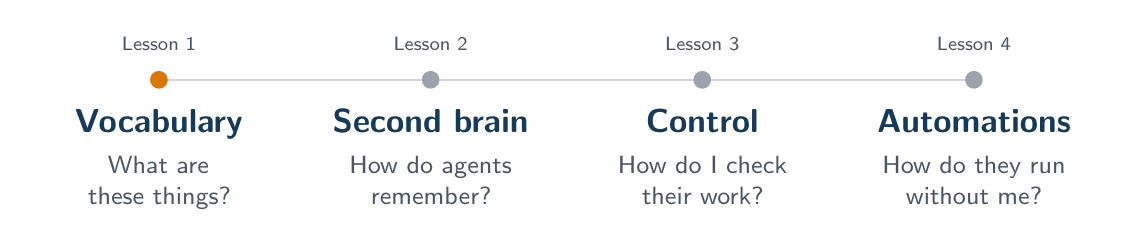
\begin{tikzpicture}[x=3.45cm]
    \draw[hair,line width=0.6pt] (0,0) -- (3,0);
    \foreach \x/\name/\q/\c in {%
      0/Vocabulary/What are these things?/accent,%
      1/Second brain/How do agents remember?/faint,%
      2/Control/How do I check their work?/faint,%
      3/Automations/How do they run without me?/faint}{%
      \fill[\c] (\x,0) circle (3.2pt);
      \node[anchor=south,font=\scriptsize,text=muted] at (\x,0.25) {Lesson \the\numexpr\x+1\relax};
      \node[anchor=north,font=\large\bfseries,text=ink] at (\x,-0.25) {\name};
      \node[anchor=north,font=\small,text=muted,text width=3.1cm,align=center] at (\x,-0.85) {\q};
    }
  \end{tikzpicture}
  \end{center}
  \vfill
  {\color{muted}\small Today is the map. The next three lessons build on these words.\par}
\end{frame}

% -------- Twelve words for today --------
\begin{frame}{Twelve words for today}
  \vspace{0.8em}
  \begin{columns}[T,onlytextwidth]
    \column{0.31\textwidth}
      \group{What an agent is}
      {\large model\\[0.25em] harness\\[0.25em] agent\\[0.25em] tool and permission\par}
    \column{0.31\textwidth}
      \group{What it sees}
      {\large prompt\\[0.25em] context window\\[0.25em] token\\[0.25em] compaction\par}
    \column{0.31\textwidth}
      \group{How you extend it}
      {\large rules file\\[0.25em] MCP\\[0.25em] skill\\[0.25em] sub-agent\par}
  \end{columns}
  \vfill
  {\color{muted}\small By the end you should be able to define each one in a sentence. The last slide checks.\par}
\end{frame}

% =============================================================
% From chat to agent
% =============================================================

\sectionframe[What changes when the model can act]{From chat to agent}

% -------- Model + harness = agent --------
\begin{frame}{Model plus harness equals agent}
  \begin{columns}[c,onlytextwidth]
    \column{0.47\textwidth}
      \defn{Harness}{The runtime layer that wraps a language model and turns it into an agent that can act: it runs the loop, exposes tools, manages context and enforces controls.}{\citet{macedo_2026_harness}; \citet{barbaste_2026_harness}}
      \vspace{0.9em}
      {\small\color{muted}Not a harness: an agent framework such as LangChain, or an evaluation harness such as SWE-bench's. Across eleven production harnesses, none imports a general agent framework.\par}
    \column{0.49\textwidth}
      \begin{center}
      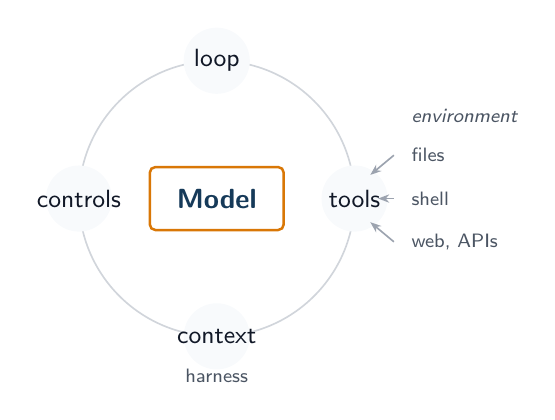
\begin{tikzpicture}
        \draw[hair,line width=0.6pt] (0,0) circle (1.75cm);
        \node[accb,minimum width=1.7cm,minimum height=0.8cm,font=\bfseries,text=ink] (m) at (0,0) {Model};
        \foreach \a/\t in {90/loop,0/tools,270/context,180/controls}{
          \fill[paper] (\a:1.75) circle (0.42cm);
          \node[lab] at (\a:1.75) {\t};
        }
        \node[sub,anchor=west] at (2.35,0.55) {files};
        \node[sub,anchor=west] at (2.35,0) {shell};
        \node[sub,anchor=west] at (2.35,-0.55) {web, APIs};
        \draw[arr] (2.25,0.55) -- (1.95,0.3);
        \draw[arr] (2.25,0) -- (2.05,0);
        \draw[arr] (2.25,-0.55) -- (1.95,-0.3);
        \node[sub] at (0,-2.25) {harness};
        \node[sub,anchor=west] at (2.35,1.05) {\itshape environment};
      \end{tikzpicture}
      \end{center}
  \end{columns}
  \takeaway{Same model, different harness: a different agent.}
\end{frame}

% -------- Chatbot vs agent --------
\begin{frame}{Chatbot vs agent}
  \vspace{0.6em}
  \begin{center}
  \renewcommand{\arraystretch}{1.25}
  \begin{tabularx}{0.86\linewidth}{>{\bfseries\color{ink}}l X X}
  \toprule
   & \leavevmode\color{muted}Chatbot & \leavevmode\color{muted}Agent\\
  \midrule
  Who runs the loop & You & The harness\\
  Unit of delegation & An answer & A task\\
  Files & Pasted or attached & Read, edited, created\\
  Failure mode & A wrong \emph{answer} & A wrong \emph{action}\\
  Your role & Reader & Supervisor\\
  \bottomrule
  \end{tabularx}
  \end{center}
  \takeaway{Different failure mode, different control.}
\end{frame}

% -------- The loop, in a real trace --------
\begin{frame}{The loop, in a real trace}
  \begin{columns}[T,onlytextwidth]
    \column{0.36\textwidth}
      \vspace{0.3em}
      {\small
      \group{Observe}{\color{muted}reads the do-file\par}
      \vspace{0.45em}
      \group{Act}{\color{muted}runs Stata in batch\par}
      \vspace{0.45em}
      \group{Observe}{\color{muted}exit code 0, yet the log says \texttt{prise not found}\par}
      \vspace{0.45em}
      \group{Act}{\color{muted}edits one line\par}
      \vspace{0.45em}
      \group{Verify}{\color{muted}reruns, shows the end of the log, as \texttt{AGENTS.md} asks\par}}
    \column{0.60\textwidth}
      \filebox{assets/lesson1/traces/loop_excerpt.txt}{Real run on the course demo repository, 26 Oct 2026: OpenCode with DeepSeek V4.1 Flash (free tier), 22 seconds. Paths shortened.}
  \end{columns}
\end{frame}

% -------- Timeline --------
\begin{frame}{From chat window to command center}
  \vspace{1.2em}
  \begin{center}
  
\begin{tikzpicture}[x=2.72cm]
    \draw[hair,line width=0.6pt] (-0.1,0) -- (4.1,0);
    \foreach \x/\d/\e/\c in {%
      0/Nov 2022/ChatGPT: a chat window/faint,%
      1/Feb 2025/Claude Code: an agent in the terminal/faint,%
      2/Feb 2026/Codex app: ``a command center for agents''/faint,%
      3/Jul 2026/Codex merges into the ChatGPT desktop app/accent,%
      4/Sep 2026/Claude: Chat and Cowork become one/accent}{%
      \fill[\c] (\x,0) circle (2.8pt);
      \node[anchor=south,font=\scriptsize\bfseries,text=ink] at (\x,0.22) {\d};
      \node[anchor=north,font=\small,text=dark,text width=2.45cm,align=center] at (\x,-0.25) {\e};
    }
  \end{tikzpicture}
  \end{center}
  \vfill
  \takeaway{The interface no longer tells you whether you are chatting or delegating.}
  \source{\citet{openai_2026_chatgptapp}; \citet{anthropic_2026_oneclaude}; OpenAI, \emph{Introducing the Codex app}, 2 Feb 2026.}
\end{frame}

% -------- METR --------
\begin{frame}{How long a task can an agent finish?}
  \begin{columns}[T,onlytextwidth]
    \column{0.64\textwidth}
      \shot{metr_time_horizon.png}{METR, Time Horizon 1.1. Captured 26 Oct 2026.}
    \column{0.32\textwidth}
      \vspace{0.2em}
      {\small
      \group{What it measures}
      {\color{muted}The length of software tasks, timed on human experts, that a model completes half of the time.\par}
      \vspace{0.7em}
      \group{What it does not}
      {\color{muted}How long an agent works alone. Economics tasks. Anything above 16 hours, which METR calls unreliable.\par}
      \vspace{0.7em}
      \group{Status}
      {\color{muted}Page frozen on 8 Sep 2026.\par}}
  \end{columns}
\end{frame}

% -------- Demo 1 --------
\demoframe{Live: chat vs agent}{%
  {\small
  The do-file in the demo repository fails.\\[0.4em]
  First, paste it into a chat window and ask for the bug.\\[0.4em]
  Then give the same sentence to an agent opened in the repository folder.\par}}{%
  {\small
  Who runs Stata.\\[0.4em]
  Who reads the log.\\[0.4em]
  What you have to check at the end.\par}}

\begin{frame}{Recorded result: what the agent left behind}
  \begin{columns}[T,onlytextwidth]
    \column{0.42\textwidth}
      \group{The change}
      \begin{tcolorbox}[l1base,colback=white,borderline={0.4pt}{0pt}{hair},left=0.6em,top=0.4em,bottom=0.4em]
        \ttfamily\footnotesize
        {\color{bad}- gen lprice = ln(prise)}\\
        {\color{good}+ gen lprice = ln(price)}
      \end{tcolorbox}
      \vspace{0.9em}
      {\small\color{muted}One line in the do-file. The data are untouched, as the rules file asks.\par}
      \vspace{0.9em}
      {\small\color{muted}The table runs, but look at the empty base-category rows: ``done'' still needs a reader. Lesson 3.\par}
    \column{0.54\textwidth}
      \group{The output}
      \begin{tcolorbox}[l1base,colback=white,borderline={0.4pt}{0pt}{hair},halign=center,top=0.3em,bottom=0.3em]
        \resizebox*{!}{5.3cm}{{
\def\sym#1{\ifmmode^{#1}\else\(^{#1}\)\fi}
\begin{tabular}{l*{2}{c}}
\toprule
                    &\multicolumn{1}{c}{(1)}&\multicolumn{1}{c}{(2)}\\
                    &\multicolumn{1}{c}{lprice}&\multicolumn{1}{c}{lprice}\\
\midrule
l100km              &      0.0217         &      0.0193         \\
                    &    (0.0309)         &    (0.0331)         \\
\addlinespace
Weight (lbs.)       &    0.000377\sym{*}  &    0.000406\sym{*}  \\
                    &  (0.000145)         &  (0.000153)         \\
\addlinespace
Domestic            &           0         &           0         \\
                    &         (.)         &         (.)         \\
\addlinespace
Foreign             &       0.503\sym{***}&       0.486\sym{***}\\
                    &     (0.102)         &     (0.140)         \\
\addlinespace
Repair record 1978=1&                     &           0         \\
                    &                     &         (.)         \\
\addlinespace
Repair record 1978=2&                     &      0.0372         \\
                    &                     &     (0.132)         \\
\addlinespace
Repair record 1978=3&                     &      0.0793         \\
                    &                     &    (0.0923)         \\
\addlinespace
Repair record 1978=4&                     &       0.102         \\
                    &                     &     (0.114)         \\
\addlinespace
Repair record 1978=5&                     &       0.146         \\
                    &                     &     (0.141)         \\
\addlinespace
Constant            &       7.095\sym{***}&       6.942\sym{***}\\
                    &     (0.199)         &     (0.215)         \\
\midrule
Observations        &          74         &          69         \\
\bottomrule
\multicolumn{3}{l}{\footnotesize Standard errors in parentheses}\\
\multicolumn{3}{l}{\footnotesize \sym{*} \(p<0.05\), \sym{**} \(p<0.01\), \sym{***} \(p<0.001\)}\\
\end{tabular}
}
}
      \end{tcolorbox}
      {\color{muted}\scriptsize \texttt{output/table1.tex} as written by the agent, compiled unedited.\par}
  \end{columns}
\end{frame}

% =============================================================
% Core vocabulary
% =============================================================

\sectionframe[What the agent sees, and how you extend it]{Core vocabulary}

% -------- Prompt vs task --------
\begin{frame}{Prompt vs task}
  \begin{columns}[T,onlytextwidth]
    \column{0.44\textwidth}
      \defn{Prompt}{``Explain how to cluster standard errors in Stata.''}{One question, one answer. No state, no side effects.}
      \vspace{0.8em}
      \defn{Task}{``Rerun both models with clustered errors, regenerate the table, tell me what changed.''}{A goal, a workflow, an artefact you can check.}
    \column{0.50\textwidth}
      \group{A task an agent can finish names four things}
      \vspace{0.3em}
      \renewcommand{\arraystretch}{1.35}
      \begin{tabularx}{\linewidth}{>{\bfseries\color{ink}}l X}
        Goal & what should exist at the end\\
        Inputs & which files, which data\\
        Limits & what must not change\\
        Done & how you will check it\\
      \end{tabularx}
  \end{columns}
  \takeaway{Agents change the unit of delegation.}
\end{frame}

% -------- Context window and tokens --------
\pgfplotstableread[col sep=comma]{assets/lesson1/charts/data/context_windows.csv}\ctxtable
\begin{frame}{Context window and tokens}
  \begin{columns}[c,onlytextwidth]
    \column{0.58\textwidth}
      \begin{tikzpicture}
        \begin{axis}[l1axis,
            width=0.82\linewidth,height=5.4cm,
            xbar,bar width=7pt,bar shift=0pt,
            xmode=log,log basis x=10,log origin x=infty,
            xmin=5000,xmax=2000000,
            xtick={10000,100000,1000000},
            xticklabels={10k,100k,1M},
            ytick={0,...,7},y dir=reverse,
            ymin=-0.6,ymax=7.6,
            unbounded coords=discard,
            yticklabels from table={\ctxtable}{label},
            yticklabel style={font=\scriptsize,color=dark},
            xlabel={tokens the model can see at once (log scale)},
            nodes near coords,
            point meta=explicit symbolic,
            nodes near coords style={font=\scriptsize,color=muted,anchor=west},
          ]
          \addplot[draw=none,fill=faint,only if={group}{past}]
            table[x=tokens,y expr=\coordindex,meta=show]{\ctxtable};
          \addplot[draw=none,fill=ink,only if={group}{now}]
            table[x=tokens,y expr=\coordindex,meta=show]{\ctxtable};
        \end{axis}
      \end{tikzpicture}
    \column{0.38\textwidth}
      {\small
      \group{Token}
      {\color{muted}The unit models read, write and bill. A 30-page paper is roughly 25k.\par}
      \vspace{0.6em}
      \group{Context window}
      {\color{muted}Everything the model sees in one turn: rules, files, tool output, history.\par}
      \vspace{0.6em}
      \group{Context rot}
      {\color{muted}Accuracy falls as the window fills. A bigger window is not a better memory.\par}}
  \end{columns}
  \source{vendor model pages and Artificial Analysis, read 26 Oct 2026; \texttt{context\_windows.csv}.}
\end{frame}

% -------- Compaction --------
\begin{frame}{Compaction}
  \defn{Compaction}{Taking a conversation nearing the context window limit, summarizing its contents, and reinitiating a new context window with the summary.}{\citet{anthropic_2025_context}. In Codex and Claude Code: \texttt{/compact}. Most harnesses also do it on their own.}
  \vspace{0.9em}
  \begin{center}
  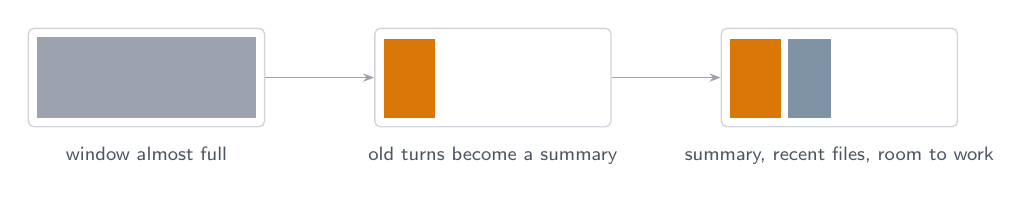
\begin{tikzpicture}
    \tikzset{win/.style={draw=hair,line width=0.5pt,rounded corners=2pt,fill=white,minimum width=3.0cm,minimum height=1.25cm}}
    \node[win] (a) at (0,0) {};
    \fill[faint] ($(a.south west)+(0.12,0.12)$) rectangle ($(a.north east)+(-0.12,-0.12)$);
    \node[sub,below=0.12cm of a] {window almost full};
    \node[win] (b) at (4.4,0) {};
    \fill[accent] ($(b.south west)+(0.12,0.12)$) rectangle ++(0.65,1.01);
    \node[sub,below=0.12cm of b] {old turns become a summary};
    \node[win] (c) at (8.8,0) {};
    \fill[accent] ($(c.south west)+(0.12,0.12)$) rectangle ++(0.65,1.01);
    \fill[ink!55] ($(c.south west)+(0.85,0.12)$) rectangle ++(0.55,1.01);
    \node[sub,below=0.12cm of c] {summary, recent files, room to work};
    \draw[arr] (a.east) -- (b.west);
    \draw[arr] (b.east) -- (c.west);
  \end{tikzpicture}
  \end{center}
  \takeaway{A summary loses detail. Decisions belong in files.}
\end{frame}

% -------- Rules files --------
\begin{frame}{Rules files: prompts that stay}
  \begin{columns}[T,onlytextwidth]
    \column{0.56\textwidth}
      \filebox{assets/lesson1/files/AGENTS_excerpt.md}{\texttt{AGENTS.md} of the course demo repository (excerpt). The agent reads it at every session start.}
    \column{0.40\textwidth}
      \vspace{0.2em}
      {\small
      \group{Where the agent is}
      {\color{muted}Layout of the project, what is raw and what is output.\par}
      \vspace{0.6em}
      \group{What it must not do}
      {\color{muted}Never touch the data. No new packages without asking.\par}
      \vspace{0.6em}
      \group{What ``done'' means}
      {\color{muted}Run the do-file and show the end of the log.\par}
      \vspace{0.9em}
      {\color{muted}Same idea, different names: \texttt{AGENTS.md}, \texttt{CLAUDE.md}, \texttt{.cursor/rules}.\par}}
  \end{columns}
\end{frame}

% -------- Tools, permissions, sandbox --------
\begin{frame}{Tools, permissions, sandbox}
  \begin{columns}[c,onlytextwidth]
    \column{0.52\textwidth}
      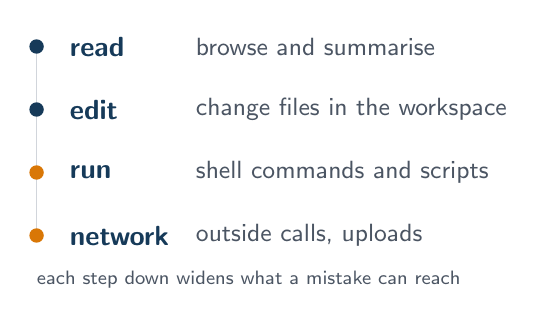
\begin{tikzpicture}[y=-0.8cm]
        \draw[hair,line width=0.6pt] (0,0) -- (0,3);
        \foreach \i/\t/\s/\c in {0/read/browse and summarise/ink,1/edit/change files in the workspace/ink,2/run/shell commands and scripts/accent,3/network/{outside calls, uploads}/accent}{
          \fill[\c] (0,\i) circle (2.6pt);
          \node[anchor=west,font=\bfseries,text=ink] at (0.3,\i) {\t};
          \node[anchor=west,font=\small,text=muted] at (1.9,\i) {\s};
        }
        \node[anchor=west,font=\scriptsize,text=muted] at (-0.12,3.7) {each step down widens what a mistake can reach};
      \end{tikzpicture}
      \par\vspace{0.8em}
      {\small
      \textbf{\color{ink}Tool}: a function the harness lets the model call.\\[0.25em]
      \textbf{\color{ink}Permission}: the line between proposing and doing.\\[0.25em]
      \textbf{\color{ink}Sandbox}: a place where doing is reversible.\par}
    \column{0.42\textwidth}
      \shot{codex_permission_prompt_crop.png}{Codex asks before running a command. OpenAI, \emph{Unlocking the Codex harness}, 2026.}
  \end{columns}
\end{frame}

% -------- MCP --------
\begin{frame}{MCP: one plug for many tools}
  \defn{Model Context Protocol}{An open standard for connecting AI applications to external systems. The harness is the client; each server exposes tools, data and prompts.}{\citet{mcp_spec}}
  \vspace{0.2em}
  \begin{center}
    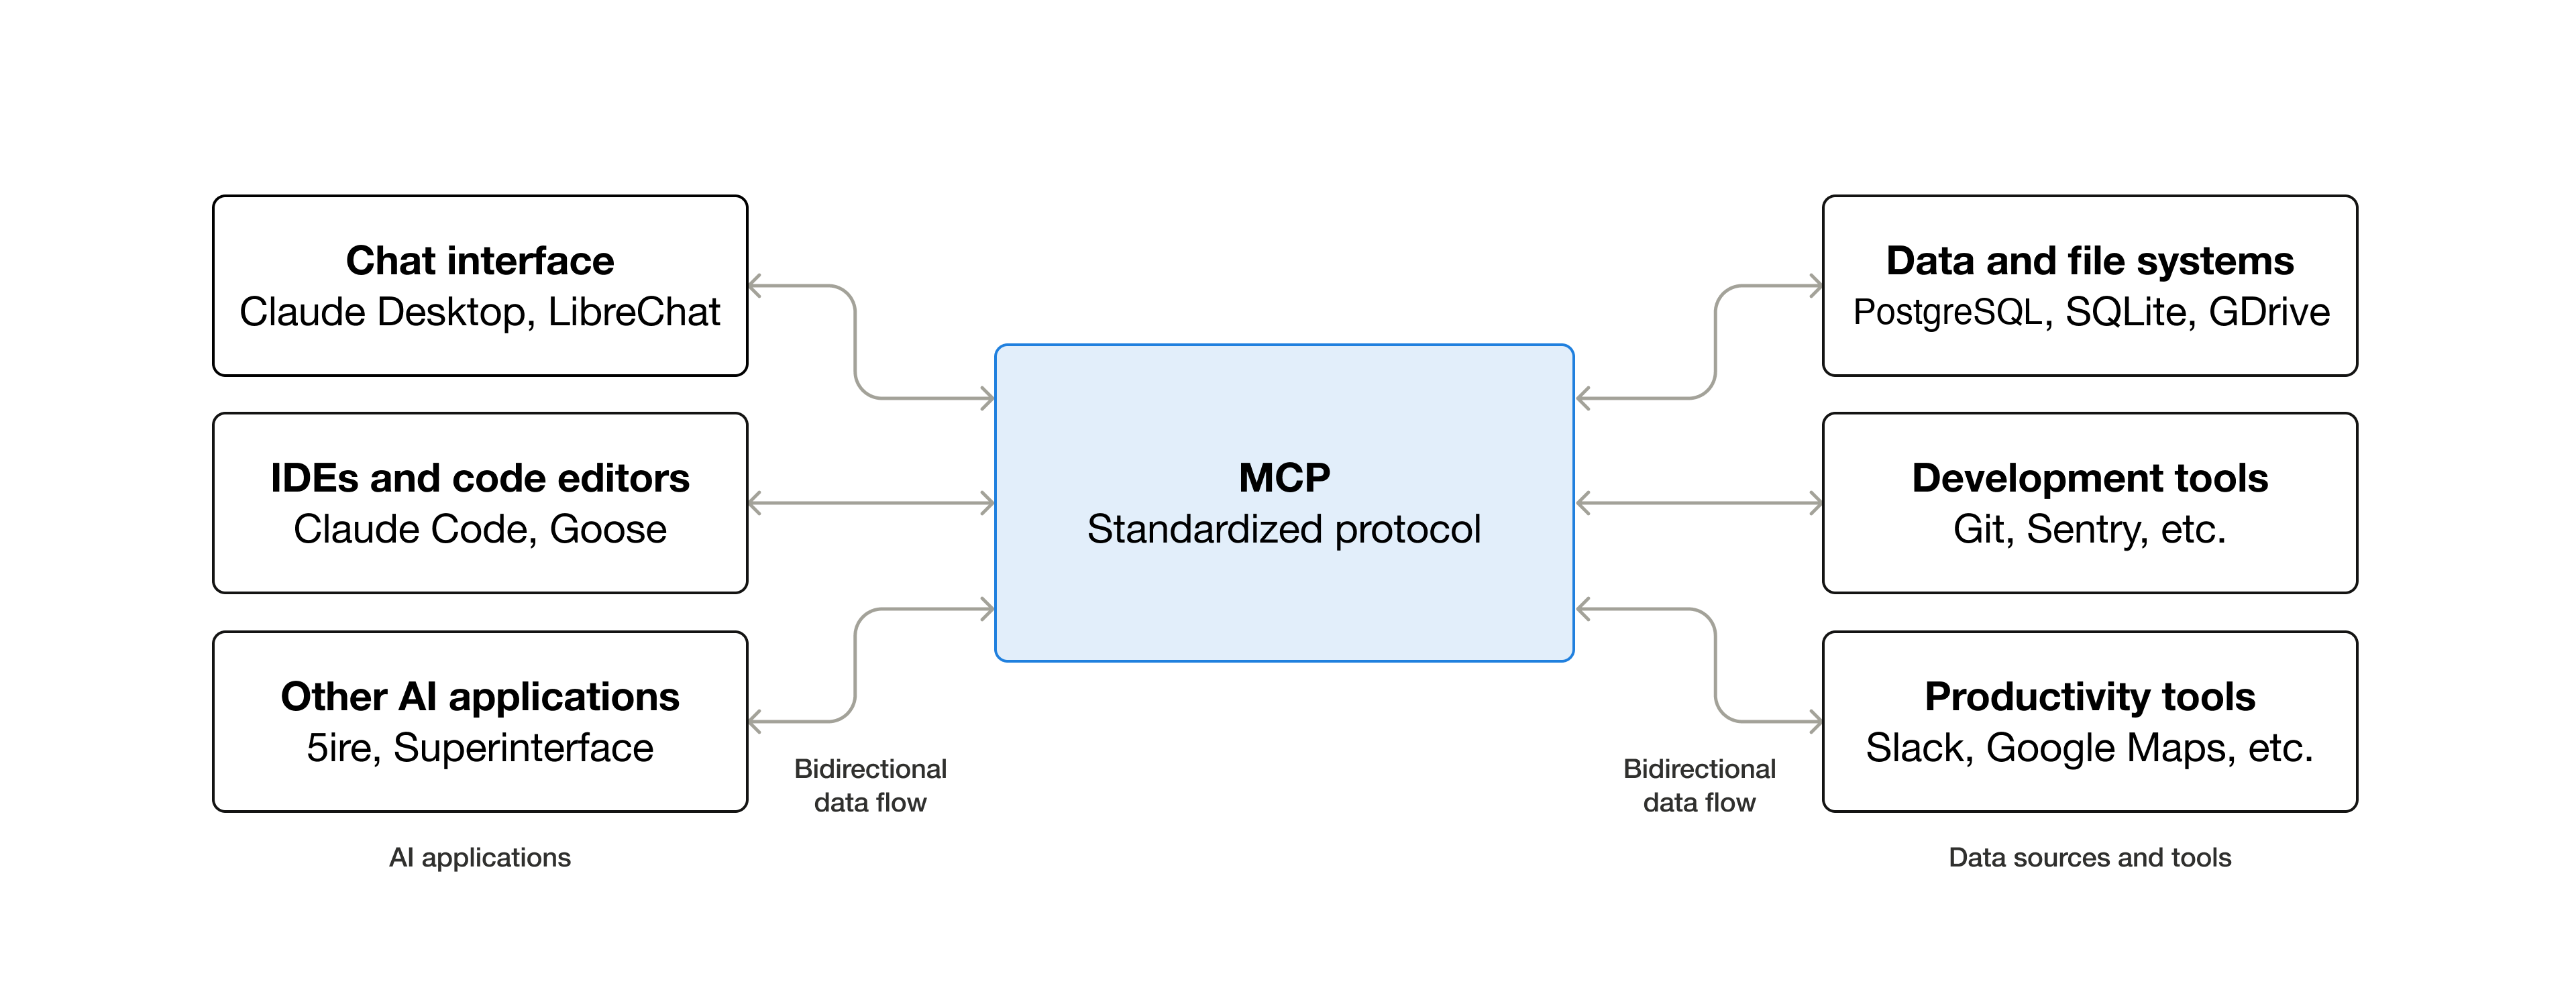
\includegraphics[width=0.54\linewidth]{mcp_simple_diagram.png}
  \end{center}
  \vspace{-0.4em}
  {\small\color{muted}Cost to remember: every connected server adds its tool descriptions to the context before the task starts.\par}
  \source{diagram from modelcontextprotocol.io, read 26 Oct 2026.}
\end{frame}

% -------- Skills --------
\begin{frame}{Skills: procedures the agent loads on demand}
  \begin{columns}[T,onlytextwidth]
    \column{0.52\textwidth}
      \filebox{assets/lesson1/files/SKILL.md}{A real skill from the demo repository.}
    \column{0.44\textwidth}
      {\small
      \defn{Skill}{A folder with a \texttt{SKILL.md} file: a name, a description, instructions, and optional scripts and references.}{\citet{agentskills_spec}}
      \vspace{0.7em}
      \group{Loaded in three steps}
      {\color{muted}Discovery: name and description only.\\
      Activation: the full file, when a request matches.\\
      Execution: scripts and references, if needed.\par}
      \vspace{0.7em}
      {\color{muted}Nine of eleven production harnesses read \texttt{SKILL.md}; eight speak MCP \citep{barbaste_2026_harness}.\par}}
  \end{columns}
\end{frame}

% -------- Sub-agents and hooks --------
\begin{frame}{Sub-agents and hooks}
  \vspace{0.6em}
  \begin{columns}[T,onlytextwidth]
    \column{0.47\textwidth}
      \group{Sub-agent}
      {\small An agent started by the main agent, with its own context and one narrow job. It hands back a short report and keeps its history.\par}
      \vspace{0.6em}
      {\small\color{muted}
      A reviewer that reads the diff before a commit.\\[0.2em]
      An explorer that searches a large repository.\\[0.2em]
      A Stata runner that returns only the table.\par}
    \column{0.47\textwidth}
      \group{Hook}
      {\small A fixed command the harness runs at a set moment, whatever the model thinks. It is code; the model cannot skip it.\par}
      \vspace{0.6em}
      {\small\color{muted}
      At session start: load the rules and the project state.\\[0.2em]
      After an edit: run a linter or a prose check.\\[0.2em]
      Before a commit: block secrets and raw data.\par}
  \end{columns}
  \takeaway{Sub-agents delegate judgement. Hooks remove it. Lesson 4 builds both.}
\end{frame}

% -------- Memory has layers --------
\begin{frame}{Memory has layers}
  \vspace{1.0em}
  \begin{center}
  
\begin{tikzpicture}[x=3.4cm]
    \foreach \x/\n/\q/\s in {%
      0/Session/What did we just say?/frameb,%
      1/Project/What is this project?/accb,%
      2/Persistent/What did I decide before?/frameb,%
      3/Graph/How is it all connected?/frameb}{%
      \node[\s,minimum width=2.8cm,minimum height=0.95cm,font=\bfseries,text=ink] (n\x) at (\x,0) {\n};
      \node[sub,text width=2.8cm,anchor=north] at (\x,-0.7) {\q};
    }
    \foreach \x [evaluate=\x as \y using int(\x+1)] in {0,1,2}{\draw[arr] (n\x.east) -- (n\y.west);}
  \end{tikzpicture}
  \end{center}
  \vspace{0.8em}
  {\small\color{muted}\centering The context window is only the first layer. Compaction is why the others exist.\par}
  \takeaway{Lesson 2 builds the project layer: the one researchers use least.}
\end{frame}

% -------- Demo 2 and 3 --------
\demoframe{Live: context, MCP and skills}{%
  {\small
  Watch the context meter while the agent works, then run \texttt{/compact} and read the summary it keeps.\\[0.4em]
  List the MCP servers the harness can reach.\\[0.4em]
  Ask for ``a regression table'' and see which skill it loads.\par}}{%
  {\small
  What the summary drops.\\[0.4em]
  Which tools appear without being asked for.\\[0.4em]
  When \texttt{SKILL.md} gets read.\par}}

\begin{frame}{Recorded result: the skill was read when the request matched}
  \begin{columns}[T,onlytextwidth]
    \column{0.64\textwidth}
      \filebox{assets/lesson1/traces/skill_excerpt.txt}{Real run, 26 Oct 2026: OpenCode with DeepSeek V4.1 Flash (free tier), 57 seconds. Paths shortened.}
    \column{0.32\textwidth}
      \vspace{0.2em}
      {\small
      {\color{muted}The request said ``regression table''. The skill's description said the same. The agent opened \texttt{SKILL.md} second, before touching Stata.\par}
      \vspace{0.8em}
      {\color{muted}Stars, statistics and the closing report come from the skill. The prompt never asked for them.\par}}
  \end{columns}
\end{frame}

% =============================================================
% Harnesses in 2026
% =============================================================

\sectionframe[Where you meet agents, and why the window matters less]{Harnesses in 2026}

% -------- Five surfaces --------
\begin{frame}{Five surfaces, one idea}
  \begin{center}
  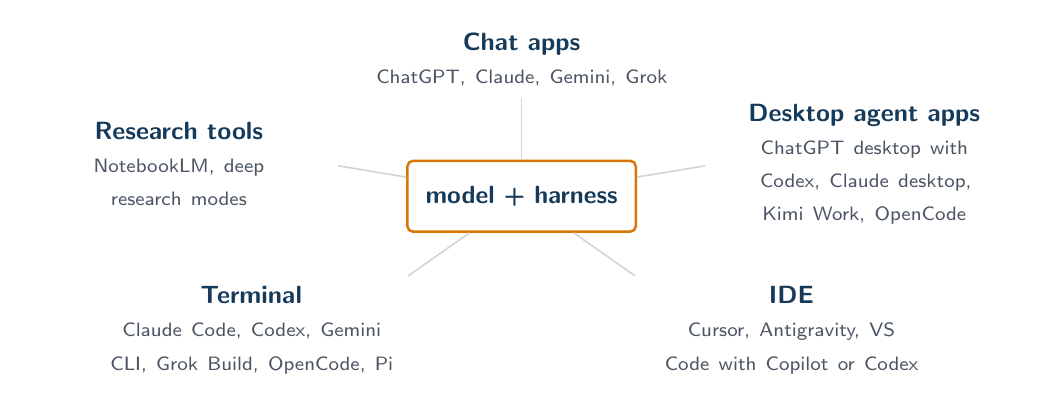
\begin{tikzpicture}
    \node[accb,minimum width=2.9cm,minimum height=0.9cm,align=center,font=\small\bfseries,text=ink] (h) at (0,0) {model + harness};
    \foreach \a/\n/\p/\an in {%
      90/Chat apps/{ChatGPT, Claude, Gemini, Grok}/south,%
      18/Desktop agent apps/{ChatGPT desktop with Codex, Claude desktop, Kimi Work, \rev{OpenCode}}/west,%
      -54/IDE/{Cursor, Antigravity, VS Code with Copilot or Codex}/north west,%
      -126/Terminal/{Claude Code, \rev{Codex}, Gemini CLI, Grok Build, OpenCode, Pi}/north east,%
      162/Research tools/{NotebookLM, deep research modes}/east}{%
      \draw[hair,line width=0.6pt] (h) -- ({2.45*cos(\a)},{1.25*sin(\a)});
      \node[anchor=\an,align=center,text width=3.7cm,inner sep=2pt] at ({2.55*cos(\a)},{1.32*sin(\a)})
        {{\small\bfseries\color{ink}\n}\\{\scriptsize\color{muted}\p}};
    }
  \end{tikzpicture}
  \end{center}
  \vfill
  \takeaway{Pick the surface for the task. The loop underneath is the same.}
\end{frame}

% -------- Chat became agent --------
\begin{frame}{Chat became agent}
  \begin{columns}[c,onlytextwidth]
    \column{0.52\textwidth}
      \shot{chatgpt_app_proactive_teammate_v2.png}{ChatGPT desktop: Chat, Work and Codex in one window since 9 Jul 2026.}
    \column{0.44\textwidth}
      {\small\rev{Claude is on the same path. From 16 Sep 2026, Chat and Cowork are merging into one conversation. The rollout is still incomplete.}\par}
      \vspace{0.8em}
      {\small\rev{You can still tell Chat from Work, and you can still switch. What is changing is the merger into one harness.}\par}
  \end{columns}
\end{frame}

\begin{frame}{The terminal, on its own}
  \begin{columns}[c,onlytextwidth]
    \column{0.46\textwidth}
      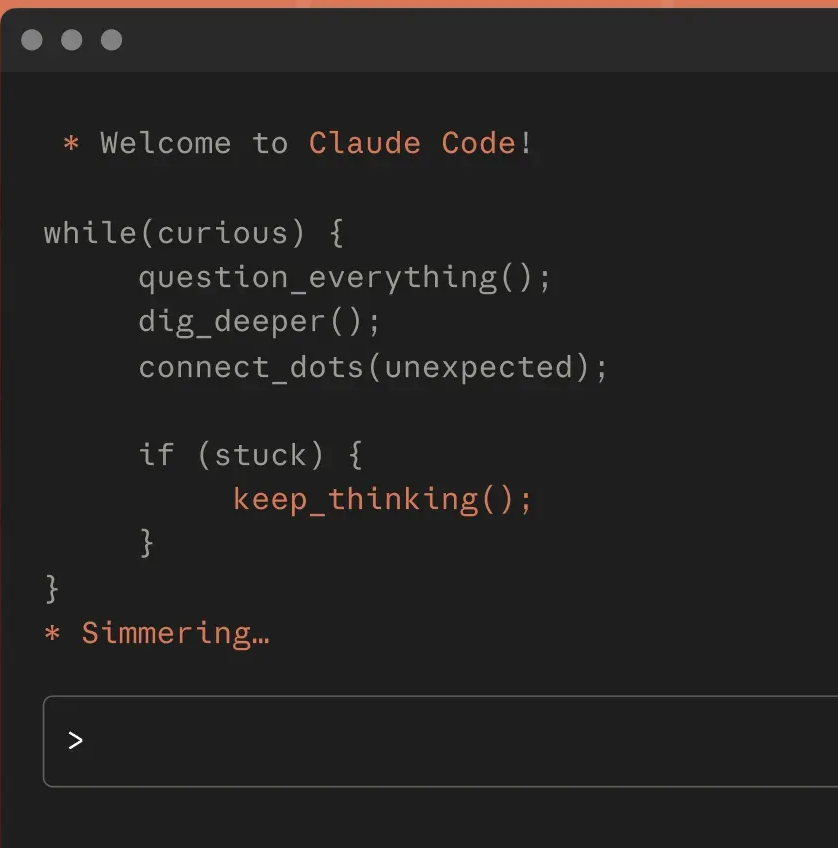
\includegraphics[height=5.2cm]{claude_code_terminal.png}
      \par\vspace{0.12em}{\scriptsize\rev{Claude Code in the shell.}\par}
    \column{0.50\textwidth}
      {\small
      \group{What it is}
      {\rev{You type in a shell. The agent reads the folder, runs commands and edits files. Claude Code and Codex both work this way.}\par}
      \vspace{0.7em}
      \group{Where it pays}
      {\rev{Scriptable. Runs on a server. Every step is text you can log.}\par}
      \vspace{0.7em}
      \group{Open harnesses}
      {\rev{OpenCode, Pi, Aider, OpenHands. OpenCode also has an app. You bring the model, through an API key or OpenRouter.}\par}}
  \end{columns}
\end{frame}

% -------- IDE agents --------
\begin{frame}{IDE agents: review is a diff}
  \begin{columns}[T,onlytextwidth]
    \column{0.55\textwidth}
      \shot{antigravity_ide.png}{Google Antigravity.}
    \column{0.41\textwidth}
      \shoth{codex_vscode.png}{3.5cm}{Codex inside VS Code.}
      \par\vspace{0.7em}
      {\small\color{muted}Every change arrives as a diff you accept or reject, line by line.\par}
  \end{columns}
\end{frame}

% -------- Choose by task --------
\begin{frame}{Start from the task}
  \vspace{0.6em}
  \begin{center}
  \renewcommand{\arraystretch}{1.3}
  \begin{tabularx}{0.88\linewidth}{>{\leavevmode\color{dark}}X >{\bfseries\color{ink}}l}
  \toprule
  \color{muted}If the job is & \color{muted}start with\\
  \midrule
  Thinking, writing, reading a paper & a chat app\\
  Sources and evidence across many documents & a research tool\\
  Work on a project folder, with files you review & a desktop agent app or an IDE\\
  Batch jobs, servers, anything you want logged & a terminal harness\\
  Data that must not leave the machine & a local model in an open harness\\
  \bottomrule
  \end{tabularx}
  \end{center}
  \takeaway{Most real work combines two of these.}
\end{frame}

% =============================================================
% Models and benchmarks
% =============================================================

\sectionframe[Who builds them, how to compare them, what people use]{Models and benchmarks}

% -------- Who builds frontier models --------
\begin{frame}{Who builds frontier models, October 2026}
  \vspace{0.4em}
  \begin{columns}[T,onlytextwidth]
    \column{0.48\textwidth}
      \group{United States, closed weights}
      \renewcommand{\arraystretch}{1.3}
      \begin{tabularx}{\linewidth}{>{\bfseries\color{ink}}l >{\small\leavevmode\color{dark}}X}
        Anthropic & Claude Opus 5.5, Sonnet 5.5, Fable 5.1, Haiku 5.5\\
        OpenAI & GPT-6 Astra, GPT-6.1 Sol, GPT-6 Luna\\
        Google & Gemini 4 Argon\\
        Meta & Muse Wonder, Muse Wonder Full\\
        SpaceXAI & Grok 4.7\\
      \end{tabularx}
    \column{0.48\textwidth}
      \group{China, mostly open weights}
      \renewcommand{\arraystretch}{1.3}
      \begin{tabularx}{\linewidth}{>{\bfseries\color{ink}}l >{\small\leavevmode\color{dark}}X}
        DeepSeek & DeepSeek V4.1 Flash\\
        Z.ai & GLM-5.3, GLM-5.3 Flash\\
        Moonshot & Kimi K3, Kimi K3.1 Pro\\
        Alibaba & Qwen3.8\\
        Xiaomi & MiMo-V2.6 Pro and Flash\\
      \end{tabularx}
  \end{columns}
  \vfill
  {\small\color{muted}Frontier releases now arrive weeks apart: Grok 4.7 on 21 Sep, Opus 5.5 on 22 Sep, Muse Wonder on 12 Oct, Kimi K3.1 Pro on 23 Oct.\par}
  \source{vendor release pages; Artificial Analysis model list, read 26 Oct 2026.}
\end{frame}

% -------- One independent index --------
\pgfplotstableread[col sep=comma]{assets/lesson1/charts/data/aa_index_2026-10.csv}\aatable
\begin{frame}{One independent index}
  \begin{columns}[c,onlytextwidth]
    \column{0.60\textwidth}
      \begin{tikzpicture}
        \begin{axis}[l1axis,
            width=0.8\linewidth,height=6.1cm,
            xbar,bar width=6pt,bar shift=0pt,
            xmin=0,xmax=64,
            xtick={0,20,40,60},
            ytick={0,...,11},y dir=reverse,
            ymin=-0.6,ymax=11.6,
            yticklabels from table={\aatable}{model},
            yticklabel style={font=\scriptsize,color=dark},
            xlabel={Artificial Analysis Intelligence Index},
            nodes near coords,
            nodes near coords style={font=\scriptsize,color=muted,anchor=west},
            unbounded coords=discard,
          ]
          \addplot[draw=none,fill=ink,only if={weights}{closed}]
            table[x=index,y expr=\coordindex]{\aatable};
          \addplot[draw=none,fill=accent,only if={weights}{open}]
            table[x=index,y expr=\coordindex]{\aatable};
        \end{axis}
      \end{tikzpicture}
    \column{0.36\textwidth}
      {\small
      {\color{accent}\bfseries Orange}: weights you can download today. {\color{ink}\bfseries Blue}: API only.\par
      \vspace{0.7em}
      {\color{muted}The best open-weight model sits 12 points below the top.\par}
      \vspace{0.7em}
      {\color{muted}Kimi K3.1 Pro is called open-weight at launch; the weights are promised for 4 Nov. Until then, it is a closed model.\par}
      \vspace{0.7em}
      {\color{muted}gpt-oss-120b is shown as the strongest US open-weight reference.\par}}
  \end{columns}
  \source{\citet{aa_2026_index}, best setting per model, read 26 Oct 2026; \texttt{aa\_index\_2026-10.csv}.}
\end{frame}

% -------- How to read a benchmark --------
\begin{frame}{How to read a benchmark}
  \begin{columns}[c,onlytextwidth]
    \column{0.45\textwidth}
      {\small
      \group{Who ran it}
      {\color{muted}An independent lab, or the vendor's own launch post? Launch charts often reuse rivals' self-reported numbers.\par}
      \vspace{0.6em}
      \group{At which setting}
      {\color{muted}Claude Opus 5.5 scores 58 at maximum effort and 42 at low effort. Same model, same week.\par}
      \vspace{0.6em}
      \group{Ranked by what}
      {\color{muted}Capability and use rank models differently. On the right, the same five models on two scales.\par}}
    \column{0.51\textwidth}
      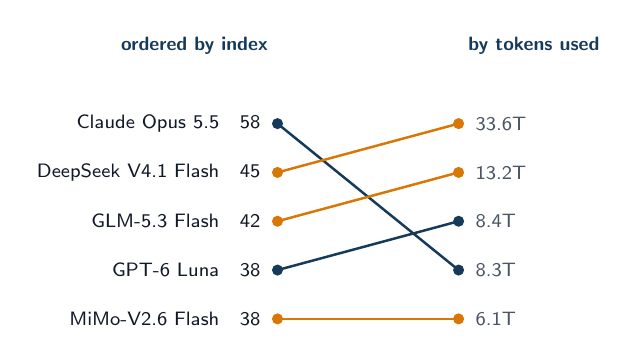
\begin{tikzpicture}[x=2.3cm,y=0.62cm]
        \node[font=\scriptsize\bfseries,text=ink,anchor=east] at (0,6.0) {ordered by index};
        \node[font=\scriptsize\bfseries,text=ink,anchor=west] at (1,6.0) {by tokens used};
        \foreach \l/\a/\s/\b/\t/\c in {%
          Claude Opus 5.5/1/58/4/8.3T/ink,%
          DeepSeek V4.1 Flash/2/45/1/33.6T/accent,%
          GLM-5.3 Flash/3/42/2/13.2T/accent,%
          GPT-6 Luna/4/38/3/8.4T/ink,%
          MiMo-V2.6 Flash/5/38/5/6.1T/accent}{%
          \draw[\c,line width=0.9pt] (0,5.4-\a) -- (1,5.4-\b);
          \fill[\c] (0,5.4-\a) circle (2pt);
          \fill[\c] (1,5.4-\b) circle (2pt);
          \node[anchor=east,font=\scriptsize,text=dark] at (-0.04,5.4-\a) {\l\quad\s};
          \node[anchor=west,font=\scriptsize,text=muted] at (1.04,5.4-\b) {\t};
        }
      \end{tikzpicture}
      \par\vspace{0.2em}{\color{muted}\scriptsize Index: Artificial Analysis. Tokens: OpenRouter, week to 25 Oct 2026.\par}
  \end{columns}
\end{frame}

% -------- Intelligence per dollar --------
\pgfplotstableread[col sep=comma]{assets/lesson1/charts/data/price_vs_index.csv}\pxtable
\begin{frame}{Intelligence per dollar}
  \begin{columns}[c,onlytextwidth]
    \column{0.64\textwidth}
      \begin{tikzpicture}
        \begin{axis}[l1axis,
            width=\linewidth,height=6.0cm,
            xmode=log,xmin=0.04,xmax=12,
            xtick={0.1,1,10},xticklabels={\$0.10,\$1,\$10},
            ymin=34,ymax=61,ytick={40,50,60},
            xlabel={cost to run the index once, per task (log scale)},
            ylabel={index},
            only marks,
            unbounded coords=discard,
          ]
          \addplot[mark=*,mark size=2.2pt,color=ink,only if={weights}{closed}]
            table[x=cost_per_task,y=index]{\pxtable};
          \addplot[mark=*,mark size=2.2pt,color=accent,only if={weights}{open}]
            table[x=cost_per_task,y=index]{\pxtable};
          \foreach \x/\y/\l/\p in {5.98/58/Claude Opus 5.5/east,2.11/55/Kimi K3.1 Pro/east,
              0.72/52/GPT-6.1 Sol/east,0.13/46/MiMo-V2.6-Pro/south west,
              0.26/45/DeepSeek V4.1 Flash/north west,2.01/45/GLM-5.3/north,
              0.21/43/Claude Haiku 5.5/north west,0.07/38/GPT-6 Luna/west}{%
            \edef\temp{\noexpand\node[font=\noexpand\tiny,text=muted,anchor=\p,inner sep=2.5pt] at (axis cs:\x,\y) {\l};}\temp
          }
        \end{axis}
      \end{tikzpicture}
    \column{0.32\textwidth}
      {\small
      {\color{muted}Opus 5.5 costs \$5.98 per task and scores 58.\par}
      \vspace{0.5em}
      {\color{muted}GPT-6.1 Sol costs \$0.72 and scores 52.\par}
      \vspace{0.5em}
      {\color{muted}MiMo-V2.6-Pro, open weights, costs \$0.13 and scores 46.\par}
      \vspace{0.9em}
      {\color{ink}\bfseries About 45 times cheaper for twelve points. Whether that trade is good depends on the task.\par}}
  \end{columns}
  \source{\citet{aa_2026_index}, ``cost per task'' column, read 26 Oct 2026; \texttt{price\_vs\_index.csv}.}
\end{frame}

% -------- What people actually use --------
\pgfplotstableread[col sep=comma]{assets/lesson1/charts/data/openrouter_share_2026-10-19.csv}\ortable
\begin{frame}{What people actually use}
  \begin{columns}[c,onlytextwidth]
    \column{0.56\textwidth}
      \begin{tikzpicture}
        \begin{axis}[l1axis,
            width=\linewidth,height=5.8cm,
            xbar,bar width=6.5pt,bar shift=0pt,
            xmin=0,xmax=31,
            xtick={0,10,20,30},xticklabels={0\%,10\%,20\%,30\%},
            ytick={0,...,9},y dir=reverse,
            ymin=-0.6,ymax=9.6,
            yticklabels from table={\ortable}{author},
            yticklabel style={font=\scriptsize,color=dark},
            xlabel={share of requests on OpenRouter, week of 19 Oct 2026},
            nodes near coords,
            nodes near coords style={font=\scriptsize,color=muted,anchor=west},
            unbounded coords=discard,
          ]
          \addplot[draw=none,fill=accent,only if={country}{CN}]
            table[x=share,y expr=\coordindex]{\ortable};
          \addplot[draw=none,fill=ink,only if={country}{US}]
            table[x=share,y expr=\coordindex]{\ortable};
          \addplot[draw=none,fill=faint,only if={country}{EU}]
            table[x=share,y expr=\coordindex]{\ortable};
          \addplot[draw=none,fill=faint,only if={country}{other}]
            table[x=share,y expr=\coordindex]{\ortable};
        \end{axis}
      \end{tikzpicture}
    \column{0.40\textwidth}
      {\small
      {\color{accent}\bfseries Orange}: Chinese labs. {\color{ink}\bfseries Blue}: US labs.\par
      \vspace{0.7em}
      {\color{muted}Open-weight models have carried more than 62\% of OpenRouter tokens every week since July 2026.\par}
      \vspace{0.7em}
      {\color{ink}\bfseries This is traffic on one router, counted in requests. It is not market share, users or spend.\par}}
  \end{columns}
  \source{\citet{openrouter_2026_rankings} (CC BY 4.0); \citet{openrouter_2026_tokenstate}.}
\end{frame}

% -------- Open weights, open source, local --------
\begin{frame}{Open weights, open source, local}
  \begin{columns}[T,onlytextwidth]
    \column{0.48\textwidth}
      \defn{Open weights}{The trained parameters can be downloaded and run on your own hardware, under the terms of a licence.}{DeepSeek, GLM, Qwen, MiMo, Kimi K3, gpt-oss, Gemma.}
      \vspace{0.7em}
      \defn{Open source AI}{Open weights, plus the training code and enough information about the data to rebuild the model.}{Open Source Initiative, Open Source AI Definition 1.0. Few frontier models qualify.}
    \column{0.46\textwidth}
      {\small
      \group{Licences differ}
      {\color{muted}Kimi K3's licence requires a separate agreement from model-as-a-service businesses above \$20M in yearly revenue. Read the licence before building on a model.\par}
      \vspace{0.6em}
      \group{Local pays off when}
      {\color{muted}data cannot leave the machine, or the same small task runs thousands of times.\par}
      \vspace{0.6em}
      \group{Local hurts when}
      {\color{muted}the task needs frontier reasoning or long agent loops on a laptop. Tools: Ollama, LM Studio.\par}}
  \end{columns}
\end{frame}

% -------- Demo 4 --------
\demoframe{Live: same harness, another model}{%
  {\small
  Run the bug-fixing task from the first demo in OpenCode.\\[0.4em]
  Change one flag, \texttt{-m}, and run it again with a different model.\par}}{%
  {\small
  Time to finish.\\[0.4em]
  Number of steps.\\[0.4em]
  Whether ``done'' is really done.\par}}

\begin{frame}{Recorded result: one task, three models}
  \vspace{0.6em}
  \begin{center}
  \renewcommand{\arraystretch}{1.3}
  \begin{tabular}{>{\bfseries\color{ink}}l l r r l}
\toprule
\color{muted}Model & \color{muted}Weights & \color{muted}Time & \color{muted}Tool calls & \color{muted}Result\\
\midrule
DeepSeek V4.1 Flash (free tier) & open & 22 s & 9 & fixed, table written\\
GLM-5.3 & open & 29 s & 6 & fixed, table written\\
GPT-6 Luna & closed & 42 s & 12 & fixed, table written\\
\bottomrule
\end{tabular}

  \end{center}
  \vfill
  {\small\color{muted}Same harness, same prompt, same repository, same day. Only the \texttt{-m} flag changed. A one-line typo is easy for all three; harder tasks are where models separate.\par}
  \source{runs on 26 Oct 2026; full logs in \texttt{assets/lesson1/traces/}.}
\end{frame}

% =============================================================
% Cost, data, reliability: the minimum vocabulary
% =============================================================

\sectionframe[The minimum vocabulary before Lesson 3]{Cost, data, reliability}

% -------- Subscription vs API, four levers --------
\begin{frame}{Subscription vs API, and what drives the bill}
  \begin{columns}[T,onlytextwidth]
    \column{0.42\textwidth}
      \group{Subscription}
      {\small\color{muted}Flat monthly price. Limits are real but soft and change without notice. Fine for chat and desktop apps.\par}
      \vspace{0.7em}
      \group{API}
      {\small\color{muted}Pay per token. Easy to measure, easy to overspend. Needed when a harness runs many steps on its own.\par}
      \vspace{0.9em}
      {\scriptsize\color{muted}List prices per million tokens, input and output: GPT-6 Luna \$0.10 and \$0.50; GPT-6.1 Sol \$2 and \$10; Claude Opus 5.5 \$4 and \$20; GPT-6 Astra \$10 and \$50.\par}
    \column{0.54\textwidth}
      \group{Four levers of an agent's bill}
      \vspace{0.2em}
      \renewcommand{\arraystretch}{1.4}
      \begin{tabularx}{\linewidth}{>{\bfseries\color{ink}}l >{\small\leavevmode\color{dark}}X}
        Context & every step resends files, history and tool output\\
        Tool calls & more autonomy, more steps\\
        Retries & failed runs, self-checks, sub-agents\\
        Model tier & a 100-fold range between Luna and Astra\\
      \end{tabularx}
      \par\vspace{1.0em}
      {\small\color{ink}\bfseries A chat ignores three of these. An agent pays for all four.\par}
  \end{columns}
  \source{OpenAI and Anthropic API pricing pages, read 26 Oct 2026.}
\end{frame}

% -------- Cost spike --------
\begin{frame}{What a cost spike looks like}
  \vspace{0.5em}
  \begin{center}
  \renewcommand{\arraystretch}{1.3}
  \begin{tabularx}{0.9\linewidth}{>{\bfseries\color{ink}}l X r}
  \toprule
  \color{muted}Workload & \leavevmode\color{muted}Example & \color{muted}Tokens, roughly\\
  \midrule
  Chat question & ``Explain heteroskedasticity in two lines.'' & 0.5k\\
  Long reading & ``Summarise this 30-page paper.'' & 25k\\
  Agent task & ``Rerun all tables and check them.'' & 100k to 200k\\
  Long agent run & ``Replicate Section 4 end to end.'' & 0.5M to 2M\\
  Full context, ten retries & a 1M-token window resent ten times & 10M\\
  \bottomrule
  \end{tabularx}
  \end{center}
  \vspace{0.4em}
  {\small\color{muted}\centering Ten resends of a 1M-token prompt on GPT-6.1 Sol: \$40 at the long-context list price, about \$2 if the context is cached.\par}
  \takeaway{Same window on screen. Four orders of magnitude in cost.}
\end{frame}

% -------- Data risk --------
\begin{frame}{Does it train on my data, and what is risky}
  \begin{columns}[c,onlytextwidth]
    \column{0.52\textwidth}
      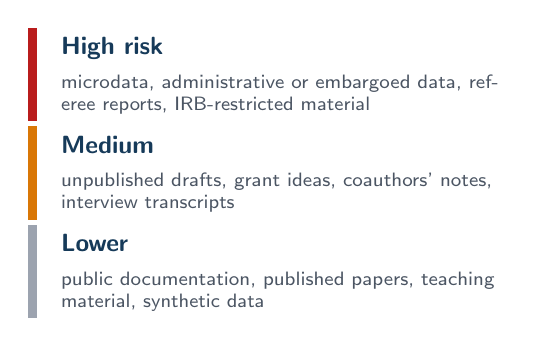
\begin{tikzpicture}[y=-1.25cm]
        \foreach \i/\lvl/\ex/\c in {%
          0/High risk/{microdata, administrative or embargoed data, referee reports, IRB-restricted material}/bad,%
          1/Medium/{unpublished drafts, grant ideas, coauthors' notes, interview transcripts}/accent,%
          2/Lower/{public documentation, published papers, teaching material, synthetic data}/faint}{%
          \fill[\c] (0,\i) rectangle ++(0.12,0.95);
          \node[anchor=north west,font=\small\bfseries,text=ink] at (0.3,\i) {\lvl};
          \node[anchor=north west,font=\scriptsize,text=muted,text width=5.6cm] at (0.3,\i+0.38) {\ex};
        }
      \end{tikzpicture}
    \column{0.44\textwidth}
      {\small
      \group{Whether it trains depends on}
      {\color{muted}the plan (consumer or business), the workspace settings, the API retention policy, and every tool the agent calls on the way.\par}
      \vspace{0.8em}
      {\color{ink}\bfseries Settings change. Check them; do not assume them.\par}
      \vspace{0.8em}
      {\color{muted}When in doubt: anonymise, use a synthetic copy, or run locally.\par}}
  \end{columns}
\end{frame}

% -------- Reliability words --------
\begin{frame}{Reliability words you will keep hearing}
  \vspace{0.4em}
  \begin{center}
  \renewcommand{\arraystretch}{1.25}
  \begin{tabularx}{0.9\linewidth}{>{\bfseries\color{ink}}l X}
  \toprule
  Hallucination & a confident output with no basis: a citation, a number, a variable\\
  Context rot & quality falls as the context window fills\\
  Reward hacking & the agent meets the check and misses the goal, for example by editing the test instead of the code\\
  Sycophancy & the model agrees with you when you are wrong\\
  Automation bias & we trust automated output more than it deserves \citep{skitka_1999_automation_bias}\\
  Drift & the same prompt gives different results after a model update\\
  \bottomrule
  \end{tabularx}
  \end{center}
  \takeaway{Lesson 3 is about controlling all six.}
\end{frame}

% =============================================================
% Closing: glossary, homework, references
% =============================================================

% -------- Twelve words, one line each --------
\begin{frame}{Twelve words, one line each}
  \vspace{0.3em}
  \begin{columns}[T,onlytextwidth]
    \column{0.31\textwidth}
      \group{What an agent is}
      {\footnotesize
      \textbf{\color{ink}Model}: the network that predicts text.\\[0.45em]
      \textbf{\color{ink}Harness}: the runtime around it: loop, tools, context, controls.\\[0.45em]
      \textbf{\color{ink}Agent}: model plus harness, given a task.\\[0.45em]
      \textbf{\color{ink}Tool and permission}: what it can call, and what it may do without asking.\par}
    \column{0.31\textwidth}
      \group{What it sees}
      {\footnotesize
      \textbf{\color{ink}Prompt}: one request, one answer.\\[0.45em]
      \textbf{\color{ink}Context window}: everything the model sees in one turn.\\[0.45em]
      \textbf{\color{ink}Token}: the unit it reads, writes and bills.\\[0.45em]
      \textbf{\color{ink}Compaction}: old turns replaced by a summary when the window fills.\par}
    \column{0.31\textwidth}
      \group{How you extend it}
      {\footnotesize
      \textbf{\color{ink}Rules file}: instructions loaded at every start, such as \texttt{AGENTS.md}.\\[0.45em]
      \textbf{\color{ink}MCP}: an open standard that plugs tools and data into a harness.\\[0.45em]
      \textbf{\color{ink}Skill}: a \texttt{SKILL.md} procedure loaded when a request matches.\\[0.45em]
      \textbf{\color{ink}Sub-agent}: a helper agent with its own context and one job.\par}
  \end{columns}
\end{frame}

% -------- Before Lesson 2 --------
\begin{frame}{Before Lesson 2}
  \vspace{1.2em}
  {\Large\color{ink}\bfseries Install one harness.\par}
  \vspace{0.3em}{\small\color{muted}ChatGPT desktop with Codex, Claude Code, Cursor or OpenCode.\par}
  \vspace{1.0em}
  {\Large\color{ink}\bfseries Connect one MCP server.\par}
  \vspace{0.3em}{\small\color{muted}Any one: a file system, your calendar, Stata.\par}
  \vspace{1.0em}
  {\Large\color{ink}\bfseries Write a ten-line \texttt{AGENTS.md} for a real project.\par}
  \vspace{0.3em}{\small\color{muted}Layout, what must not change, what ``done'' means. Bring it to Lesson 2.\par}
  \vfill
  {\color{muted}\scriptsize Demo repository: \url{https://github.com/MarcoLeMoglie/demo-lesson1}\par}
\end{frame}

% -------- References --------
\begin{frame}[allowframebreaks]{References}
  \nocite{*}
  \scriptsize
  \bibliography{lesson1/lesson1}
\end{frame}


\end{document}

\else\ifnum\CompileSession=2
  % =============================================================
% Session 2 — entry point (hours 3–4)
% Overleaf: Main document -> session2/session2.tex
% Output: session2.pdf
% =============================================================

% =============================================================
% Agentic AI for Economic Research -- Beamer custom theme
% Compiler: pdflatex (no fontspec)
% Marco Le Moglie, Catholic University of the Sacred Heart, 2026
% =============================================================

\documentclass[aspectratio=169,10pt]{beamer}

% ---------- Encoding and language ----------
\usepackage[T1]{fontenc}
\usepackage[utf8]{inputenc}
\usepackage[english]{babel}

% ---------- Modern sans-serif fonts (pdflatex-compatible) ----------
\usepackage[default,scale=0.95]{sourcesanspro}
\usepackage[scaled=0.85]{sourcecodepro}
\renewcommand{\familydefault}{\sfdefault}
\usepackage{microtype}

% ---------- Graphics and colour ----------
\usepackage{graphicx}
\usepackage{xcolor}
\usepackage{tikz}
\usetikzlibrary{positioning,arrows.meta,calc,shapes.geometric,fit,backgrounds,shadows.blur,decorations.pathreplacing}
\usepackage{pgfplots}
\pgfplotsset{compat=1.18}
\usepackage{tabularx}
\usepackage{booktabs}
\usepackage{array}
\usepackage{ragged2e}
\usepackage{hyperref}
\usepackage{fontawesome5}
\usepackage[most]{tcolorbox}
\usepackage[round,authoryear]{natbib}
\bibliographystyle{plainnat}

\graphicspath{{assets/}{assets/real/}{assets/charts/}{assets/icons/}{assets/legacy/}}

\hypersetup{colorlinks=true,linkcolor=deepblue,urlcolor=accent,citecolor=deepblue}

% ---------- Palette ----------
\definecolor{deepblue}{HTML}{163A59}
\definecolor{accent}{HTML}{D97706}
\definecolor{softblue}{HTML}{EAF3FF}
\definecolor{softorange}{HTML}{FFF4E6}
\definecolor{softgreen}{HTML}{EAF8EF}
\definecolor{softpurple}{HTML}{F2ECFA}
\definecolor{softgray}{HTML}{F3F4F6}
\definecolor{dark}{HTML}{111827}
\definecolor{muted}{HTML}{4B5563}
\definecolor{good}{HTML}{166534}
\definecolor{bad}{HTML}{B91C1C}

% ---------- Beamer base look (custom theme, no metropolis) ----------
\useinnertheme{rectangles}
\useoutertheme{default}
\setbeamersize{text margin left=1.2em,text margin right=1.2em}

\setbeamercolor{normal text}{fg=dark,bg=white}
\setbeamercolor{structure}{fg=deepblue}
\setbeamercolor{alerted text}{fg=accent}

% Frametitle: a thin coloured bar with title in deep blue, no background block
\setbeamerfont{frametitle}{size=\Large,series=\bfseries}
\setbeamercolor{frametitle}{fg=deepblue,bg=white}
\setbeamertemplate{frametitle}{%
  \vspace{0.4em}%
  \begin{minipage}[t]{\dimexpr\paperwidth-2.4em\relax}%
    \raggedright\insertframetitle\par
    \vspace{-0.25em}%
    {\color{accent}\rule{2.6em}{1.4pt}}%
  \end{minipage}%
  \vspace{0.1em}%
}

% Footline: discrete page number and short course tag
\setbeamertemplate{navigation symbols}{}
\setbeamertemplate{footline}{%
  \leavevmode%
  \hbox{%
    \begin{beamercolorbox}[wd=.6\paperwidth,ht=2.2ex,dp=1ex,leftskip=1em]{footline}%
      \usebeamerfont{author in head/foot}\color{muted}\scriptsize Agentic AI for Economic Research\,\textbar\,Marco Le Moglie\,\textbar\,Cattolica%
    \end{beamercolorbox}%
    \begin{beamercolorbox}[wd=.4\paperwidth,ht=2.2ex,dp=1ex,rightskip=1em,leftskip=1em]{footline}%
      \usebeamerfont{author in head/foot}\hfill\color{muted}\scriptsize\insertframenumber\,/\,\inserttotalframenumber%
    \end{beamercolorbox}%
  }%
}

% Items
\setbeamertemplate{itemize item}{\color{accent}\faChevronRight}
\setbeamertemplate{itemize subitem}{\color{deepblue}\faCircle}
\setbeamercolor{itemize item}{fg=accent}
\setbeamercolor{itemize subitem}{fg=deepblue}

% ---------- Custom commands ----------
\newcommand{\smallsource}[1]{\vfill{\scriptsize\color{muted}\itshape Source: #1\par}}
\newcommand{\srcfoot}[1]{{\scriptsize\color{muted}\itshape #1}}
\newcommand{\bigpoint}[1]{\begin{center}\Huge\bfseries\color{deepblue}#1\end{center}}
\newcommand{\midpoint}[1]{\begin{center}\Large\bfseries\color{deepblue}#1\end{center}}
\newcommand{\alertbox}[1]{%
  \begin{tcolorbox}[colback=softorange,colframe=accent,arc=2pt,boxrule=0.6pt]%
    #1%
  \end{tcolorbox}%
}

% Two-/three-bullet shortcuts
\newcommand{\twobullets}[2]{\begin{itemize}\setlength\itemsep{0.4em}\item #1\item #2\end{itemize}}
\newcommand{\threebullets}[3]{\begin{itemize}\setlength\itemsep{0.4em}\item #1\item #2\item #3\end{itemize}}
\newcommand{\fourbullets}[4]{\begin{itemize}\setlength\itemsep{0.35em}\item #1\item #2\item #3\item #4\end{itemize}}

% Section divider (full-bleed coloured frame)
\newcommand{\sectionframe}[2][deepblue]{%
\begin{frame}[plain]
  \begin{tikzpicture}[remember picture,overlay]
    \fill[#1] (current page.south west) rectangle (current page.north east);
    \node[anchor=south west,inner sep=1.3cm,text=white,align=left,text width=0.85\paperwidth] at (current page.south west){\fontsize{30}{36}\selectfont\bfseries #2};
    \node[anchor=north east,inner sep=1.0cm,text=accent] at (current page.north east){\rule{4cm}{2pt}};
  \end{tikzpicture}
\end{frame}}

% Image-only frame with optional caption
\newcommand{\imageonly}[3][0.86]{%
\begin{frame}{#2}
  \begin{center}
    \includegraphics[width=#1\linewidth,height=0.7\textheight,keepaspectratio]{#3}
  \end{center}
\end{frame}}

% Title-as-question variant
\newcommand{\question}[1]{\begin{center}\LARGE\bfseries\color{deepblue}#1\end{center}}

% ---------- Document metadata ----------
\title{Agentic AI for Economic Research}
\subtitle{Concepts, tools, workflows and responsible use}
\author{Marco Le Moglie\\\small Catholic University of the Sacred Heart}
\institute{Agentic Economic Research}
\date{\today}


\setbeamertemplate{footline}{%
  \leavevmode%
  \hbox{%
    \begin{beamercolorbox}[wd=.6\paperwidth,ht=2.2ex,dp=1ex,leftskip=1em]{footline}%
      \usebeamerfont{author in head/foot}\color{muted}\scriptsize Agentic AI for Economic Research\,\textbar\,Session 2\,\textbar\,Marco Le Moglie\,\textbar\,Cattolica%
    \end{beamercolorbox}%
    \begin{beamercolorbox}[wd=.4\paperwidth,ht=2.2ex,dp=1ex,rightskip=1em,leftskip=1em]{footline}%
      \usebeamerfont{author in head/foot}\hfill\color{muted}\scriptsize\insertframenumber\,/\,\inserttotalframenumber%
    \end{beamercolorbox}%
  }%
}

\begin{document}

% =============================================================
% Session 2 -- Block 0: Opening and today's roadmap
% Title -- What we see today (overview) -- Four parts in detail
% =============================================================

% -------- Slide 1: Title (full-bleed) --------
\begin{frame}[plain]
  \begin{tikzpicture}[remember picture,overlay]
    \fill[deepblue] (current page.south west) rectangle (current page.north east);
    \fill[accent,opacity=0.85]
      ($(current page.south east)+(-6,0)$) --
      ($(current page.south east)+(0,0)$) --
      ($(current page.south east)+(0,3.2)$) -- cycle;
    \node[anchor=north west,inner sep=1.3cm,text=white,align=left,text width=0.86\paperwidth] at (current page.north west){%
      {\fontsize{34}{40}\selectfont\bfseries Agentic AI for\\Economic Research}\\[0.35cm]
      {\Large Session 2: live workflows, case studies, and lessons learned}\\[1.0cm]
      {\large\bfseries Marco Le Moglie}\\[0.05cm]
      {\normalsize Catholic University of the Sacred Heart}\\[0.5cm]
      {\small Agentic Economic Research seminar\,\textbar\,Session 2}\\[0.05cm]
      {\small Mini-course for PhD students and faculty\,\textbar\,hours 3--4}\\[0.12cm]
      {\footnotesize\href{https://github.com/MarcoLeMoglie/Agentic_Economic_Research}{\textcolor{white}{Slides source on GitHub}}}};
  \end{tikzpicture}
\end{frame}

% -------- Slide 2: What we see today (four-part overview) --------
\begin{frame}{What we see today}
  \vspace{0.15cm}
  \begin{center}
  \begin{tikzpicture}[
    node distance=0.55cm and 0.5cm,
    every node/.style={align=left,font=\small},
    part/.style={draw=deepblue,fill=softblue,rounded corners,very thick,
      minimum width=6.8cm,minimum height=1.05cm,text width=6.5cm,inner sep=6pt}
  ]
    \node[part] (p1) {\textbf{1. Agent interfaces}\quad\scriptsize live screens};
    \node[part,below=of p1] (p2) {\textbf{2. Success stories}\quad\scriptsize projects at equilibrium};
    \node[part,below=of p2] (p3) {\textbf{3. Second brain}\quad\scriptsize Obsidian vault \& memory};
    \node[part,below=of p3] (p4) {\textbf{4. Work in progress}\quad\scriptsize live screens};
    \node[anchor=west,right=0.9cm of p1,text width=5.8cm,font=\scriptsize,color=muted] (n1)
      {Chat, desktop apps, IDE, CLI --- menus and options in real tools.};
    \node[anchor=west,right=0.9cm of p2,text width=5.8cm,font=\scriptsize,color=muted] (n2)
      {Selected projects where the agent workflow is clean and repeatable.};
    \node[anchor=west,right=0.9cm of p3,text width=5.8cm,font=\scriptsize,color=muted] (n3)
      {How it works; how I organise mine; how you might organise yours.};
    \node[anchor=west,right=0.9cm of p4,text width=5.8cm,font=\scriptsize,color=muted] (n4)
      {Bootstrap, supervision, errors --- all on real screens.};
  \end{tikzpicture}
  \end{center}
 
\end{frame}

% -------- Slide 3: Part 1 -- Interfaces (detail) --------
\sectionframe[deepblue]{Part 1 -- Agent interfaces}

\begin{frame}{Part 1: four interface families, live}
  \begin{columns}[T,onlytextwidth]
    \column{0.48\textwidth}
      \textbf{Today we open the real tools}
      \begin{itemize}\setlength\itemsep{0.45em}
        \item \textbf{Chat window}
        \item \textbf{Desktop agent apps} 
        \item \textbf{IDE agents} 
        \item \textbf{CLI in the terminal} 
      \end{itemize}
    \column{0.48\textwidth}
      \alertbox{%
        \textbf{Live demo goal}\\[0.2em]
        Not a feature tour for its own sake: show \emph{where} autonomy lives in each interface --- and which menu choices matter for research.%
      }
    
  \end{columns}
\end{frame}

% -------- Slide 4: Part 2 -- Success stories (overview) --------
\sectionframe[deepblue]{Part 2 -- Success stories}

\begin{frame}{Part 2: projects at equilibrium}
  \small
  \textbf{For each case: objective, current workflow, what we learned, problems hit.}
  \vspace{0.35cm}
  \begin{columns}[T,onlytextwidth]
    \column{0.48\textwidth}
      \begin{itemize}\setlength\itemsep{0.32em}
        \item \textbf{YouTube channel} --- economics explainer pipeline.
        \item \textbf{Newsletter} --- ASSIST Weekly harvest-to-send stack.
        \item \textbf{Mafia culture} --- datasets, reports, documentation agents.
      \end{itemize}
    \column{0.48\textwidth}
      \begin{itemize}\setlength\itemsep{0.32em}
        \item \textbf{Paper review} --- referee-report skills and adversarial checks.
        \item \textbf{Purge} --- journal-target skill adapted to a new outlet.
      \end{itemize}
  \end{columns}
  \vspace{0.35cm}
  \begin{center}{\color{deepblue}\bfseries Common thread: repeatable folder discipline + human gates.}\end{center}
\end{frame}

% =============================================================
% Session 2 -- Block 2 (detail): Success stories — one slide per project
% =============================================================

% -------- Success story: YouTube channel --------
\begin{frame}{Success story: \emph{Cosa fanno gli Economisti}}
  \footnotesize
  \textbf{Live links:}
  \href{https://www.youtube.com/@cosafannoglieconomisti26}{YouTube}
  \,\textbar\,
  \href{https://www.instagram.com/cosafannoglieconomisti}{Instagram}
  \,\textbar\,
  \href{https://www.facebook.com/cosafannoglieconomisti}{Facebook}
  \vspace{0.15cm}
  \begin{columns}[T,onlytextwidth]
    \column{0.48\textwidth}
      \textbf{Objective}
      \begin{itemize}\setlength\itemsep{0.2em}
        \item Turn economics papers into short explainer videos for a general audience.
        \item Automate production, SEO, YouTube programming, and cross-posting (FB/IG).
      \end{itemize}
      \vspace{0.15cm}
      \textbf{Current state \& workflow}
      \begin{itemize}\setlength\itemsep{0.2em}
        \item End-to-end: paper $\rightarrow$ cover $\rightarrow$ NotebookLM video $\rightarrow$ cleanup $\rightarrow$ multilingual upload $\rightarrow$ Buffer social.
        \item \textbf{Codex chat} = control plane; runner \texttt{./workflow} + scripts in \texttt{Execution/}.
        \item Three layers: \emph{Directives} (SOP) $\rightarrow$ orchestration $\rightarrow$ deterministic execution.
        \item Lanes: Enea (production), Romolo (YouTube/SEO), Marcello (social), Mercurio (backup), Ulisse (scouting).
      \end{itemize}
    \column{0.48\textwidth}
      \textbf{What I learned}
      \begin{itemize}\setlength\itemsep{0.2em}
        \item \textbf{Connectors}: MCP (NotebookLM), APIs (YouTube, Buffer), CLI (\texttt{nlm}, \texttt{./workflow}).
        \item \textbf{Structured rules} + \textbf{multi-agent} workflows; truth in \texttt{video\_tracking.json}.
        \item \textbf{Token control}: targeted git push, recover partial uploads, no blind re-runs.
        \item \textbf{YouTube SEO}: titles, playlists, competitor comments, monthly report.
        \item \textbf{Tool drift}: Antigravity/Codex upgrades broke rules, MCP paths, terminal defaults --- re-audit SOPs after each version jump.
      \end{itemize}
      \vspace{0.1cm}
      \textbf{Problems hit}
      \begin{itemize}\setlength\itemsep{0.2em}
        \item Buffer 404 until assets on GitHub; NotebookLM MCP vs.\ CLI cookie mismatch.
        \item YouTube thumbnail $>$2\,MB after upload; Telegram retired $\rightarrow$ Codex-first.
      \end{itemize}
  \end{columns}
\end{frame}

% -------- Success story: ASSIST Weekly newsletter --------
\begin{frame}[t]{Success story: \emph{ASSIST Weekly} (newsletter)}
  \tiny
  \textbf{Live link:} \href{https://www.assistweekly.org/}{assistweekly.org}
  \vspace{0.08cm}
  \begin{columns}[T,onlytextwidth]
    \column{0.48\textwidth}
      \textbf{Objective}
      \begin{itemize}\setlength\itemsep{0.1em}
        \item Weekly brief: datasets, tools/methods, working papers.
        \item Stack: discover $\rightarrow$ QA $\rightarrow$ email $\rightarrow$ landing/signup.
      \end{itemize}
      \textbf{Current state}
      \begin{itemize}\setlength\itemsep{0.1em}
        \item \#13 sent 2026-07-06; \texttt{2026-07-13} shortlist ready.
        \item Brevo campaigns; Cloudflare Pages/Worker; internal dashboard.
      \end{itemize}
      \textbf{Three automations}
      \begin{itemize}\setlength\itemsep{0.08em}
        \item \textbf{Wed} harvest $\rightarrow$ shortlist + dashboard
        \item \textbf{Thu} render after \texttt{APPROVED.flag}
        \item \textbf{Mon} Brevo send after \texttt{EMAIL\_APPROVED}
      \end{itemize}
      {\scriptsize\color{muted}Manual gates: dashboard review $\rightarrow$ flags.}
    \column{0.48\textwidth}
      \textbf{What I learned}
      \begin{itemize}\setlength\itemsep{0.1em}
        \item Brevo; Cloudflare deploy; editorial dashboard.
        \item Scraping/APIs (GitHub, Dataverse, NBER, CEPR).
        \item Brand/trademark; anti-slop frontend; LaunchAgents.
      \end{itemize}
      \textbf{Problems hit}
      \begin{itemize}\setlength\itemsep{0.1em}
        \item Source selection \& over-harvest filters.
        \item Manual ratings train judgment between automations.
      \end{itemize}
  \end{columns}
\end{frame}

% -------- Success story: Mafia Culture / Neomelodic Corpus --------
\begin{frame}[t]{Success story: \emph{Mafia Culture} (Neomelodic Corpus)}
  \scriptsize
  \textbf{Repo:} \href{https://github.com/MarcoLeMoglie/Mafia_culture}{github.com/MarcoLeMoglie/Mafia\_culture}
  \vspace{0.06cm}
  \begin{columns}[T,onlytextwidth]
    \column{0.56\textwidth}
      \textbf{Objective}
      \begin{itemize}\setlength\itemsep{0.08em}
        \item Build a reproducible corpus of Italian neomelodic music (artists, tracks, lyrics) for cultural economics.
      \end{itemize}
      \textbf{Current state}
      \begin{itemize}\setlength\itemsep{0.08em}
        \item \textbf{190} artists; \textbf{32.5k} title-level tracks; \textbf{2.6k} high-confidence lyrics in reports.
        \item Four LaTeX PDF reports (links $\rightarrow$); canonical layers in \texttt{analysis/}.
      \end{itemize}
      \textbf{Pilot corpus steps} (legacy pipeline)
      \begin{itemize}\setlength\itemsep{0.06em}
        \item Seed artists $\rightarrow$ metadata harvest $\rightarrow$ dedup export $\rightarrow$ Stata layers $\rightarrow$ standardized PDF reports.
      \end{itemize}
      \textbf{Spotify frontier} (vs.\ core artist seeds)
      \begin{itemize}\setlength\itemsep{0.06em}
        \item \texttt{seed-core} (190) $\rightarrow$ \texttt{discover-network} $\rightarrow$ \texttt{sync-mirror} $\rightarrow$ LRCLib lyrics $\rightarrow$ Jaccard export.
        \item Goal: full discographies + audio features beyond the original artist list.
      \end{itemize}
      \textbf{What I learned}
      \begin{itemize}\setlength\itemsep{0.06em}
        \item \textbf{Machine generates, human verifies}: sample construction + exploratory QA loops.
        \item \textbf{Standardized LaTeX reports} as control documents; branch + commit at each dataset decision.
        \item \textbf{Cold-start replication package} when a layer is ``ready''.
      \end{itemize}
    \column{0.42\textwidth}
      \centering
      
\includegraphics[width=\linewidth,height=0.34\textheight,keepaspectratio]{mafia-culture/wc_tracks_malavita.png}\\[0.08cm]
      {\scriptsize\color{muted}Tracks report --- malavita word cloud}\\[0.12cm]
      \textbf{Report PDFs}\\[0.06cm]
      \href{assets/mafia-culture/reports/corpus.pdf}{Corpus}\,\textbar\,
      \href{assets/mafia-culture/reports/artists.pdf}{Artists}\,\textbar\,
      \href{assets/mafia-culture/reports/tracks.pdf}{Tracks}\,\textbar\,
      \href{assets/mafia-culture/reports/lyrics.pdf}{Lyrics}
      \vspace{0.1cm}
      \textbf{Problems hit}
      \begin{itemize}\setlength\itemsep{0.06em}
        \item Layer drift (raw vs.\ canonical vs.\ compatibility surfaces).
        \item Spotify API limits, album dedup, partial lyrics coverage ($\sim$20--40\%).
      \end{itemize}
  \end{columns}
\end{frame}

% =============================================================
% Session 2 -- Success stories (extra slides) — append only
% =============================================================

% -------- Success story: Paper peer review (/referaggio skill) --------
\begin{frame}[t]{Success story: Skill \texttt{/referee-report}}
  \footnotesize
  \textbf{Objective:} turn an annotated manuscript into a constructive English referee report in Marco's voice, with adversarial checks and style archive.
  \vspace{0.2cm}
  \begin{columns}[T,onlytextwidth]
    \column{0.48\textwidth}
      \textbf{Skill \texttt{/referaggio} --- main steps}
      \begin{enumerate}\setlength\itemsep{0.18em}
        \item \textbf{Intake} --- Marco uploads annotated PDF to \texttt{reviews/}.
        \item \textbf{Scaffold} --- folder \texttt{\{MS-ID\}-\{JOURNAL\}/} + checklist.
        \item \textbf{Comments} --- extract, expand, organize; drop nonsense \emph{with reason}.
        \item \textbf{Econoclast} --- adversarial pass; \alert{manual PDF verify} each finding.
        \item \textbf{Plan} --- \texttt{proposed\_points.md}; \alert{STOP: Marco approves}.
        \item \textbf{Draft} --- \texttt{referee\_report.tex/md/pdf} (conciliatory tone).
        \item \textbf{Anti-slop} --- \texttt{prose-check} on draft.
        \item \textbf{Archive} --- style example; \alert{STOP: final Marco approval}.
      \end{enumerate}
    \column{0.48\textwidth}
      \alertbox{%
        \textbf{Human gates (non-negotiable)}\\[0.15em]
        \scriptsize
        Wait for PDF upload (step 1). Clarify ambiguous comments (step 3). Approve integrated plan before drafting (step 5). Approve final report before archive (step 8). Econoclast supplements --- does not replace Marco's judgment.%
      }
    
  \end{columns}
\end{frame}

% -------- Success story: Purge --- journal-style-paper-rewrite skill --------
\begin{frame}[t]{Success story: Skill \texttt{/journal-style-paper-rewrite}}
  \footnotesize
  \textbf{Objective:} adapt a frozen paper (e.g.\ J. Popul. Econ.$\rightarrow$ Demography) --- new framing and prose, \emph{same} empirical package.
  \vspace{0.15cm}
  \begin{columns}[T,onlytextwidth]
    \column{0.48\textwidth}
      \textbf{Skill workflow --- main parts}
      \begin{enumerate}\setlength\itemsep{0.16em}
        \item \textbf{Lock source} --- read memory; \alert{do not edit frozen paper}.
        \item \textbf{Preserve empirics} --- no new regressions/tables unless Marco reopens.
        \item \textbf{Design prompt} --- \alert{ask Marco if missing} (journal, framing, tone).
        \item \textbf{Target-journal plan} --- title/abstract, intro, results rhetoric.
        \item \textbf{Anti-slop} --- prose-check on new version.
        \item \textbf{Two outputs} --- \texttt{AA\_paper\_<journal>.tex} + matching report.
        \item \textbf{Color logic} --- mark only text actually changed vs.\ source.
        \item \textbf{Compile \& verify} --- source untouched; report matches new version.
      \end{enumerate}
    \column{0.48\textwidth}
      \alertbox{%
        \textbf{Human gates}\\[0.15em]
        \scriptsize
        Frozen paper stays read-only. Journal-design prompt required before any rewrite. Marco approves framing; agents do not improvise empirical reopening. Color only real edits%
      }
     
  \end{columns}
\end{frame}


\end{document}

\else
  % =============================================================
% Session 1 — entry point (hours 1–2)
% Overleaf: Main document -> session1/session1.tex
% Output: session1.pdf
% =============================================================

% =============================================================
% Agentic AI for Economic Research -- Beamer custom theme
% Compiler: pdflatex (no fontspec)
% Marco Le Moglie, Catholic University of the Sacred Heart, 2026
% =============================================================

\documentclass[aspectratio=169,10pt]{beamer}

% ---------- Encoding and language ----------
\usepackage[T1]{fontenc}
\usepackage[utf8]{inputenc}
\usepackage[english]{babel}

% ---------- Modern sans-serif fonts (pdflatex-compatible) ----------
\usepackage[default,scale=0.95]{sourcesanspro}
\usepackage[scaled=0.85]{sourcecodepro}
\renewcommand{\familydefault}{\sfdefault}
\usepackage{microtype}

% ---------- Graphics and colour ----------
\usepackage{graphicx}
\usepackage{xcolor}
\usepackage{tikz}
\usetikzlibrary{positioning,arrows.meta,calc,shapes.geometric,fit,backgrounds,shadows.blur,decorations.pathreplacing}
\usepackage{pgfplots}
\pgfplotsset{compat=1.18}
\usepackage{tabularx}
\usepackage{booktabs}
\usepackage{array}
\usepackage{ragged2e}
\usepackage{hyperref}
\usepackage{fontawesome5}
\usepackage[most]{tcolorbox}
\usepackage[round,authoryear]{natbib}
\bibliographystyle{plainnat}

\graphicspath{{assets/}{assets/real/}{assets/charts/}{assets/icons/}{assets/legacy/}}

\hypersetup{colorlinks=true,linkcolor=deepblue,urlcolor=accent,citecolor=deepblue}

% ---------- Palette ----------
\definecolor{deepblue}{HTML}{163A59}
\definecolor{accent}{HTML}{D97706}
\definecolor{softblue}{HTML}{EAF3FF}
\definecolor{softorange}{HTML}{FFF4E6}
\definecolor{softgreen}{HTML}{EAF8EF}
\definecolor{softpurple}{HTML}{F2ECFA}
\definecolor{softgray}{HTML}{F3F4F6}
\definecolor{dark}{HTML}{111827}
\definecolor{muted}{HTML}{4B5563}
\definecolor{good}{HTML}{166534}
\definecolor{bad}{HTML}{B91C1C}

% ---------- Beamer base look (custom theme, no metropolis) ----------
\useinnertheme{rectangles}
\useoutertheme{default}
\setbeamersize{text margin left=1.2em,text margin right=1.2em}

\setbeamercolor{normal text}{fg=dark,bg=white}
\setbeamercolor{structure}{fg=deepblue}
\setbeamercolor{alerted text}{fg=accent}

% Frametitle: a thin coloured bar with title in deep blue, no background block
\setbeamerfont{frametitle}{size=\Large,series=\bfseries}
\setbeamercolor{frametitle}{fg=deepblue,bg=white}
\setbeamertemplate{frametitle}{%
  \vspace{0.4em}%
  \begin{minipage}[t]{\dimexpr\paperwidth-2.4em\relax}%
    \raggedright\insertframetitle\par
    \vspace{-0.25em}%
    {\color{accent}\rule{2.6em}{1.4pt}}%
  \end{minipage}%
  \vspace{0.1em}%
}

% Footline: discrete page number and short course tag
\setbeamertemplate{navigation symbols}{}
\setbeamertemplate{footline}{%
  \leavevmode%
  \hbox{%
    \begin{beamercolorbox}[wd=.6\paperwidth,ht=2.2ex,dp=1ex,leftskip=1em]{footline}%
      \usebeamerfont{author in head/foot}\color{muted}\scriptsize Agentic AI for Economic Research\,\textbar\,Marco Le Moglie\,\textbar\,Cattolica%
    \end{beamercolorbox}%
    \begin{beamercolorbox}[wd=.4\paperwidth,ht=2.2ex,dp=1ex,rightskip=1em,leftskip=1em]{footline}%
      \usebeamerfont{author in head/foot}\hfill\color{muted}\scriptsize\insertframenumber\,/\,\inserttotalframenumber%
    \end{beamercolorbox}%
  }%
}

% Items
\setbeamertemplate{itemize item}{\color{accent}\faChevronRight}
\setbeamertemplate{itemize subitem}{\color{deepblue}\faCircle}
\setbeamercolor{itemize item}{fg=accent}
\setbeamercolor{itemize subitem}{fg=deepblue}

% ---------- Custom commands ----------
\newcommand{\smallsource}[1]{\vfill{\scriptsize\color{muted}\itshape Source: #1\par}}
\newcommand{\srcfoot}[1]{{\scriptsize\color{muted}\itshape #1}}
\newcommand{\bigpoint}[1]{\begin{center}\Huge\bfseries\color{deepblue}#1\end{center}}
\newcommand{\midpoint}[1]{\begin{center}\Large\bfseries\color{deepblue}#1\end{center}}
\newcommand{\alertbox}[1]{%
  \begin{tcolorbox}[colback=softorange,colframe=accent,arc=2pt,boxrule=0.6pt]%
    #1%
  \end{tcolorbox}%
}

% Two-/three-bullet shortcuts
\newcommand{\twobullets}[2]{\begin{itemize}\setlength\itemsep{0.4em}\item #1\item #2\end{itemize}}
\newcommand{\threebullets}[3]{\begin{itemize}\setlength\itemsep{0.4em}\item #1\item #2\item #3\end{itemize}}
\newcommand{\fourbullets}[4]{\begin{itemize}\setlength\itemsep{0.35em}\item #1\item #2\item #3\item #4\end{itemize}}

% Section divider (full-bleed coloured frame)
\newcommand{\sectionframe}[2][deepblue]{%
\begin{frame}[plain]
  \begin{tikzpicture}[remember picture,overlay]
    \fill[#1] (current page.south west) rectangle (current page.north east);
    \node[anchor=south west,inner sep=1.3cm,text=white,align=left,text width=0.85\paperwidth] at (current page.south west){\fontsize{30}{36}\selectfont\bfseries #2};
    \node[anchor=north east,inner sep=1.0cm,text=accent] at (current page.north east){\rule{4cm}{2pt}};
  \end{tikzpicture}
\end{frame}}

% Image-only frame with optional caption
\newcommand{\imageonly}[3][0.86]{%
\begin{frame}{#2}
  \begin{center}
    \includegraphics[width=#1\linewidth,height=0.7\textheight,keepaspectratio]{#3}
  \end{center}
\end{frame}}

% Title-as-question variant
\newcommand{\question}[1]{\begin{center}\LARGE\bfseries\color{deepblue}#1\end{center}}

% ---------- Document metadata ----------
\title{Agentic AI for Economic Research}
\subtitle{Concepts, tools, workflows and responsible use}
\author{Marco Le Moglie\\\small Catholic University of the Sacred Heart}
\institute{Agentic Economic Research}
\date{\today}


\begin{document}

% =============================================================
% Block 0 -- Opening (3 slides)
% Title -- Who I am / what this course is NOT -- Roadmap
% =============================================================

% -------- Slide 1: Title (full-bleed) --------
\begin{frame}[plain]
  \begin{tikzpicture}[remember picture,overlay]
    \fill[deepblue] (current page.south west) rectangle (current page.north east);
    % accent diagonal stripe in the bottom-right corner
    \fill[accent,opacity=0.85]
      ($(current page.south east)+(-6,0)$) --
      ($(current page.south east)+(0,0)$) --
      ($(current page.south east)+(0,3.2)$) -- cycle;
    \node[anchor=north west,inner sep=1.3cm,text=white,align=left,text width=0.86\paperwidth] at (current page.north west){%
      {\fontsize{34}{40}\selectfont\bfseries Agentic AI for\\Economic Research}\\[0.4cm]
      {\Large Concepts, tools, workflows and responsible use}\\[1.2cm]
      {\large\bfseries Marco Le Moglie}\\[0.05cm]
      {\normalsize Catholic University of the Sacred Heart}\\[0.6cm]
      {\small Agentic Economic Research seminar\,\textbar\,1 July 2026}\\[0.05cm]
       {\small Mini-course for PhD students and faculty\,\textbar\,4 hours}\\[0.12cm]
       {\footnotesize\href{https://github.com/MarcoLeMoglie/Agentic_Economic_Research}{\textcolor{white}{Slides source on GitHub}}}};
  \end{tikzpicture}
\end{frame}

% -------- Slide 2: Who I am + what this course is NOT --------
\begin{frame}{Who I am, and what this course is \emph{not}}
  \begin{columns}[T,onlytextwidth]
    \column{0.50\textwidth}
      \textbf{Who I am}
      \begin{itemize}\setlength\itemsep{0.35em}
        \item Applied economist, Catholic University of the Sacred Heart.
        \item Daily user of agentic AI inside a research workflow: papers, replication, grants, teaching.
        \item Not a CS researcher or an AI safety specialist.
      \end{itemize}
      \vspace{0.3cm}
      \textbf{Why this course exists}
      \begin{itemize}\setlength\itemsep{0.35em}
        \item Doctoral students and faculty keep asking the same questions about tools, costs, privacy, autonomy.
        \item Most online material is either advertising or alarmism.
      \end{itemize}
    \column{0.46\textwidth}
      \textbf{This course is \alert{not}}
      \begin{itemize}\setlength\itemsep{0.35em}
        \item A coding tutorial.
        \item A benchmark comparison of language models.
        \item A discussion of artificial general intelligence.
        \item A claim that agents will replace researchers.
      \end{itemize}
      \vspace{0.3cm}
      \textbf{It \emph{is}}
      \begin{itemize}\setlength\itemsep{0.35em}
        \item A practical map for using agents in economics research without losing scientific control.
      \end{itemize}
  \end{columns}
\end{frame}

% -------- Slide 3: Course roadmap (4 hours, 2 sessions) --------
\begin{frame}{Course roadmap: four hours, two sessions}
  \begin{center}
  \begin{tikzpicture}[node distance=0.6cm and 0.8cm,every node/.style={align=center}]
    % Session 1
    \node[draw=deepblue,fill=softblue,rounded corners,very thick,
          minimum width=3.6cm,minimum height=1.3cm,text width=3.3cm]
          (s1) {\textbf{Session 1 -- today}\\\small 2 hours\\\scriptsize concepts \& tools};
    % Session 2
    \node[draw=accent,fill=softorange,rounded corners,very thick,
          minimum width=3.6cm,minimum height=1.3cm,right=2.5cm of s1,
          text width=3.3cm]
          (s2) {\textbf{Session 2 -- next}\\\small 2 hours\\\scriptsize case studies from my work};
    \draw[->,line width=1.4pt,color=accent] (s1.east) -- (s2.west)
          node[midway,above,font=\scriptsize,color=muted]{builds on};
    % Session 1 content (below s1)
    \node[anchor=north,below=0.5cm of s1,align=left,text width=5.2cm,font=\small]
      (s1c){%
      \textbf{1.} What is an agent? Vocabulary.\\
      \textbf{2.} Four families of interfaces.\\
      \textbf{3.} Cost, privacy, governance.\\
      \textbf{4.} Reliability and control.\\
      \textbf{5.} Architecture: rules, memory, MCP, sub-agents.\\
      \textbf{6.} A teaser of the case studies.};
    % Session 2 content (below s2)
    \node[anchor=north,below=0.5cm of s2,align=left,text width=5.2cm,font=\small]
      (s2c){%
      \textbf{A.} Literature review.\\
      \textbf{B.} Data and codebook documentation.\\
      \textbf{C.} Stata / R / Python debugging.\\
      \textbf{D.} Tables, robustness, specification curves.\\
      \textbf{E.} Referee reports, grants, teaching prep.};
  \end{tikzpicture}
  \end{center}
  \vspace{0.2cm}
  \midpoint{A practical map, not a technical manual.}
\end{frame}

% =============================================================
% Block 1 -- Why now (4 slides)
% From answering to acting -- Adoption chart -- What changed vs 2023 --
% Economists specifically
% =============================================================

\sectionframe{Part 1 -- Why now}

% -------- Slide 1: From answering to acting --------
\begin{frame}{From answering to acting}
  \begin{columns}[T,onlytextwidth]
    \column{0.50\textwidth}
      \threebullets%
        {AI is moving from \textbf{answering questions} to \textbf{taking actions}.}%
        {Research work is full of repeatable tasks: searching, coding, checking, documenting.}%
        {The hard question is no longer ``can it help?'' but \textbf{where should we trust it?}}
      \vspace{0.5cm}
      \midpoint{Agents change what we delegate.}
    \column{0.46\textwidth}
      \begin{tikzpicture}[font=\small,every node/.style={align=center}]
        \node[draw=deepblue,fill=softblue,rounded corners,very thick,
              minimum width=4cm,minimum height=1.05cm,text width=3.8cm]
              (chat){\textbf{2022--2023}\\Chatbots\\\scriptsize answer a prompt};
        \node[draw=accent,fill=softorange,rounded corners,very thick,
              minimum width=4cm,minimum height=1.05cm,text width=3.8cm,
              below=0.5cm of chat]
              (asst){\textbf{2023--2024}\\Assistants\\\scriptsize browse, read files};
        \node[draw=deepblue,fill=softgreen,rounded corners,very thick,
              minimum width=4cm,minimum height=1.05cm,text width=3.8cm,
              below=0.5cm of asst]
              (agent){\textbf{2024--2026}\\Agents\\\scriptsize plan, call tools, iterate};
        \draw[->,very thick,color=accent] (chat.south) -- (asst.north);
        \draw[->,very thick,color=accent] (asst.south) -- (agent.north);
      \end{tikzpicture}
  \end{columns}
\end{frame}

% -------- Slide 2: Adoption chart (researchers using AI) --------
\begin{frame}{Adoption among researchers is no longer marginal}
  \begin{columns}[T,onlytextwidth]
    \column{0.55\textwidth}
      \begin{tikzpicture}
        \begin{axis}[
            width=7.2cm,height=4.4cm,
            ybar,bar width=0.36cm,
            ymin=0,ymax=100,
            ylabel={\% researchers},
            ylabel style={font=\scriptsize,color=muted},
            xtick=data,
            xticklabels={2023 Nature\\survey,2024 Pew\\professionals,2025 Anthropic\\Economic Index},
            xticklabel style={align=center,font=\scriptsize},
            yticklabel style={font=\scriptsize,color=muted},
            ymajorgrids,grid style={dotted,gray!40},
            axis lines*=left,
            tick style={color=muted},
            enlarge x limits=0.30,
            nodes near coords,
            nodes near coords style={font=\scriptsize\bfseries,color=deepblue},
          ]
          \addplot[draw=deepblue,fill=deepblue!80,bar shift=-0.20cm]
            coordinates {(0,30) (1,55) (2,72)};
          \addplot[draw=accent,fill=accent!80,bar shift=0.20cm]
            coordinates {(0,8) (1,18) (2,36)};
        \end{axis}
      \end{tikzpicture}
      \vspace{0.1cm}\\
      {\scriptsize \color{deepblue}$\blacksquare$~any LLM use \quad \color{accent}$\blacksquare$~weekly use for work}
    \column{0.42\textwidth}
      \threebullets%
        {Roughly \textbf{1 in 3} researchers used an LLM at least once already in late 2023.}%
        {By 2025, surveys converge on a \textbf{majority} using LLMs at work and roughly \textbf{1 in 3} weekly.}%
        {The frontier is shifting from \emph{chat use} to \emph{agentic use} (tool calls, code, web).}
  \end{columns}
  \smallsource{Van Noorden \& Perkel, \emph{Nature} 2023; Pew Research 2024 survey of US professionals; Anthropic Economic Index \citeyearpar{anthropic_economic_index_2024} 2024--2025 update.}
\end{frame}

% -------- Slide 3: 3 novita vs ChatGPT 2023 --------
\begin{frame}{Three things that changed since ``ChatGPT 2023''}
  \vspace{0.2cm}
  \begin{center}
  \begin{tikzpicture}[every node/.style={align=center,font=\small}]
    \node[draw=deepblue,fill=softblue,rounded corners,very thick,
          minimum width=3.6cm,minimum height=2.3cm,text width=3.3cm]
          (tools){\textbf{1. Tools}\\\scriptsize browser, files, code, shell, search\\\scriptsize the model can \emph{do} things};
    \node[draw=accent,fill=softorange,rounded corners,very thick,
          minimum width=3.6cm,minimum height=2.3cm,text width=3.3cm,
          right=1.2cm of tools]
          (memory){\textbf{2. Memory}\\\scriptsize session, project, persistentency\\\scriptsize the model carries state};
    \node[draw=deepblue,fill=softgreen,rounded corners,very thick,
          minimum width=3.6cm,minimum height=2.3cm,text width=3.3cm,
          right=1.2cm of memory]
          (auto){\textbf{3. Autonomy}\\\scriptsize plan, loop, retry\\\scriptsize the model decides next steps};
  \end{tikzpicture}
  \end{center}
  \vspace{0.4cm}
  \midpoint{2023 was about \emph{generation}. 2025--2026 is about \emph{delegation}.}
\end{frame}

% -------- Slide 4: Why economists in particular --------
\begin{frame}{Why economists in particular should care}
  \begin{columns}[T,onlytextwidth]
    \column{0.48\textwidth}
      \textbf{Our work is unusually exposed.}
      \begin{itemize}\setlength\itemsep{0.3em}
        \item Heavy reading and writing.
        \item Long, fragile code pipelines.
        \item Tight reproducibility constraints.
        \item Long feedback loops with referees and coauthors.
      \end{itemize}
      \vspace{0.3cm}
      \textbf{Korinek's claim} \citep{korinek_jel_2023,korinek_2024_update}
      \begin{itemize}\setlength\itemsep{0.3em}
        \item LLMs already help across ideation, writing, code, math, data, and review.
        \item Agentic versions push the frontier from \emph{cognitive assist} to \emph{cognitive automation}.
      \end{itemize}
    \column{0.48\textwidth}
      \textbf{Brynjolfsson, Li, Raymond} \citep{brynjolfsson_aer_2025}
      \begin{itemize}\setlength\itemsep{0.3em}
        \item Productivity gains are concentrated on \textbf{less experienced workers}.
        \item Gains come from \emph{learned best practices}, not raw automation.
      \end{itemize}
      \vspace{0.3cm}
      \textbf{Implication for PhD training}
      \begin{itemize}\setlength\itemsep{0.3em}
        \item A young researcher who ignores agents loses a comparative advantage.
        \item A senior researcher who delegates without controls loses scientific control.
      \end{itemize}
  \end{columns}
\end{frame}

% =============================================================
% Block 2 -- Concepts and vocabulary (8 slides)
% Agent definition, chatbot vs agent, loop, prompt vs task,
% context/tokens, tools/permissions/sandbox, autonomy spectrum,
% reliability vocab.
% =============================================================

\sectionframe[accent]{Part 2 -- Concepts and vocabulary}

% -------- Slide 1: What is an agent? --------
\begin{frame}{What is an agent?}
  \begin{columns}[T,onlytextwidth]
    \column{0.46\textwidth}
      \bigpoint{LLM + tools\\+ goal + loop}
      \vspace{0.5cm}
      \begin{center}\color{muted}\small An agent is not a smarter chatbot.\\It is a workflow with partial autonomy.\end{center}
    \column{0.50\textwidth}
      \begin{tikzpicture}[every node/.style={align=center,font=\small}]
        \node[draw=deepblue,fill=softblue,rounded corners,very thick,
              minimum width=2.4cm,minimum height=0.9cm]
              (llm){\textbf{LLM}\\\scriptsize reasoning core};
        \node[draw=accent,fill=softorange,rounded corners,very thick,
              minimum width=2.4cm,minimum height=0.9cm,right=0.6cm of llm]
              (tools){\textbf{Tools}\\\scriptsize browser, files, shell};
        \node[draw=deepblue,fill=softgreen,rounded corners,very thick,
              minimum width=2.4cm,minimum height=0.9cm,below=0.6cm of llm]
              (goal){\textbf{Goal}\\\scriptsize the user's task};
        \node[draw=accent,fill=softpurple,rounded corners,very thick,
              minimum width=2.4cm,minimum height=0.9cm,below=0.6cm of tools]
              (loop){\textbf{Loop}\\\scriptsize plan/act/check};
        \draw[<->,thick,color=accent] (llm.east)--(tools.west);
        \draw[<->,thick,color=accent] (goal.east)--(loop.west);
        \draw[<->,thick,color=deepblue,dashed] (llm.south)--(goal.north);
        \draw[<->,thick,color=deepblue,dashed] (tools.south)--(loop.north);
      \end{tikzpicture}
  \end{columns}
\end{frame}

% -------- Slide 2: Chatbot vs agent --------
\begin{frame}{Chatbot vs agent}
  \vspace{0.2cm}
  \begin{center}
  \begin{tabularx}{0.92\linewidth}{>{\bfseries\color{deepblue}}lXX}
  \toprule
   & Chatbot & Agent\\
  \midrule
  Main action & Responds & Plans and acts\\
  Tools & Optional & Central\\
  Files & Usually attached & Often browsed and edited\\
  Failure mode & Wrong \emph{answer} & Wrong \emph{action}\\
  Human role & Reader & Supervisor\\
  Cost driver & Tokens read/written & Tokens \emph{plus} tool calls and retries\\
  \bottomrule
  \end{tabularx}
  \end{center}
  \vspace{0.4cm}
  \midpoint{Different failure mode $\Rightarrow$ different control needs.}
\end{frame}

% -------- Slide 3: Agent loop with a real trace --------
\begin{frame}{The agent loop, with a real trace}
  \begin{columns}[T,onlytextwidth]
    \column{0.36\textwidth}
      \begin{tikzpicture}[every node/.style={align=center,font=\scriptsize}]
        \foreach \i/\ang/\txt in {0/90/Observe,1/18/Plan,2/-54/Act,3/-126/Verify,4/162/Iterate}{
          \node[draw=deepblue,fill=softblue,rounded corners,very thick,
                minimum width=1.9cm,minimum height=0.65cm] at (\ang:2.1) (n\i) {\txt};}
        \draw[->,line width=1.2pt,color=accent] (n0) to[bend left=10] (n1);
        \draw[->,line width=1.2pt,color=accent] (n1) to[bend left=10] (n2);
        \draw[->,line width=1.2pt,color=accent] (n2) to[bend left=10] (n3);
        \draw[->,line width=1.2pt,color=accent] (n3) to[bend left=10] (n4);
        \draw[->,line width=1.2pt,color=accent] (n4) to[bend left=10] (n0);
        \node[font=\bfseries\small,color=deepblue] at (0,0) {Task};
      \end{tikzpicture}
    \column{0.60\textwidth}
      \scriptsize\ttfamily
      \begin{tcolorbox}[colback=softgray,colframe=deepblue!40,
                        arc=2pt,boxrule=0.4pt,top=2pt,bottom=2pt,left=4pt,right=4pt]
      \textbf{Task}: ``Re-run Table 2, fix the missing standard errors.''\\[-0.1cm]\hrule\vspace{0.1cm}
      \textbf{Observe}: read \texttt{do/02\_table2.do}, \texttt{tables/T2.tex}.\\
      \textbf{Plan}: \texttt{reghdfe} call lacks \texttt{cluster(id\_firm)}.\\
      \textbf{Act}: edit line 47, re-run \texttt{stata-mp -b do/02\_table2.do}.\\
      \textbf{Verify}: log shows clustered SE; \texttt{T2.tex} regenerated, columns 1--3 unchanged within 1e-4.\\
      \textbf{Iterate}: report diff to user; await approval.
      \end{tcolorbox}
  \end{columns}
  \smallsource{Stylised trace from a real Stata project; commands and file names anonymised.}
\end{frame}

% -------- Slide 4: From prompt to task --------
\begin{frame}{From prompt to task}
  \begin{columns}[T,onlytextwidth]
    \column{0.46\textwidth}
      \textbf{Prompt}\\[0.2cm]
      ``Explain how to run this regression.''
      \vspace{0.4cm}\\
      \scriptsize\color{muted}One question, one answer. No state. No side effect.
    \column{0.50\textwidth}
      \textbf{Task}\\[0.2cm]
      ``Inspect the scripts, re-run the model with clustered SE, regenerate the table, compare with the previous version, report what changed.''
      \vspace{0.4cm}\\
      \scriptsize\color{muted}A goal, a workflow, a verifiable artefact.
  \end{columns}
  \vspace{0.5cm}
  \bigpoint{Agentic AI shifts\\the unit of delegation.}
\end{frame}

% -------- Slide 5: Context, tokens, memory --------
\begin{frame}{Context, tokens, memory}
  \begin{columns}[T,onlytextwidth]
    \column{0.50\textwidth}
      \begin{tikzpicture}
        \begin{axis}[
            width=6.6cm,height=4.4cm,
            xbar,bar width=0.30cm,
            xmin=0,xmax=2200,
            xtick={0,200,500,1000,2000},
            xticklabels={0,200k,500k,1M,2M},
            xticklabel style={font=\scriptsize,color=muted},
            symbolic y coords={GPT-4 2023,Claude 3.5 2024,GPT-5 2025,Gemini 2.5 2026},
            ytick=data,
            yticklabel style={font=\scriptsize,color=dark},
            xlabel={Context window (tokens, approx.)},
            xlabel style={font=\scriptsize,color=muted},
            xmajorgrids,grid style={dotted,gray!40},
            axis lines*=left,
            tick style={color=muted},
            nodes near coords,
            nodes near coords style={font=\scriptsize\bfseries,color=deepblue},
            point meta=explicit symbolic,
          ]
          \addplot[draw=deepblue,fill=deepblue!75]
            coordinates {(8,GPT-4 2023)[8k] (200,Claude 3.5 2024)[200k]
                         (400,GPT-5 2025)[400k] (2000,Gemini 2.5 2026)[2M]};
        \end{axis}
      \end{tikzpicture}
    \column{0.46\textwidth}
      \threebullets%
        {\textbf{Context} = what the model can see right now (prompt + files + tool outputs).}%
        {\textbf{Tokens} are the unit of measurement \emph{and} of cost.}%
        {\textbf{Memory} extends context across sessions (project notes, vault, vector store).}
      \vspace{0.2cm}
      \begin{center}\small\color{accent}\bfseries More context is not the same as better reasoning.\end{center}
  \end{columns}
\end{frame}

% -------- Slide 6: Tools, permissions, sandbox --------
\begin{frame}{Tools, permissions, sandbox}
  \begin{center}
  \begin{tikzpicture}[every node/.style={align=center,font=\small}]
    \node[draw=deepblue,fill=softgreen,rounded corners,very thick,
          minimum width=3.2cm,minimum height=1.0cm,text width=3cm]
          (read){\textbf{read only}\\\scriptsize browse, summarise};
    \node[draw=deepblue,fill=softblue,rounded corners,very thick,
          minimum width=3.2cm,minimum height=1.0cm,text width=3cm,right=0.6cm of read]
          (edit){\textbf{edit workspace}\\\scriptsize change files};
    \node[draw=accent,fill=softorange,rounded corners,very thick,
          minimum width=3.2cm,minimum height=1.0cm,text width=3cm,right=0.6cm of edit]
          (run){\textbf{run commands}\\\scriptsize shell, scripts};
    \node[draw=accent,fill=softpurple,rounded corners,very thick,
          minimum width=3.2cm,minimum height=1.0cm,text width=3cm,right=0.6cm of run]
          (net){\textbf{network / API}\\\scriptsize external calls};
    \draw[->,thick,color=muted] (read)--(edit);
    \draw[->,thick,color=muted] (edit)--(run);
    \draw[->,thick,color=muted] (run)--(net);
  \end{tikzpicture}
  \end{center}
  \vspace{0.4cm}
  \begin{itemize}\setlength\itemsep{0.3em}
    \item \textbf{Tool} = something the model can call: browser, shell, files, database, an MCP server.
    \item \textbf{Permission} = the boundary between suggestion and action.
    \item \textbf{Sandbox} = a controlled environment where mistakes are reversible.
  \end{itemize}
  \midpoint{Permissions are the practical meaning of control.}
\end{frame}

% -------- Slide 7: Autonomy spectrum --------
\begin{frame}{The autonomy spectrum}
  \begin{center}
  \begin{tikzpicture}[every node/.style={align=center,font=\small}]
    \node[draw=deepblue,fill=softgreen,rounded corners,very thick,
          minimum width=2.7cm,minimum height=1.1cm,text width=2.5cm]
          (sug){\textbf{Suggest}\\\scriptsize human types it};
    \node[draw=deepblue,fill=softblue,rounded corners,very thick,
          minimum width=2.7cm,minimum height=1.1cm,text width=2.5cm,right=0.6cm of sug]
          (rev){\textbf{Review}\\\scriptsize human accepts diff};
    \node[draw=accent,fill=softorange,rounded corners,very thick,
          minimum width=2.7cm,minimum height=1.1cm,text width=2.5cm,right=0.6cm of rev]
          (exe){\textbf{Execute}\\\scriptsize agent acts in scope};
    \node[draw=accent,fill=softpurple,rounded corners,very thick,
          minimum width=2.7cm,minimum height=1.1cm,text width=2.5cm,right=0.6cm of exe]
          (orc){\textbf{Orchestrate}\\\scriptsize agent runs other agents};
    \draw[->,line width=1.4pt,color=accent] (sug)--(rev);
    \draw[->,line width=1.4pt,color=accent] (rev)--(exe);
    \draw[->,line width=1.4pt,color=accent] (exe)--(orc);
    \node[anchor=north,below=0.35cm of sug,color=muted,font=\scriptsize] {low risk};
    \node[anchor=north,below=0.35cm of orc,color=muted,font=\scriptsize] {high risk};
  \end{tikzpicture}
  \end{center}
  \vspace{0.5cm}
  \begin{center}\large\color{deepblue}\bfseries Pick the lowest level that gets the job done.\end{center}
  \vspace{0.2cm}
  \begin{center}\small\color{muted}For research, ``review'' and ``execute'' cover almost everything; ``orchestrate'' is for power users.\end{center}
\end{frame}

% -------- Slide 8: Reliability vocabulary --------
\begin{frame}{Reliability vocabulary you will keep hearing}
  \vspace{0.2cm}
  \begin{center}
  \begin{tabularx}{0.92\linewidth}{>{\bfseries\color{deepblue}}lX}
  \toprule
  Hallucination & A confident output that does not correspond to reality (a citation, a number, a function).\\
  Drift & The model's outputs change over time as providers update underlying weights or settings.\\
  Automation bias & The human tendency to trust automated outputs more than they deserve \citep{skitka_1999_automation_bias}.\\
  AI sloppiness & Output that is fluent but lazy: generic phrasing, weak structure, vague claims, missing citations, or polished text that has not really been checked.\\
  Reward hacking & The agent finds a shortcut that satisfies the metric but defeats the goal.\\
  Sycophancy & The model agrees with the user even when the user is wrong.\\
  \bottomrule
  \end{tabularx}
  \end{center}
  \vspace{0.4cm}
  \midpoint{These are research-process risks, not just AI quirks.}
\end{frame}

% =============================================================
% Block 3 -- Four interface families (9 slides)
% =============================================================

\sectionframe{Part 3 -- Four interface families}

% -------- Slide 1: Map of the four families --------
\begin{frame}{Where you actually meet agentic AI}
  \begin{center}
  \begin{tikzpicture}[every node/.style={align=center,font=\small}]
    \node[draw=deepblue,fill=softblue,rounded corners,very thick,
          minimum width=4.4cm,minimum height=2.0cm,text width=4.1cm]
          (chat){\textbf{1. Chat / app}\\\scriptsize ChatGPT, Claude, Gemini, Grok\\\scriptsize talk, think, write, act};
    \node[draw=accent,fill=softorange,rounded corners,very thick,
          minimum width=4.4cm,minimum height=2.0cm,text width=4.1cm,right=0.6cm of chat]
          (res){\textbf{2. Research / browser}\\\scriptsize Perplexity, Elicit, NotebookLM\\\scriptsize find, triage, summarise};
    \node[draw=deepblue,fill=softgreen,rounded corners,very thick,
          minimum width=4.4cm,minimum height=2.0cm,text width=4.1cm,below=0.5cm of chat]
          (ide){\textbf{3. IDE agent}\\\scriptsize Cursor, Copilot, Antigravity, Codex\\\scriptsize code, refactor, test};
    \node[draw=accent,fill=softpurple,rounded corners,very thick,
          minimum width=4.4cm,minimum height=2.0cm,text width=4.1cm,below=0.5cm of res]
          (cli){\textbf{4. CLI / local}\\\scriptsize Claude Code, Codex CLI, Ollama\\\scriptsize automate, batch, integrate};
  \end{tikzpicture}
  \end{center}
  \vspace{0.3cm}
  \midpoint{Choose the environment by task, not by brand.}
\end{frame}

% -------- Slide 2: Chat apps --------
\begin{frame}{1. Chat / app environments}
  \begin{columns}[T,onlytextwidth]
    \column{0.50\textwidth}
      \threebullets%
        {ChatGPT, Claude, Gemini, Grok and similar apps.}%
        {Best for thinking, writing, summarising, light analysis.}%
        {Weakness: limited file control, hidden limits, reproducibility.}
      \vspace{0.2cm}
      \textbf{Agentic versions exist}
      \begin{itemize}\setlength\itemsep{0.25em}
        \item ``Agent mode'', ``Operator'', browser tools, file connectors.
        \item Same UI, but the model now \emph{acts}, not only \emph{answers}.
      \end{itemize}
    \column{0.46\textwidth}
      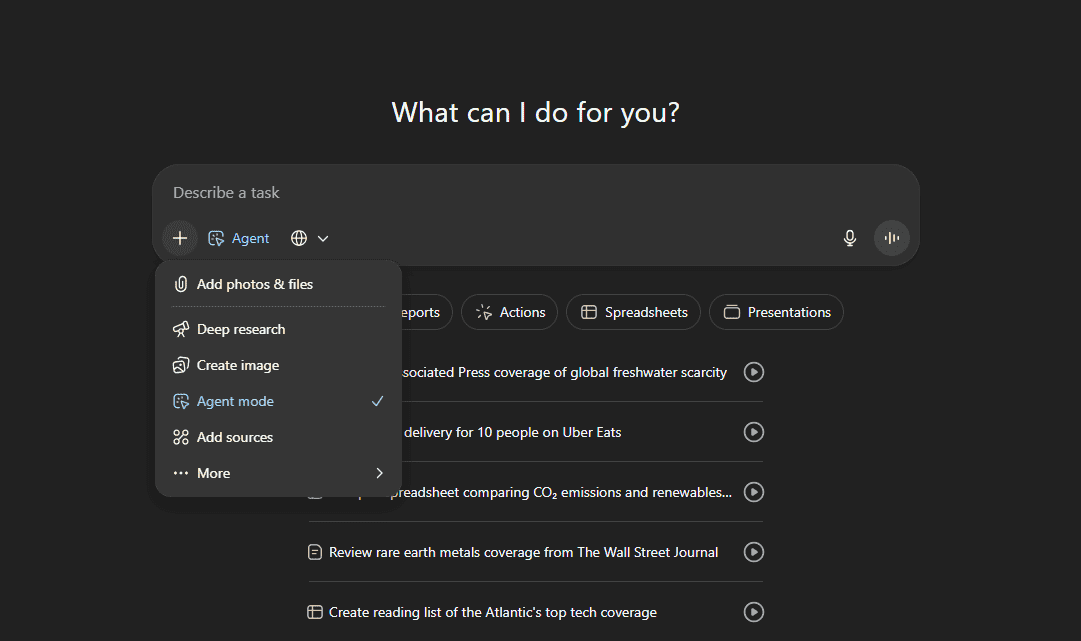
\includegraphics[width=\linewidth,height=0.62\textheight,keepaspectratio]{chatgpt}
  \end{columns}
\end{frame}


% -------- Slide 3: Research / browser assistants --------
\begin{frame}{2. Research and browser assistants}
  \begin{columns}[T,onlytextwidth]
    \column{0.50\textwidth}
      \textbf{Examples}
      \begin{itemize}\setlength\itemsep{0.25em}
        \item \textbf{Perplexity}: AI search with citations.
        \item \textbf{Elicit}: literature search over OpenAlex / Semantic Scholar.
        \item \textbf{NotebookLM}: ground answers in user-uploaded sources.
        \item \textbf{Deep Research} modes inside major chat apps.
      \end{itemize}
      \vspace{0.2cm}
      \textbf{Use}
      \begin{itemize}\setlength\itemsep{0.25em}
        \item Source discovery, evidence extraction, paper triage, background memos.
      \end{itemize}
    \column{0.46\textwidth}
      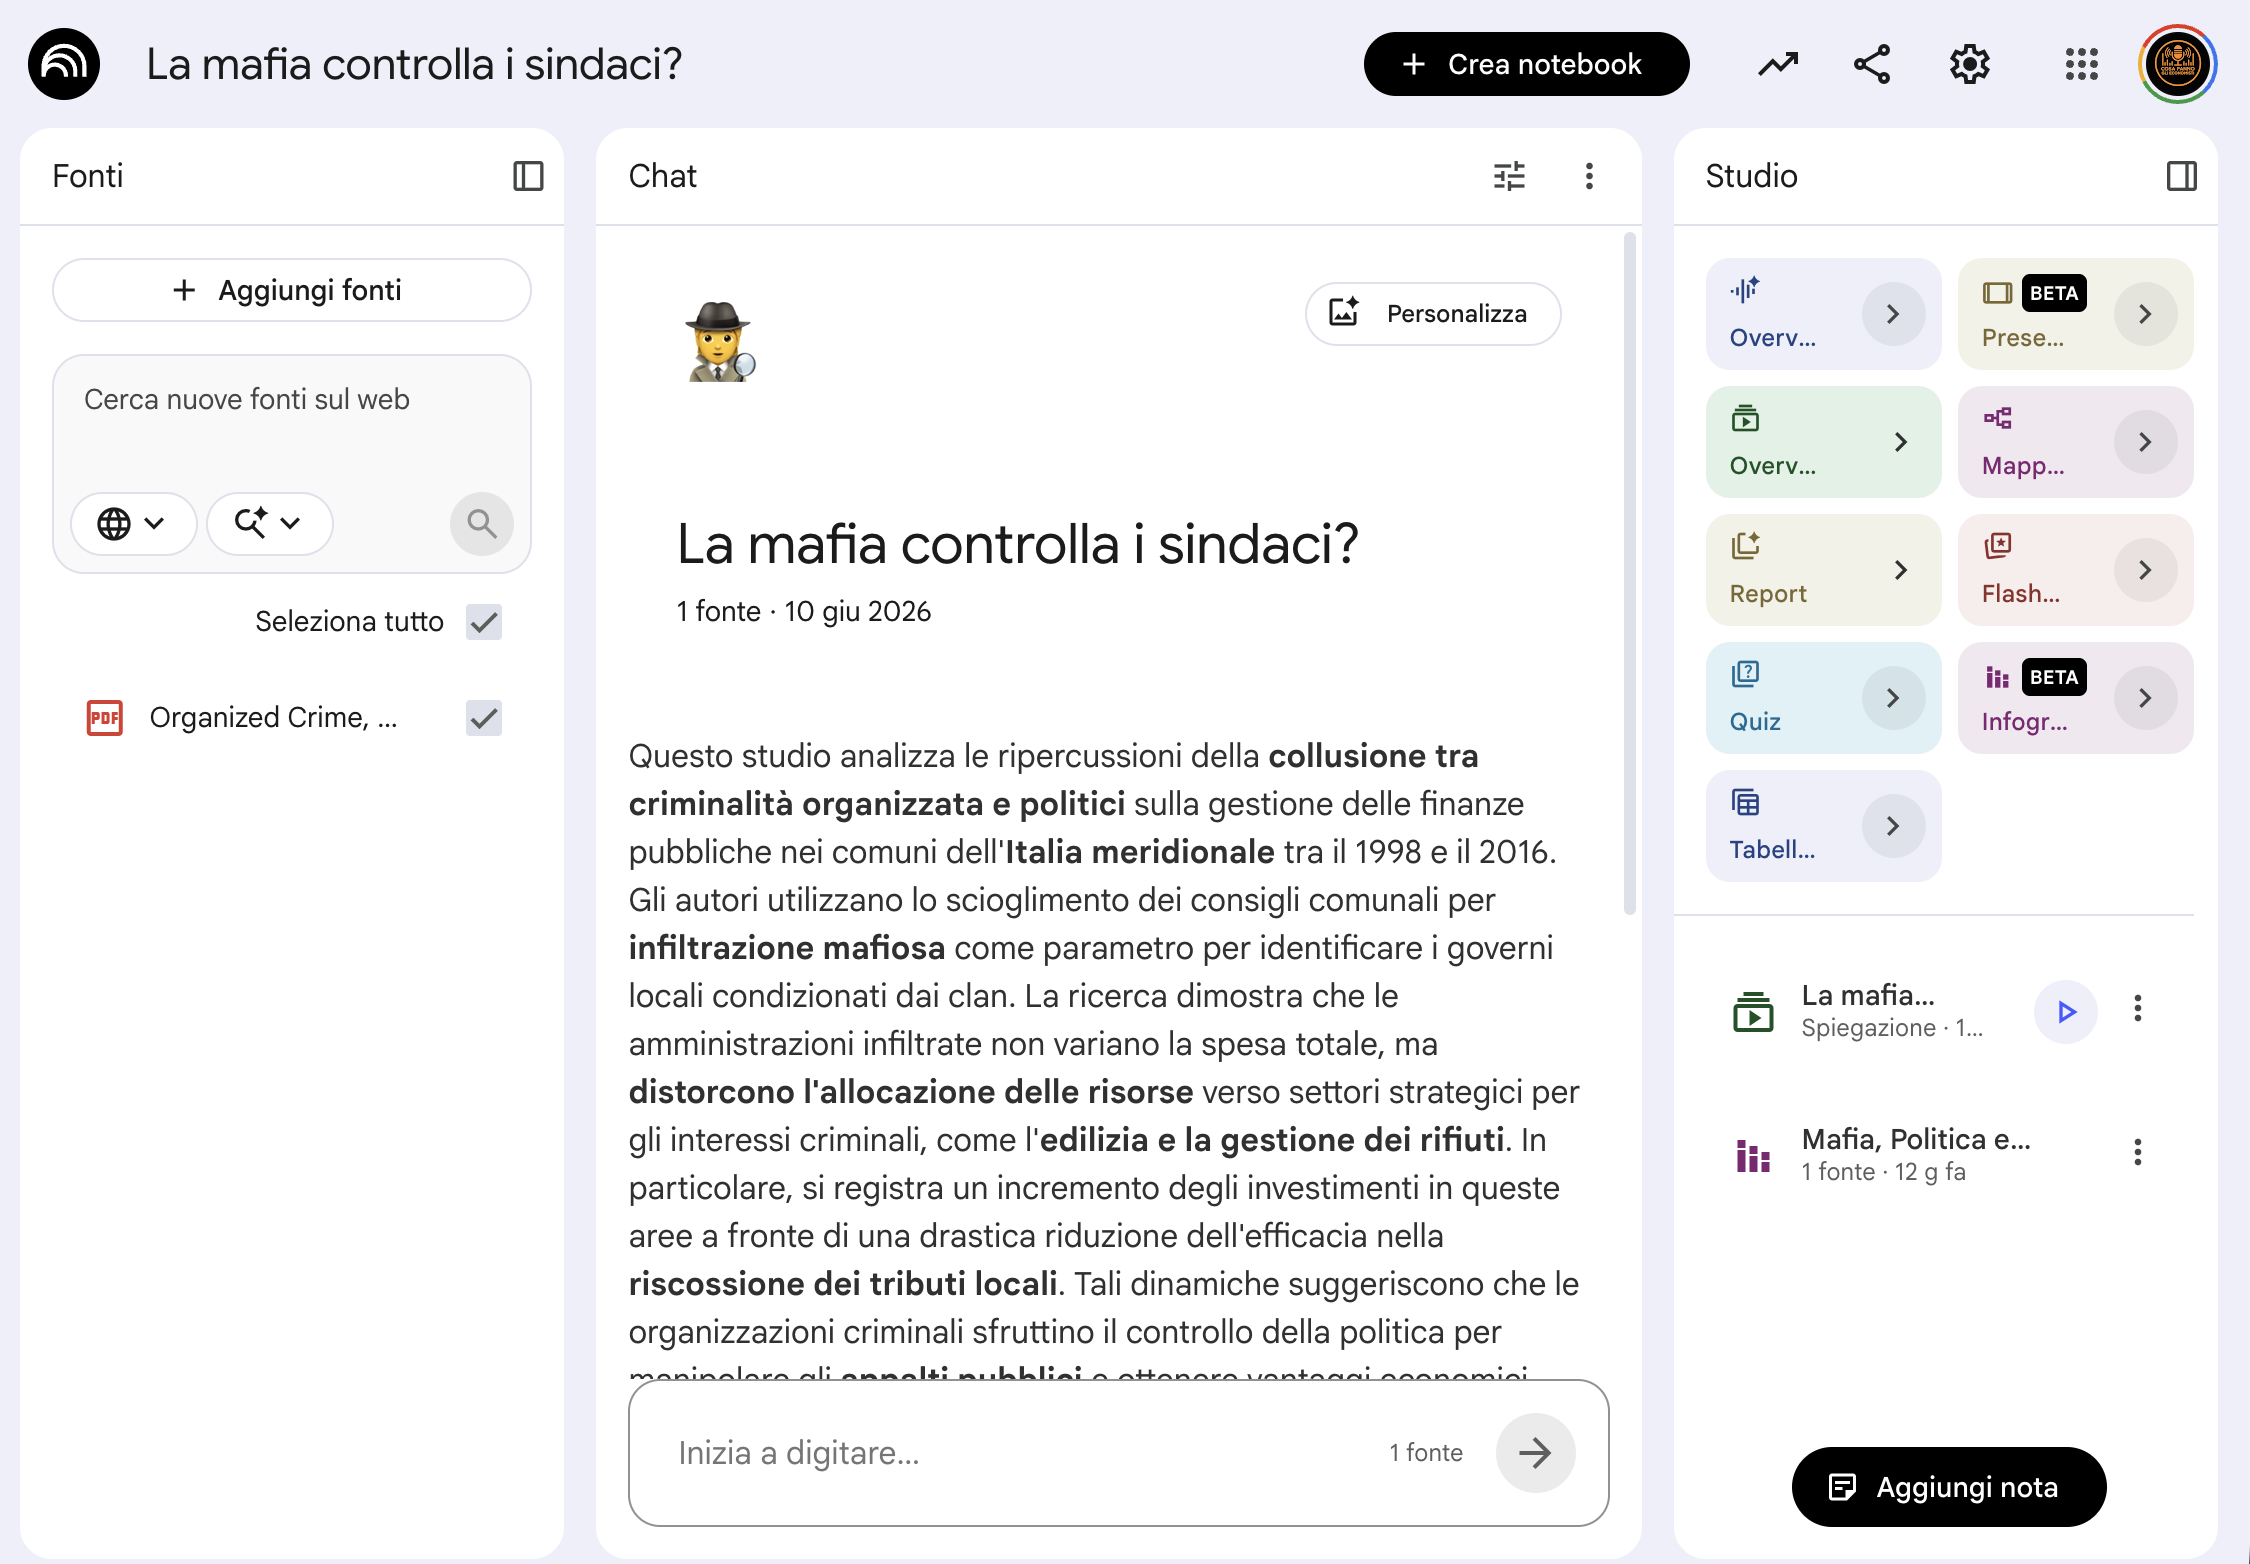
\includegraphics[width=\linewidth,height=0.60\textheight,keepaspectratio]{notebooklm}
  \end{columns}
 
\end{frame}

% -------- Slide 5: IDE agents --------
\begin{frame}{3. IDE agents}
  \begin{columns}[T,onlytextwidth]
    \column{0.48\textwidth}
      \threebullets%
        {Cursor, GitHub Copilot Agent, Antigravity, Codex inside competing IDEs}%
        {Best when the object is a codebase.}%
        {Review happens through diffs, tests and file changes.}
    
      
    \column{0.48\textwidth}
      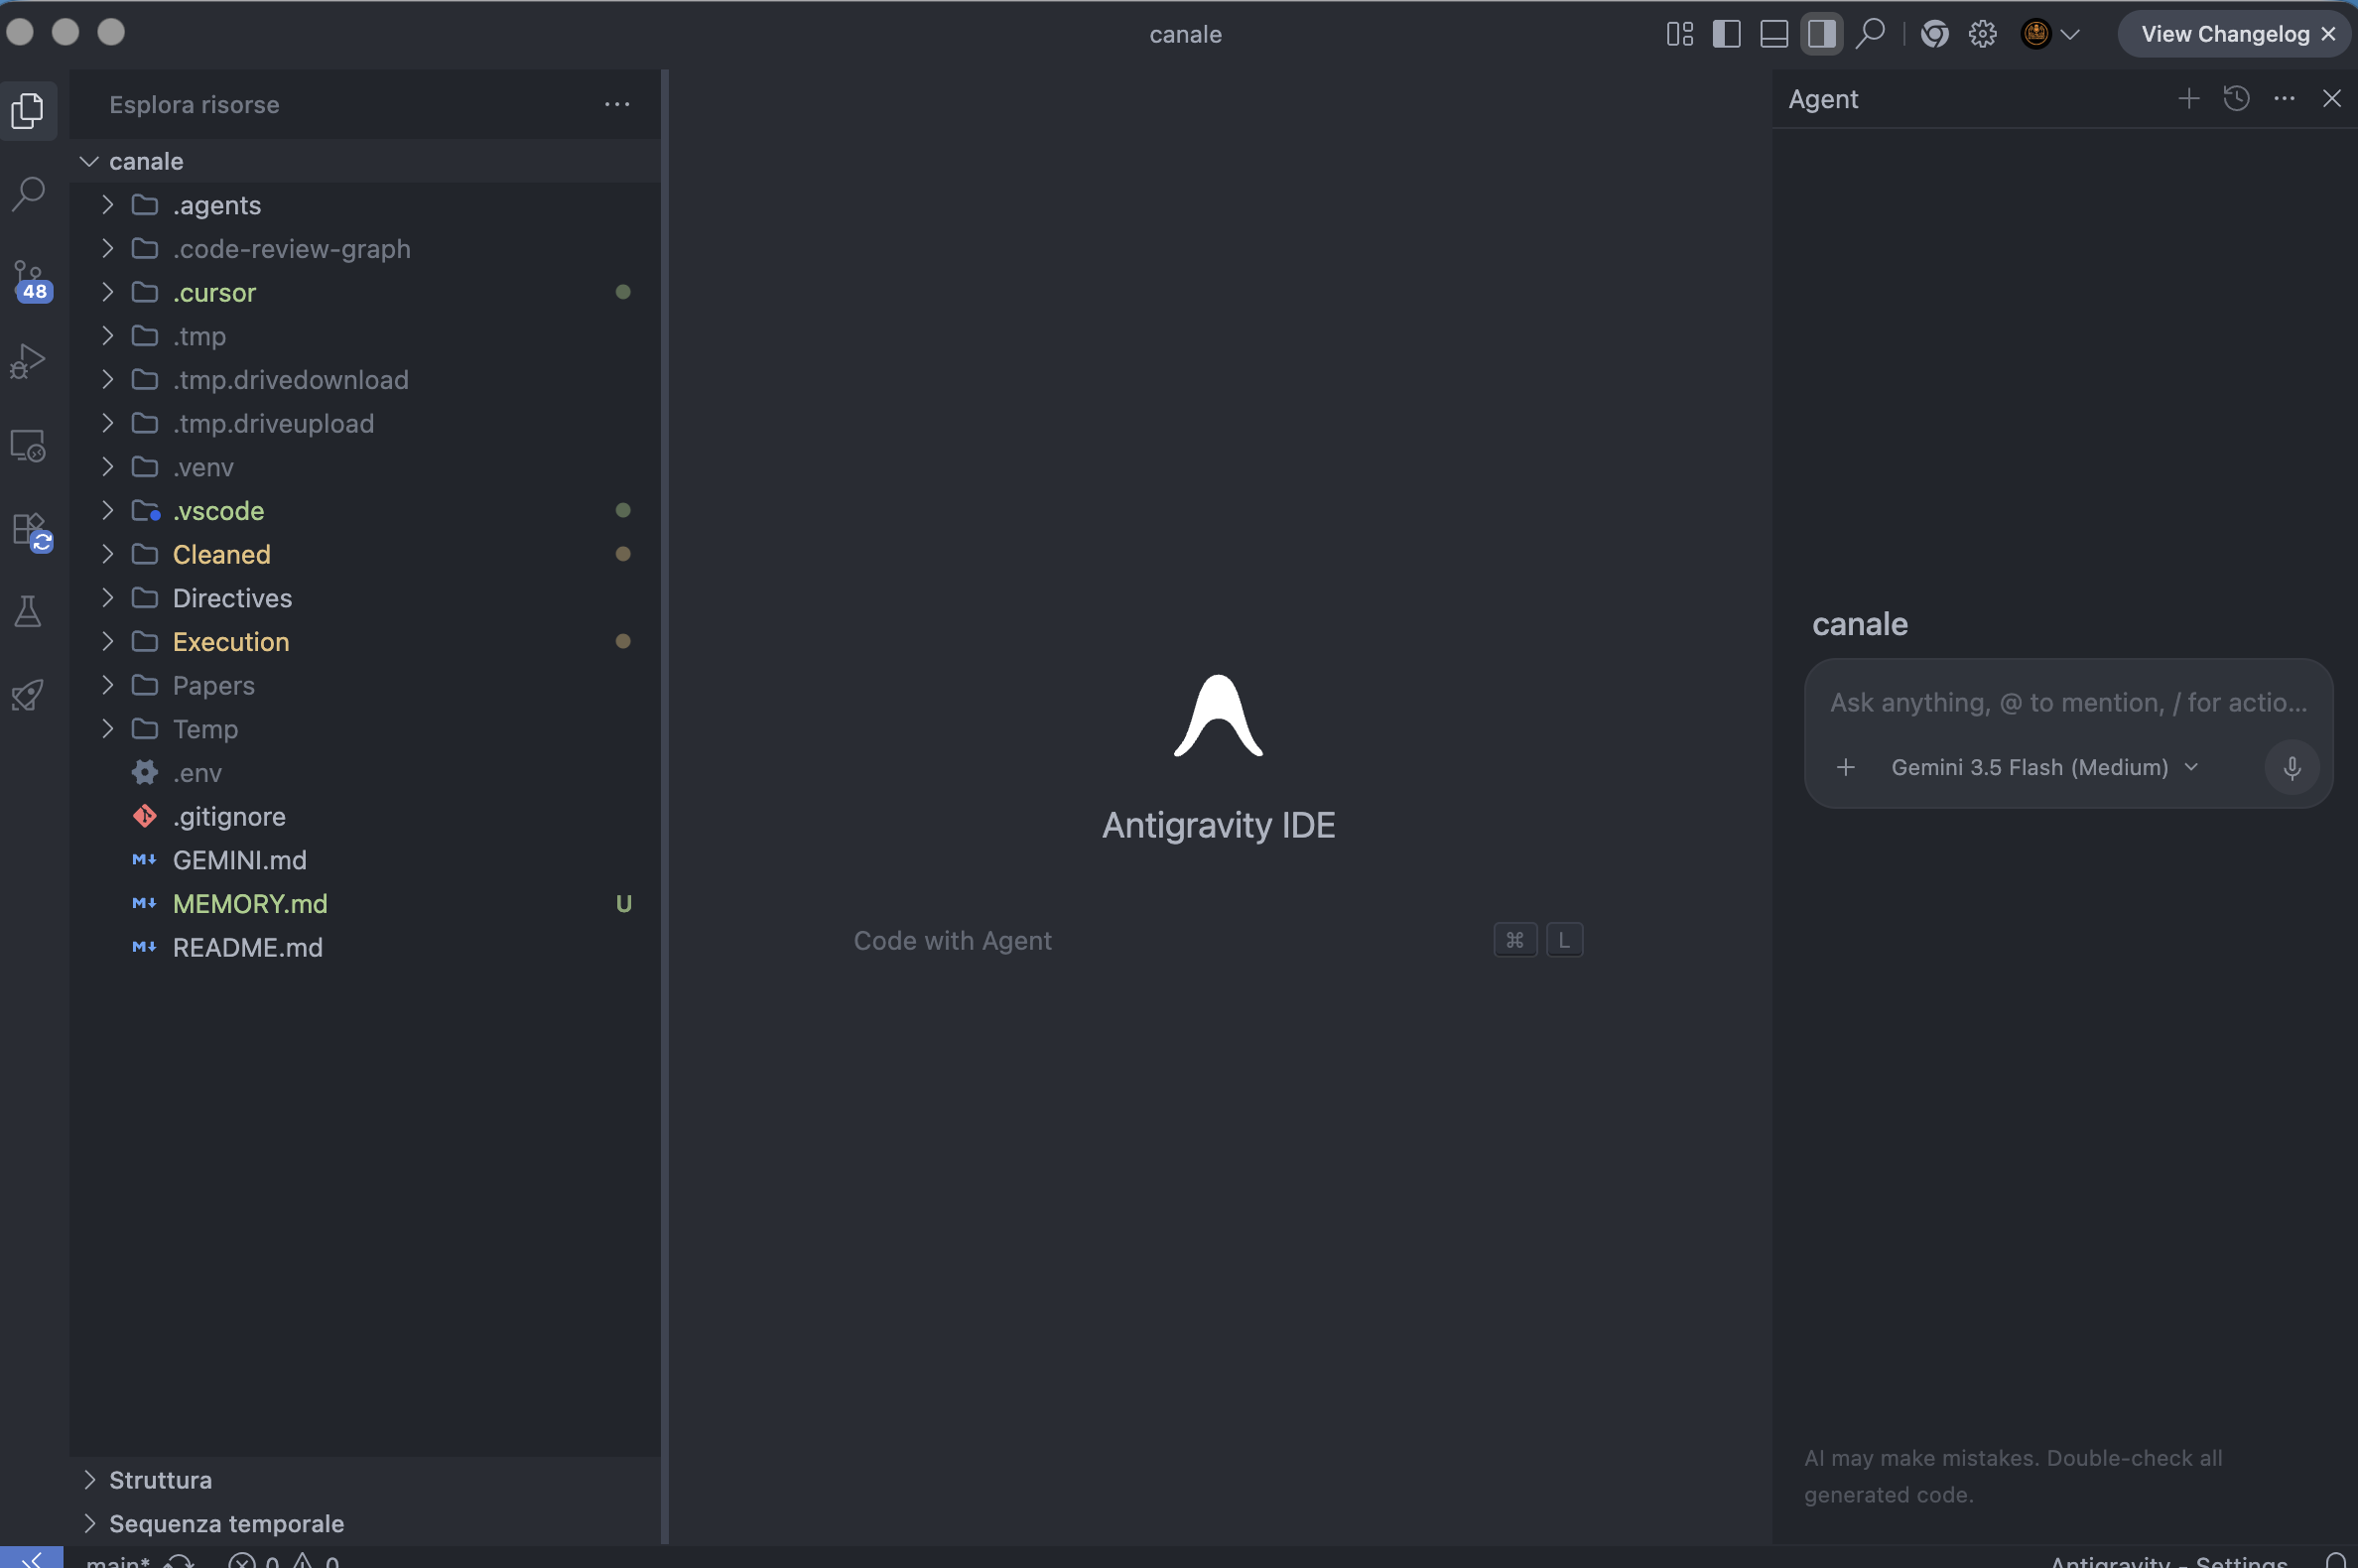
\includegraphics[width=\linewidth,height=0.60\textheight,keepaspectratio]{antigravity_ide}
  \end{columns}
\end{frame}

% -------- Slide 3: Desktop agent apps --------
\begin{frame}{3.1 Desktop agent apps: the IDE boundary is blurring}
  \begin{columns}[T,onlytextwidth]
    \column{0.48\textwidth}
      \textbf{Not only chat in a browser}
      \begin{itemize}\setlength\itemsep{0.3em}
        \item Cursor desktop app, Google Antigravity, Codex app/extension, Claude Code, and similar tools.
        \item They can open folders, inspect files, run commands, edit code, and manage tasks.
        \item The app becomes a control plane around the project, not just a place to ask questions.
      \end{itemize}
    \column{0.48\textwidth}
      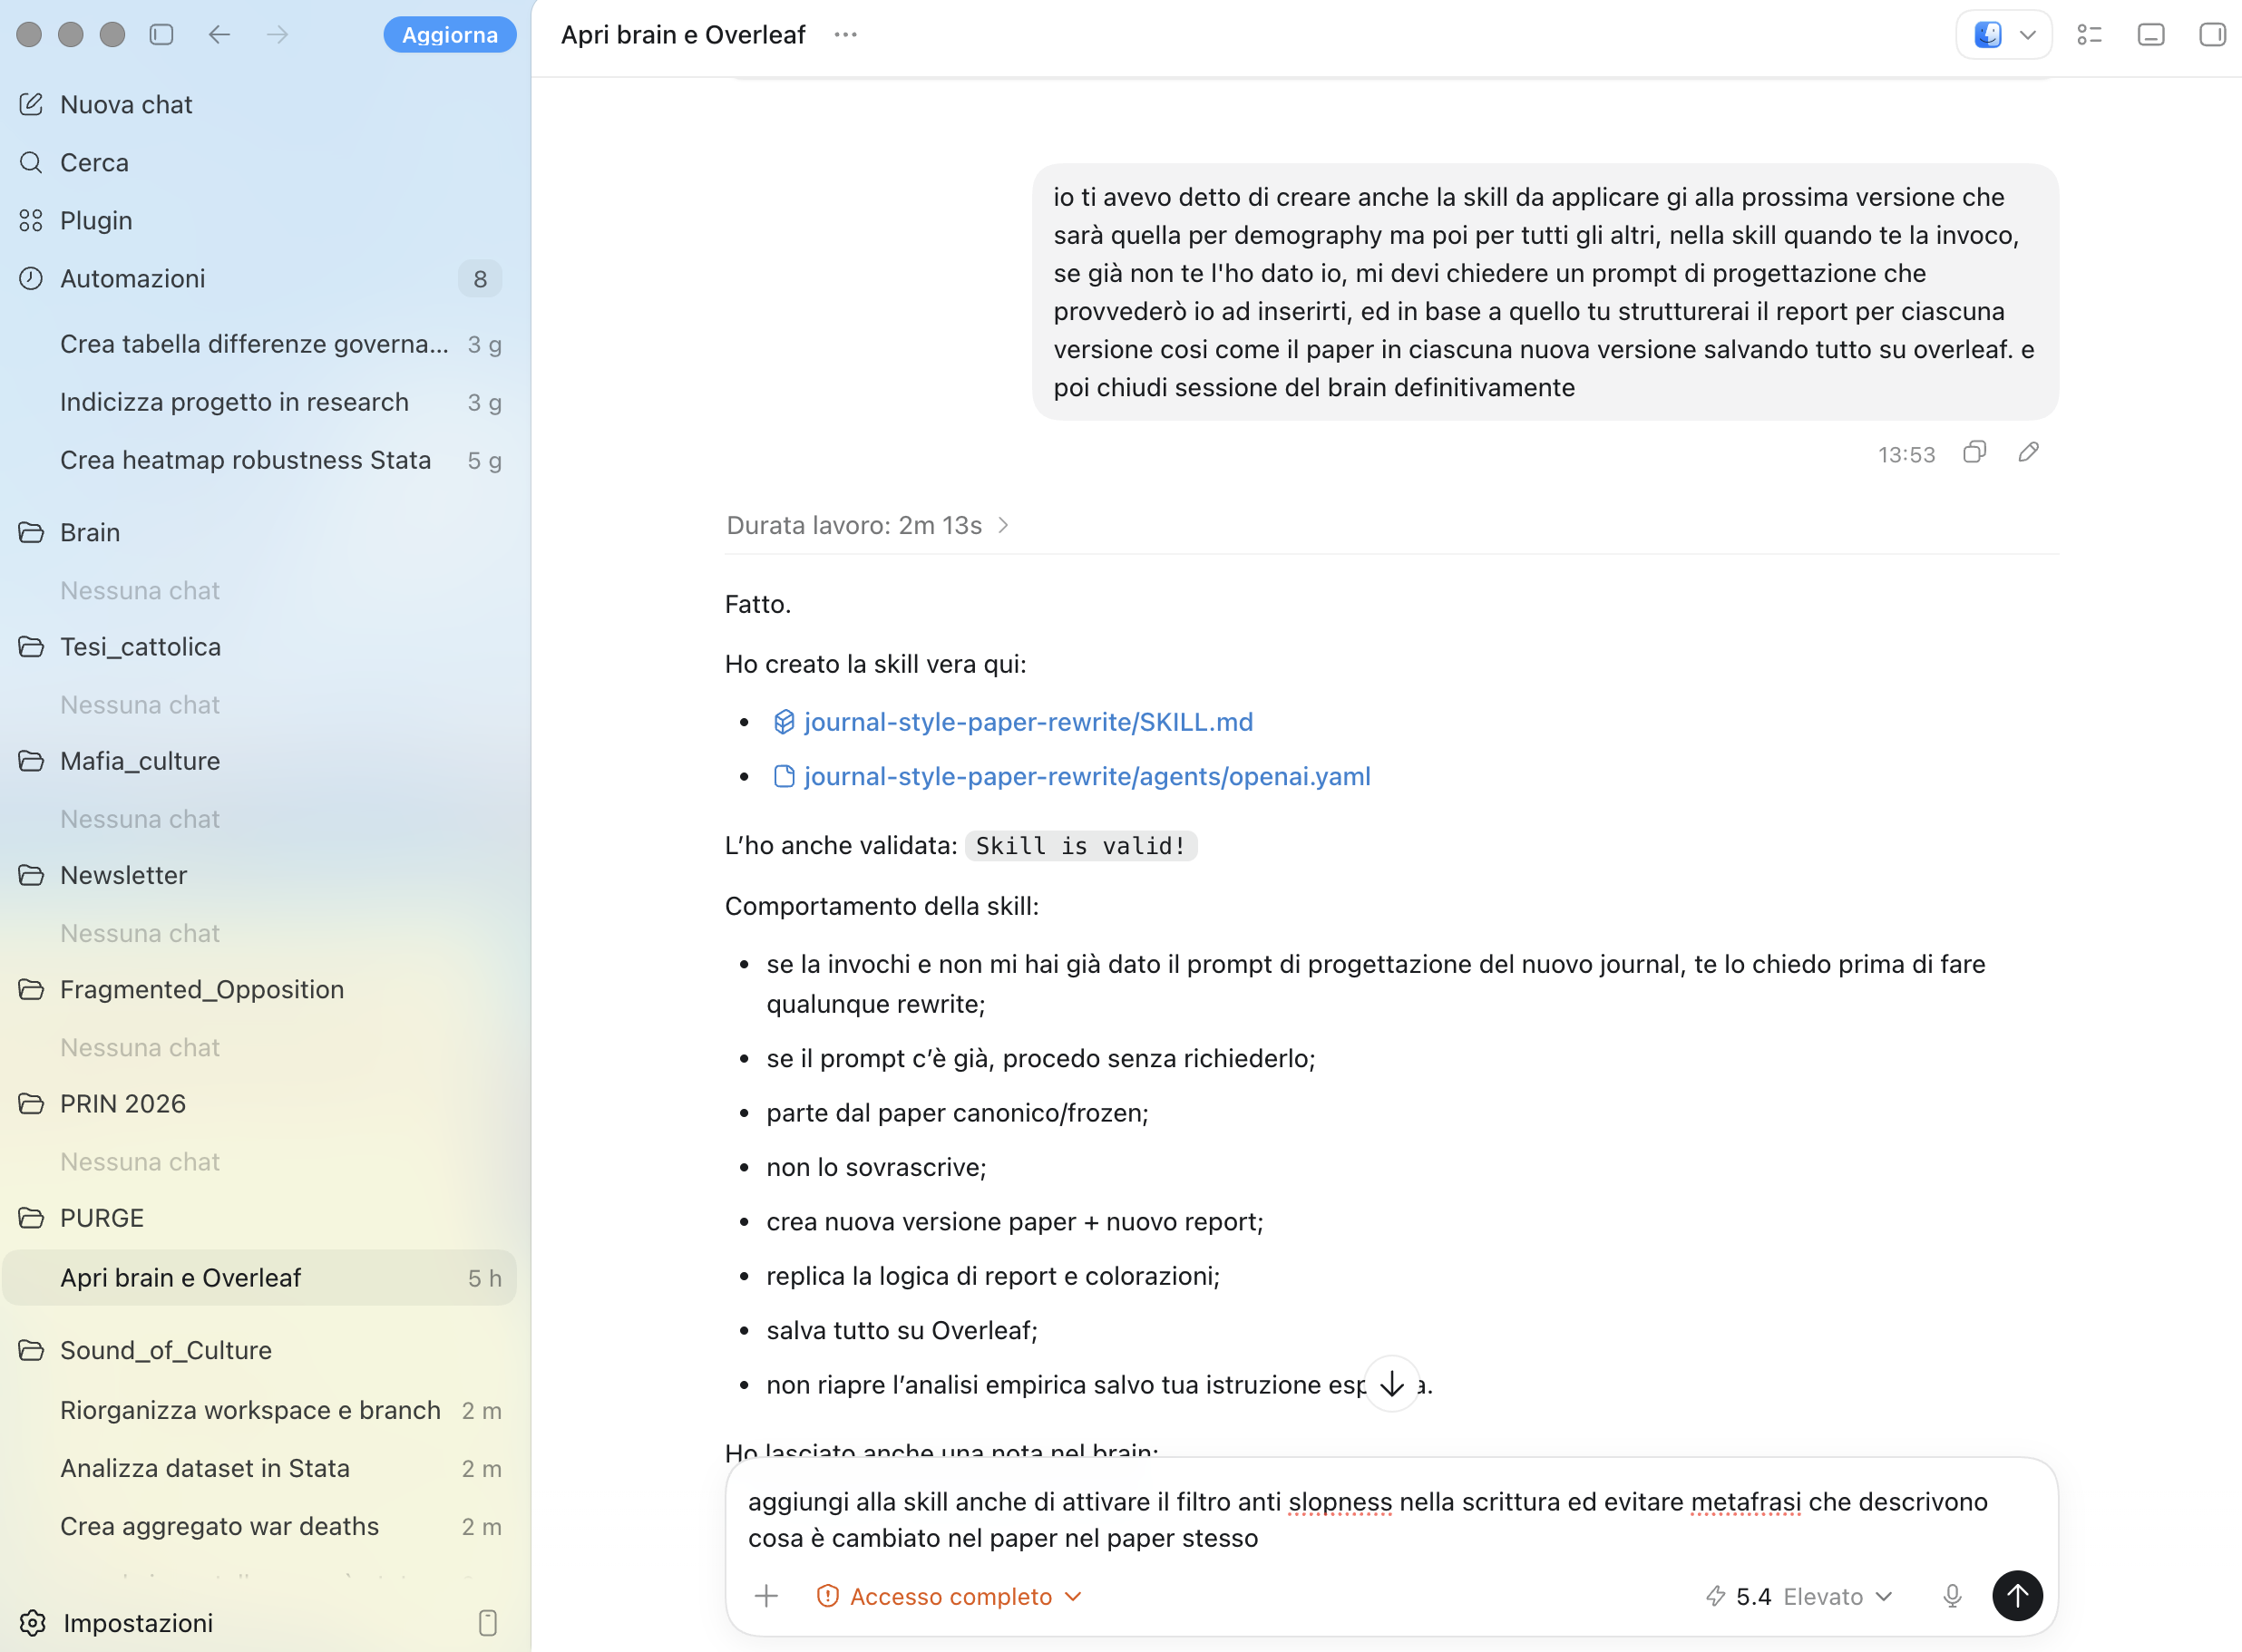
\includegraphics[width=\linewidth,height=0.58\textheight,keepaspectratio]{codex_app}
      \smallsource{Codex desktop app screenshot captured by Marco Le Moglie, 23 June 2026.}
  \end{columns}
  \vspace{0.25cm}
\begin{center}\large\bfseries\color{deepblue}For researchers, the relevant question is: \emph{can I review what changed?}\end{center}
\end{frame}


% -------- Slide 6: CLI agents --------
\begin{frame}{4. CLI agents (and local models)}
  \begin{columns}[T,onlytextwidth]
    \column{0.46\textwidth}
      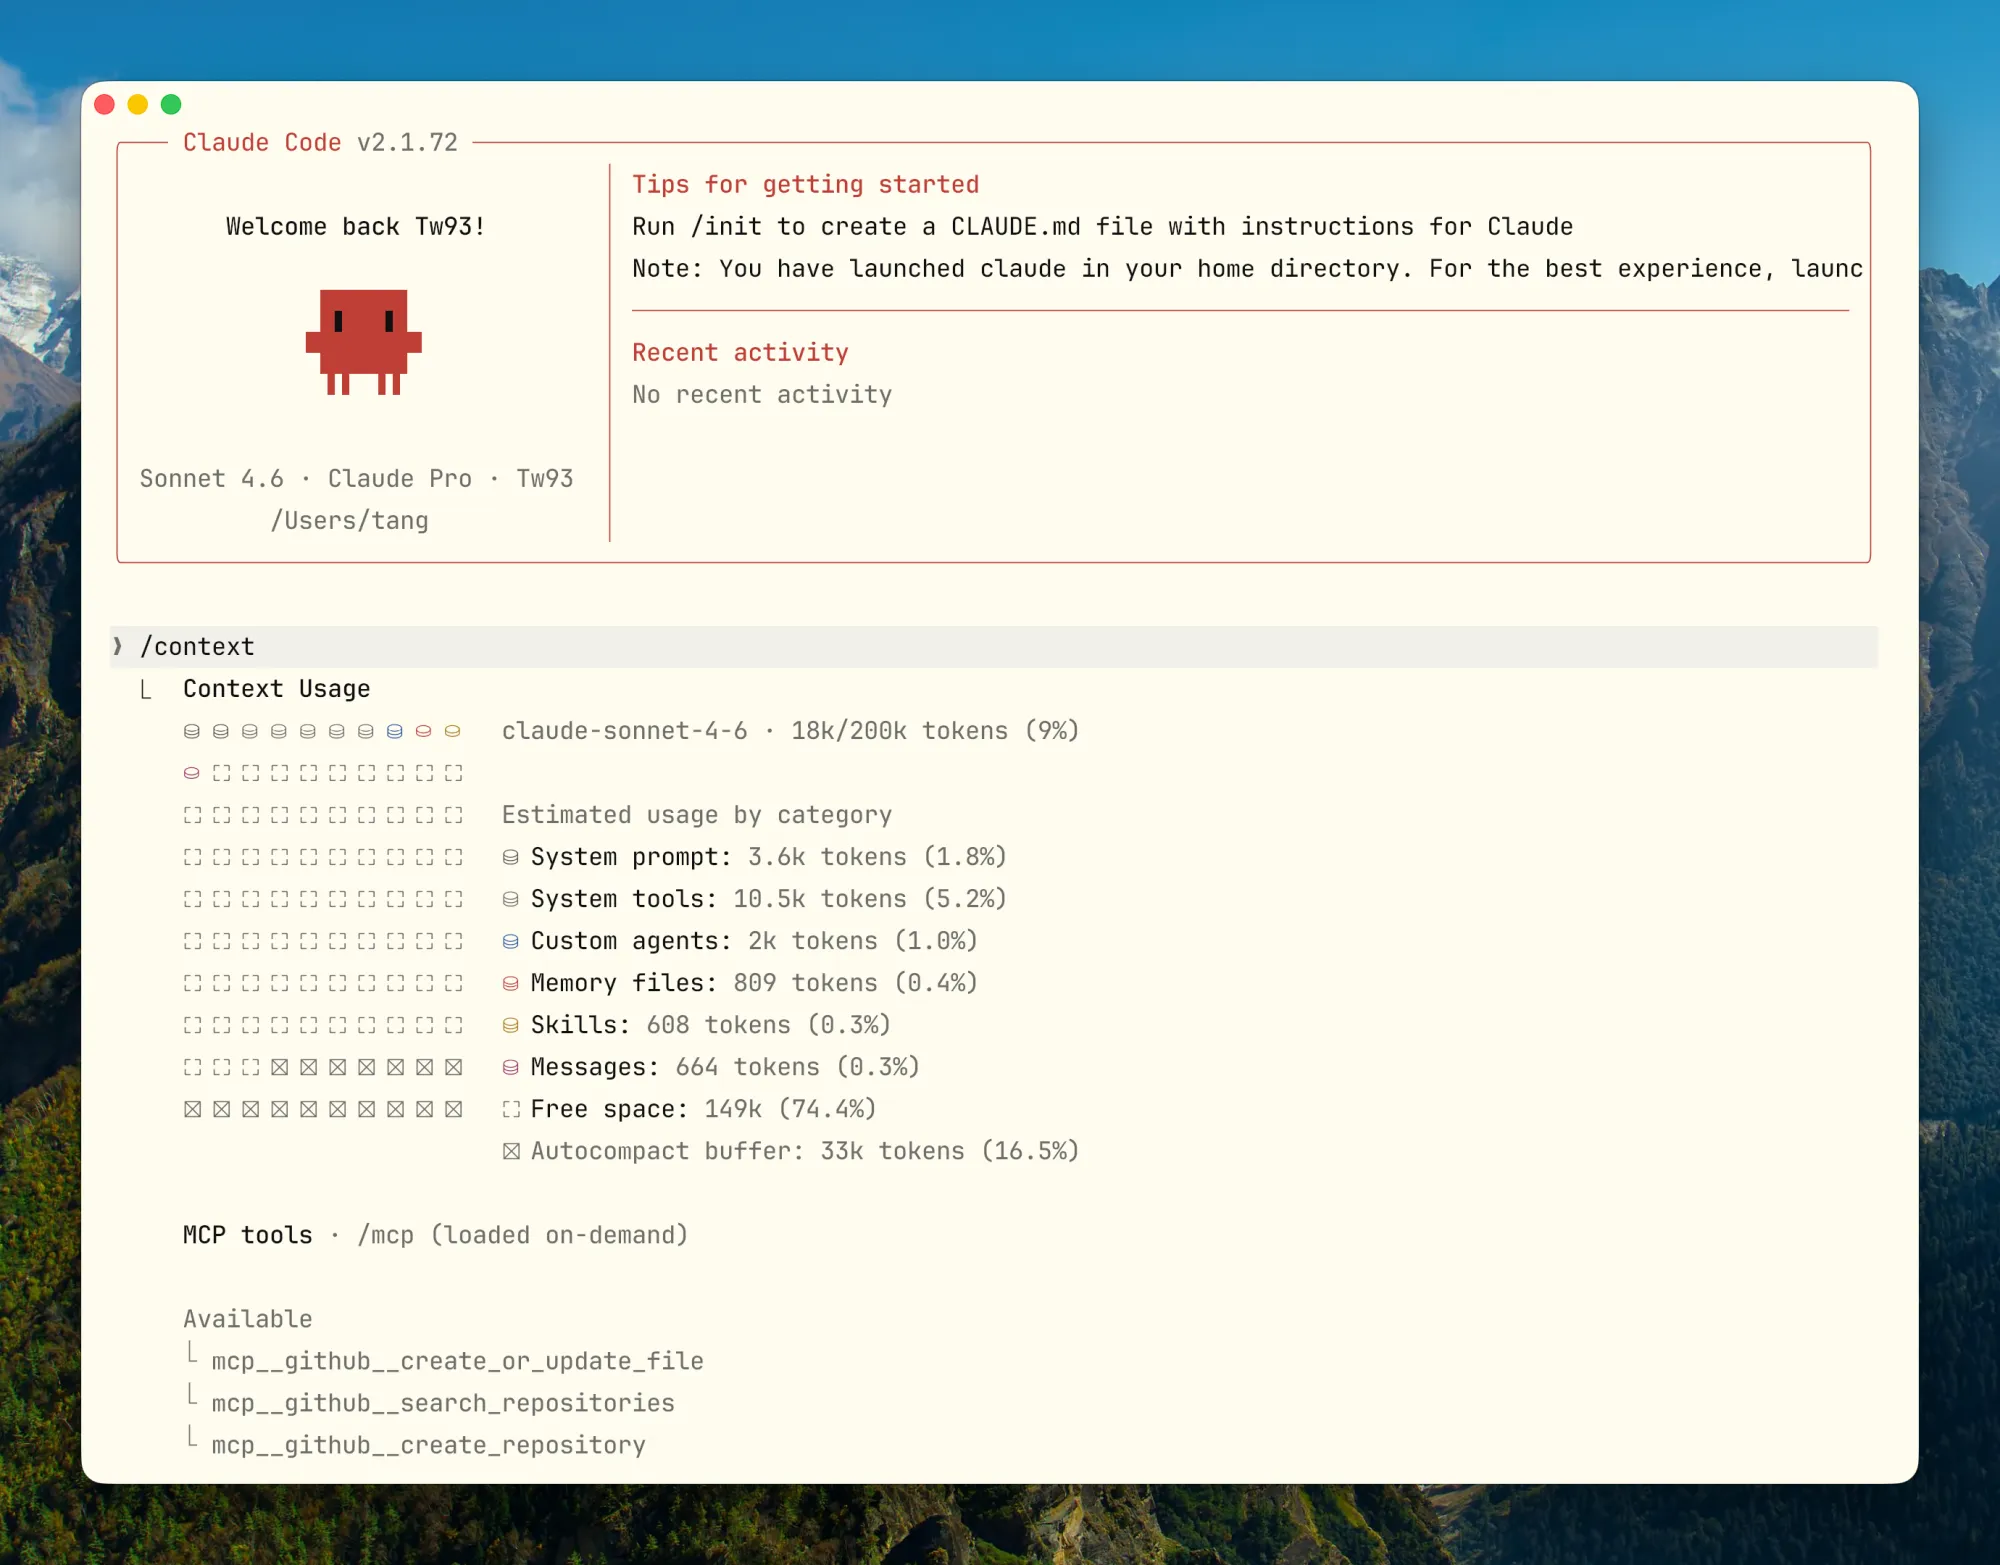
\includegraphics[width=\linewidth,height=0.62\textheight,keepaspectratio]{claude}
    \column{0.50\textwidth}
      \threebullets%
        {Claude Code, OpenAI Codex CLI, Gemini CLI}%
        {They can inspect folders, run commands, edit code, manage processes.}%
        {They consume fewer tokens}
      \vspace{0.2cm}
      \textbf{Local models}
      \begin{itemize}\setlength\itemsep{0.25em}
        \item Ollama, LM Studio, plus open-weight models (Llama, Qwen, Mistral).
        \item Slower and weaker than frontier, but \emph{private}.
      \end{itemize}
  \end{columns}
\end{frame}

% -------- Slide 7: When local vs cloud --------
\begin{frame}{When local is the right answer}
  \begin{columns}[T,onlytextwidth]
    \column{0.48\textwidth}
      \textbf{Local pays off when}
      \begin{itemize}\setlength\itemsep{0.3em}
        \item Data cannot leave the institution.
        \item Tasks are repetitive and the cost would explode in the cloud.
        \item You need full reproducibility and version freezing.
      \end{itemize}
    \column{0.48\textwidth}
      \textbf{Local hurts when}
      \begin{itemize}\setlength\itemsep{0.3em}
        \item Tasks need frontier reasoning.
        \item Hardware is modest (laptop CPU only).
        \item Multi-step agentic workflows: open models still lag.
      \end{itemize}
  \end{columns}
  \vspace{0.5cm}
  \midpoint{For most research, cloud frontier + careful data hygiene wins.}
\end{frame}

% -------- Slide 8: Comparing ecosystems without religion --------
\begin{frame}{Comparing the main ecosystems, without religion}
  \begin{center}
  \begin{tikzpicture}[every node/.style={align=left,font=\small}]
    \node[draw=deepblue,fill=softblue,rounded corners,very thick,
          minimum width=5.8cm,minimum height=2.4cm,text width=5.4cm,inner sep=0.25cm]
          (openai) at (0,1.7) {\textbf{OpenAI}\\Generalist chat + Agent + Codex app/CLI\\\scriptsize \color{muted}watch: cost, limits, plan churn};
    \node[draw=accent,fill=softorange,rounded corners,very thick,
          minimum width=5.8cm,minimum height=2.4cm,text width=5.4cm,inner sep=0.25cm]
          (anthropic) at (6.4,1.7) {\textbf{Anthropic}\\Careful code (Claude Code), strong defaults\\\scriptsize \color{muted}watch: usage caps, restricted regions};
    \node[draw=deepblue,fill=softgreen,rounded corners,very thick,
          minimum width=5.8cm,minimum height=2.4cm,text width=5.4cm,inner sep=0.25cm]
          (google) at (0,-1.5) {\textbf{Google}\\Long context + Search + Antigravity + Gemini CLI\\\scriptsize \color{muted}watch: product churn, naming};
    \node[draw=accent,fill=softpurple,rounded corners,very thick,
          minimum width=5.8cm,minimum height=2.4cm,text width=5.4cm,inner sep=0.25cm]
          (cursor) at (6.4,-1.5) {\textbf{Cursor}\\IDE-native, multi-model, agent-first\\\scriptsize \color{muted}watch: subscription / usage split};
  \end{tikzpicture}
  \end{center}
  \vspace{0.1cm}
  \begin{center}\scriptsize\color{muted}Also: Grok / xAI; Perplexity / Elicit / NotebookLM for search; Llama / Qwen / Mistral for local.\end{center}
\end{frame}

% -------- Slide 9: Choose by task, not by brand --------
\begin{frame}{Choose by task, not by brand}
  \vspace{0.2cm}
  \begin{center}
  \begin{tabularx}{0.92\linewidth}{>{\bfseries\color{deepblue}}lX}
  \toprule
  Thinking, writing, light analysis & Chat app (any frontier).\\
  Source discovery, evidence triage & Research assistant + chat for synthesis.\\
  Coding, replication packages, table generation & IDE agent or desktop agent app.\\
  Batch jobs, scripted pipelines, server work & CLI agent.\\
  Sensitive data, full reproducibility & Local model where feasible; otherwise enterprise plan with no training.\\
  \bottomrule
  \end{tabularx}
  \end{center}
  \vspace{0.5cm}
  \midpoint{Most real workflows combine two or three of the solutions above.}
\end{frame}

% =============================================================
% Block 4 -- Cost, privacy, governance (7 slides)
% =============================================================

\sectionframe[accent]{Part 4 -- Cost, privacy, governance}

% -------- Slide 1: Subscription vs API --------
\begin{frame}{Subscription vs API}
  \begin{columns}[T,onlytextwidth]
    \column{0.48\textwidth}
      \textbf{Subscription (consumer / Pro / Team)}
      \begin{itemize}\setlength\itemsep{0.3em}
        \item Flat monthly price.
        \item Limits are often soft, dynamic, hard to compare.
        \item ``Unlimited'' is rarely uncontrolled: throttling, queueing, capability gating.
      \end{itemize}
    \column{0.48\textwidth}
      \textbf{API / metered usage}
      \begin{itemize}\setlength\itemsep{0.3em}
        \item Cost is measurable per token or call.
        \item Easier to budget, easier to overspend.
        \item Required for IDE/CLI agents that call many tools.
      \end{itemize}
  \end{columns}
  \vspace{0.5cm}
  \begin{center}\Large\color{accent}\bfseries For agents, ``unlimited'' rarely means uncontrolled.\end{center}
 
\end{frame}

% -------- Slide 2: Pricing logic chart --------
\begin{frame}{The four levers that drive your bill}
  \begin{columns}[T,onlytextwidth]
    \column{0.48\textwidth}
      \begin{tikzpicture}[every node/.style={align=center,font=\small}]
        \node[draw=deepblue,fill=softblue,rounded corners,very thick,
              minimum width=4.8cm,minimum height=0.72cm,text width=4.5cm]
              (ctx){\textbf{Context size}\\\scriptsize files, history, tool outputs};
        \node[draw=accent,fill=softorange,rounded corners,very thick,
              minimum width=4.8cm,minimum height=0.72cm,text width=4.5cm,
              below=0.32cm of ctx]
              (calls){\textbf{Tool calls}\\\scriptsize each call adds prompts and results};
        \node[draw=deepblue,fill=softgreen,rounded corners,very thick,
              minimum width=4.8cm,minimum height=0.72cm,text width=4.5cm,
              below=0.32cm of calls]
              (ret){\textbf{Retries}\\\scriptsize errors, self-checks, sub-agents};
        \node[draw=accent,fill=softpurple,rounded corners,very thick,
              minimum width=4.8cm,minimum height=0.72cm,text width=4.5cm,
              below=0.32cm of ret]
              (mod){\textbf{Model tier}\\\scriptsize price per million tokens};
        \node[draw=dark,fill=white,line width=1pt,rounded corners,
              minimum width=4.8cm,minimum height=0.8cm,text width=4.5cm,
              below=0.45cm of mod]
              (cost){\textbf{\color{deepblue}Total cost per task}};
        \draw[->,thick,color=muted] (ctx) -- (calls);
        \draw[->,thick,color=muted] (calls) -- (ret);
        \draw[->,thick,color=muted] (ret) -- (mod);
        \draw[->,thick,color=muted] (mod) -- (cost);
      \end{tikzpicture}
    \column{0.48\textwidth}
      \fourbullets%
        {\textbf{Context} grows with files, browsing, history.}%
        {\textbf{Tool calls} multiply with autonomy.}%
        {\textbf{Retries} are silent: errors, validation, sub-agents.}%
        {\textbf{Model tier} can differ 10$\times$--50$\times$ in price per token.}
      \vspace{0.3cm}
      \begin{center}\small\color{accent}\bfseries A chat session ignores three of these. An agent uses all four.\end{center}
  \end{columns}
\end{frame}

% -------- Slide 3: Cost spike case --------
\begin{frame}{What a real cost spike looks like}
  \vspace{0.2cm}
  \begin{center}
  \begin{tabularx}{0.94\linewidth}{>{\bfseries\color{deepblue}}lXl}
  \toprule
  Workload & Description & Tokens (approx.)\\
  \midrule
  Chat question & ``Explain heteroskedasticity in two lines.'' & $\sim 0.5$k\\
  Long reading & ``Summarise this 30-page PDF.'' & $\sim 25$k\\
  IDE one-shot edit & ``Fix this regression call.'' & $\sim 8$k\\
  IDE agent task & ``Re-run all tables and verify.'' & $\sim 80$--$200$k\\
  Multi-agent research run & ``Replicate Section 4 end-to-end.'' & $\sim 500$k--$2$M\\
  \bottomrule
  \end{tabularx}
  \end{center}
  \vspace{0.4cm}
  \midpoint{Same UI. Two orders of magnitude difference in cost.}
  
\end{frame}

% -------- Slide 4: Does it train on my data? --------
\begin{frame}{Does it train on my data?}
  \begin{columns}[T,onlytextwidth]
    \column{0.50\textwidth}
      \textbf{The honest answer:}\\[0.2cm]
      It depends on the \emph{provider}, \emph{plan}, \emph{workspace} and \emph{settings}.
      \vspace{0.4cm}
      \begin{itemize}\setlength\itemsep{0.3em}
        \item Consumer plans: often \textbf{default to training} unless you opt out.
        \item Business/Enterprise plans: usually \textbf{do not train} on your data by default.
        \item API: usually no training, but check retention policy.
      \end{itemize}
    \column{0.46\textwidth}
      \textbf{What to verify}
      \begin{itemize}\setlength\itemsep{0.3em}
        \item Account type (personal vs business).
        \item Workspace data-use settings.
        \item Region and applicable law (GDPR, US sectoral).
        \item Tool-specific data flow (browsers, retrieval, sub-agents).
      \end{itemize}
      \vspace{0.2cm}
      \begin{center}\small\color{accent}\bfseries Settings change. Verify, do not assume.\end{center}
  \end{columns}
  \smallsource{See provider documentation: \citet{openai_pricing,anthropic_pricing,google_ai_plans,cursor_pricing}.}
\end{frame}

% -------- Slide 5: Data risk in economics research --------
\begin{frame}{Data risk in economics research}
  \vspace{0.2cm}
  \begin{center}
  \begin{tabularx}{0.92\linewidth}{>{\bfseries\color{deepblue}}lX}
  \toprule
  High risk & Microdata, administrative data, embargoed data, confidential referee reports, unpublished IRB-restricted material.\\
  Medium risk & Unpublished drafts, grant ideas, coauthors' working notes, identifiable interview transcripts.\\
  Lower risk & Public documentation, synthetic examples, teaching material, published papers.\\
  \bottomrule
  \end{tabularx}
  \end{center}
  \vspace{0.4cm}
  \begin{center}\Large\color{accent}\bfseries When in doubt: anonymise, abstract, or use a sandbox.\end{center}
  
\end{frame}

% -------- Slide 6: Institutional and IRB considerations --------
\begin{frame}{Institutional and IRB considerations}
  \begin{columns}[T,onlytextwidth]
    \column{0.48\textwidth}
      \textbf{Things to clarify with your institution}
      \begin{itemize}\setlength\itemsep{0.3em}
        \item Approved vendors and data-processing agreements.
        \item Whether AI processing of human-subjects data is covered by existing IRB protocols.
        \item Storage, retention, and right-to-erasure obligations.
      \end{itemize}
    \column{0.48\textwidth}
      \textbf{Things to clarify in journals}
      \begin{itemize}\setlength\itemsep{0.3em}
        \item Disclosure requirements for AI use.
        \item Reproducibility expectations: AEA Data Editor and similar.
        \item Authorship: an agent is not an author.
      \end{itemize}
  \end{columns}
  \vspace{0.5cm}
  \midpoint{The rules are still moving. Document what you did.}
  \smallsource{See Vilhuber \citeyearpar{vilhuber_hdsr_2020} on reproducibility norms; consult AEA Data Editor guidance for the latest disclosure standards.}
\end{frame}

% -------- Slide 7: Practical safeguards --------
\begin{frame}{Practical safeguards that actually work}
  \begin{columns}[T,onlytextwidth]
    \column{0.48\textwidth}
      \textbf{Budget and pace}
      \begin{itemize}\setlength\itemsep{0.3em}
        \item Set an explicit monthly budget per project.
        \item Ask the agent for a plan \emph{before} execution.
        \item Use a cheaper model for scanning, frontier for the hard step.
      \end{itemize}
    \column{0.48\textwidth}
      \textbf{Containment}
      \begin{itemize}\setlength\itemsep{0.3em}
        \item Sandbox: run agents inside a constrained folder/VM.
        \item Read-only mode for first passes.
        \item Kill switch: easy to interrupt; nothing irreversible without confirmation.
      \end{itemize}
  \end{columns}
  \vspace{0.4cm}
  \midpoint{Safety is mostly process design, not magic settings.}
\end{frame}

% =============================================================
% Block 5 -- Reliability and control (5 slides)
% =============================================================

\sectionframe{Part 5 -- Reliability and control}

% -------- Slide 1: Hallucinations are not only fake citations --------
\begin{frame}{Hallucinations are not only fake citations}
  \vspace{0.2cm}
  \begin{center}
  \begin{tabularx}{0.92\linewidth}{>{\bfseries\color{deepblue}}lX}
  \toprule
  Citation hallucination & A plausible but nonexistent paper, dataset, or table.\\
  Code hallucination & A function that runs, but implements the wrong logic.\\
  Statistical hallucination & Correct syntax, wrong interpretation (e.g., wrong fixed effects).\\
  Workflow hallucination & Task marked complete without real verification (no test, no log, no diff).\\
  \bottomrule
  \end{tabularx}
  \end{center}
  \vspace{0.4cm}
  \midpoint{In agents, the most dangerous hallucination is ``done''.}
  \smallsource{Hallucination taxonomy adapted from Ji et al.\ \citeyearpar{ji_acm_2023}.}
\end{frame}

% -------- Slide 2: Automation bias and overtrust --------
\begin{frame}{Automation bias and overtrust}
  \begin{columns}[T,onlytextwidth]
    \column{0.48\textwidth}
      \threebullets%
        {Humans systematically over-trust automated outputs \citep{skitka_1999_automation_bias}.}%
        {The smoother and more confident the output, the stronger the bias.}%
        {AI outputs are smoother and more confident than human drafts.}
    \column{0.48\textwidth}
      \textbf{What this looks like in practice}
      \begin{itemize}\setlength\itemsep{0.3em}
        \item Accepting a regression specification ``because the output table looks reasonable''.
        \item Copy-pasting a literature summary without reading the cited papers.
        \item Skipping unit tests because the agent ``already checked''.
      \end{itemize}
  \end{columns}
  \vspace{0.4cm}
  \midpoint{Polished prose is not validated reasoning.}
\end{frame}

% -------- Slide 3: Verification by design --------
\begin{frame}{Verification by design}
  \begin{center}
  \begin{tikzpicture}[every node/.style={align=center,font=\small}]
    \node[draw=deepblue,fill=softblue,rounded corners,very thick,
          minimum width=3.2cm,minimum height=1.1cm,text width=3cm]
          (test){\textbf{Tests}\\\scriptsize unit, smoke, golden};
    \node[draw=accent,fill=softorange,rounded corners,very thick,
          minimum width=3.2cm,minimum height=1.1cm,text width=3cm,right=0.7cm of test]
          (diff){\textbf{Diffs}\\\scriptsize visible, reviewable};
    \node[draw=deepblue,fill=softgreen,rounded corners,very thick,
          minimum width=3.2cm,minimum height=1.1cm,text width=3cm,right=0.7cm of diff]
          (logs){\textbf{Logs}\\\scriptsize commands, outputs};
    \node[draw=accent,fill=softpurple,rounded corners,very thick,
          minimum width=3.2cm,minimum height=1.1cm,text width=3cm,right=0.7cm of logs]
          (rev){\textbf{Review}\\\scriptsize human or second agent};
    \draw[->,thick,color=muted] (test)--(diff);
    \draw[->,thick,color=muted] (diff)--(logs);
    \draw[->,thick,color=muted] (logs)--(rev);
  \end{tikzpicture}
  \end{center}
  \vspace{0.4cm}
  \begin{center}\large\color{deepblue}\bfseries Verification cannot be an afterthought; it must be a slot in the workflow.\end{center}
  \vspace{0.2cm}
  \begin{center}\small\color{muted}For research code: at least one test per table, every change as a commit, every command in a log.\end{center}
\end{frame}

% -------- Slide 4: When NOT to use an agent --------
\begin{frame}{When \emph{not} to use an agent}
  \vspace{0.2cm}
  \begin{center}
  \begin{tabularx}{0.92\linewidth}{>{\bfseries\color{deepblue}}lX}
  \toprule
  Identification & The hardest, most causal-inference-specific step.\\
  Confidential data & Where the privacy boundary is unclear.\\
  Final claims & The exact wording of theorems, abstracts, conclusions.\\
  Trust-critical artefacts & Replication packages submitted to a data editor.\\
  Disagreements with coauthors & Resolve by talking, not by prompting.\\
  \bottomrule
  \end{tabularx}
  \end{center}
  \vspace{0.4cm}
  \begin{center}\Large\color{accent}\bfseries Delegating these does not save time; it transfers risk.\end{center}
\end{frame}

% -------- Slide 5: The local alignment problem --------
\begin{frame}{The local alignment problem}
  \begin{center}\Large\bfseries\color{deepblue}The agent optimises for completing the task.\\You care about doing good research.\end{center}
  \vspace{0.4cm}
  \threebullets%
    {Plausible code is not valid code.}%
    {A complete table is not a correct table.}%
    {A polished paragraph is not a justified claim.}
  \vspace{0.5cm}
  \midpoint{The alignment gap is not in 2030; it is in your next prompt.}
\end{frame}

% =============================================================
% Block 6 -- Agentic architecture (8 slides)
% Rules / memory stack / Obsidian KB vs RAG / MCP vs API vs CLI /
% subagents / skills-hooks / orchestration / Plan-Implement loop
% =============================================================

\sectionframe[accent]{Part 6 -- Agentic architecture}

% -------- Slide 1: Rules and Markdown files --------
\begin{frame}{Rules and Markdown files: prompts that stay}
  \begin{columns}[T,onlytextwidth]
    \column{0.42\textwidth}
      \bigpoint{Rules are prompts\\that stay.}
    \column{0.54\textwidth}
      \threebullets%
        {Project style and conventions (naming, structure, citation format).}%
        {What the agent must \emph{not} do (don't push to main, don't touch \texttt{raw/}, don't change identification).}%
        {How to verify ``done'' (tests, logs, diff, peer review).}
      \vspace{0.3cm}
      \begin{center}\ttfamily\small \texttt{AGENTS.md} \,\textbar\, \texttt{CLAUDE.md} \,\textbar\, \texttt{CURSOR.md}\\\texttt{GEMINI.md} \,\textbar\, project instructions\end{center}
  \end{columns}
\end{frame}

% -------- Slide 2: Memory stack --------
\begin{frame}{Memory has layers}
  \vspace{0.2cm}
  \begin{center}
  \begin{tikzpicture}[every node/.style={align=center,font=\small}]
    \node[draw=deepblue,fill=softblue,rounded corners,very thick,
          minimum width=3.4cm,minimum height=1.05cm,text width=3.1cm]
          (sess){\textbf{Session}\\\scriptsize current chat / window};
    \node[draw=accent,fill=softorange,rounded corners,very thick,
          minimum width=3.4cm,minimum height=1.05cm,text width=3.1cm,right=0.6cm of sess]
          (proj){\textbf{Project}\\\scriptsize repo files, notes, rules};
    \node[draw=deepblue,fill=softgreen,rounded corners,very thick,
          minimum width=3.4cm,minimum height=1.05cm,text width=3.1cm,right=0.6cm of proj]
          (pers){\textbf{Persistency}\\\scriptsize across sessions};
    \node[draw=accent,fill=softpurple,rounded corners,very thick,
          minimum width=3.4cm,minimum height=1.05cm,text width=3.1cm,right=0.6cm of pers]
          (graph){\textbf{Graph}\\\scriptsize code/notes graph};
    \draw[->,thick,color=muted] (sess)--(proj);
    \draw[->,thick,color=muted] (proj)--(pers);
    \draw[->,thick,color=muted] (pers)--(graph);
  \end{tikzpicture}
  \end{center}
  \vspace{0.4cm}
  \begin{center}\small Each layer answers a different question:\\
  \textbf{What did we just say?} \textbar{}~\textbf{What is this project?} \textbar{}~\textbf{What did I decide before?} \textbar{}~\textbf{How is everything connected?}\end{center}
  \vspace{0.3cm}
  \begin{center}\small\color{accent}\bfseries In a research workflow, the project layer is the most under-used.\end{center}
\end{frame}

% -------- Slide 3: Obsidian-style KB vs RAG (the key slide) --------
\begin{frame}{Knowledge base or RAG?}
  \begin{columns}[T,onlytextwidth]
    \column{0.48\textwidth}
      \textbf{RAG -- Retrieval Augmented Generation \citep{lewis_neurips_2020}}
      \begin{itemize}\setlength\itemsep{0.25em}
        \item Chunk text $\rightarrow$ embed $\rightarrow$ store in a vector DB.
        \item At query time: retrieve the top-$k$ chunks, inject into the prompt.
        \item \textbf{Pros}: scales to huge corpora; automatic.
        \item \textbf{Cons}: opaque chunking, embedding drift, vendor lock-in, hard to audit \emph{why} a chunk was returned.
      \end{itemize}
    \column{0.48\textwidth}
      \textbf{Knowledge base -- Obsidian-style vault \citep{obsidian_docs}}
      \begin{itemize}\setlength\itemsep{0.25em}
        \item Curated Markdown files with explicit \textbf{bi-directional links}.
        \item Both human and agent read the \emph{same} files.
        \item \textbf{Pros}: explicit provenance, real graph, local-first, plain text forever, hand-curable, git-versioned.
        \item \textbf{Cons}: requires discipline; does not scale to millions of files.
      \end{itemize}
  \end{columns}
  \vspace{0.3cm}
  \begin{center}\large\color{deepblue}\bfseries For research, traceability matters more than automation.\end{center}
\end{frame}

% -------- Slide 4: Why an Obsidian-style KB is often better --------
\begin{frame}{Why a curated KB often beats pure RAG (for research)}
  \begin{columns}[T,onlytextwidth]
    \column{0.50\textwidth}
      \fourbullets%
        {\textbf{Provenance}: a claim points to a file path and a backlink, not to a hidden vector ID.}%
        {\textbf{Hand-curable}: a wrong fact is fixed by editing one line; no re-embedding pipeline.}%
        {\textbf{Local-first}: sensitive notes never leave the laptop.}%
        {\textbf{Forever-readable}: Markdown survives any provider change.}
    \column{0.46\textwidth}
      \begin{tcolorbox}[colback=softblue,colframe=deepblue,arc=2pt,boxrule=0.5pt]
        \small \textbf{The combination that works}\\[0.15cm]
        \scriptsize
        $\bullet$\ Markdown vault as the spine (decisions, briefs, logs).\\
        $\bullet$\ Persistent memory CLI (e.g., MEMANTO) for cross-session facts.\\
        $\bullet$\ Session capture (e.g., Hivemind hooks) for what just happened.\\
        $\bullet$\ Code/observation graph (e.g., CodeGraph, Cavemem) for ``how is it connected''.\\
        $\bullet$\ Optional RAG on top of the vault for huge PDFs.
      \end{tcolorbox}
  \end{columns}
  \vspace{0.3cm}
  \midpoint{Best of both worlds: a KB you control + RAG as an amplifier.}
\end{frame}

% -------- Slide 5: MCP vs API vs CLI --------
\begin{frame}{MCP vs API vs CLI}
  \vspace{0.1cm}
  \begin{center}
  \begin{tabularx}{0.94\linewidth}{>{\bfseries\color{deepblue}}lXX}
  \toprule
   & What it is & Token cost logic\\
  \midrule
  API & A programmatic endpoint: \emph{your code} calls a service over HTTP. & Usually lowest tool-loading overhead: your code decides what to send.\\
  CLI & A command-line tool: \emph{a human or an agent} runs commands. & Medium overhead: command help, logs and outputs enter context when needed.\\
  MCP & A standard way to expose tools, files and data sources to agents \citep{anthropic_mcp_2024}. & Higher upfront overhead: tool names, schemas and descriptions are loaded so the agent can choose among them.\\
  \bottomrule
  \end{tabularx}
  \end{center}
  \vspace{0.25cm}
  \begin{center}\Large\color{accent}\bfseries MCP is the plumbing.\\CLI is the operation.\\API is the integration.\end{center}
  \vspace{0.15cm}
  \begin{center}\color{muted}Simple rule: the more tools you expose to the model, the more context you spend before the task even starts.\end{center}
\end{frame}

% -------- Slide 6: Subagents --------
\begin{frame}{Sub-agents: specialised workers}
  \begin{columns}[T,onlytextwidth]
    \column{0.50\textwidth}
      \threebullets%
        {A main agent delegates a sub-task to a smaller, specialised agent.}%
        {Useful for: independent review, parallel exploration, scope isolation.}%
        {Dangerous when sub-agents amplify each other's mistakes (echo chamber).}
      \vspace{0.3cm}
      \textbf{Concrete examples in research}
      \begin{itemize}\setlength\itemsep{0.25em}
        \item ``Bugbot'' style: review the diff before commit.
        \item Stata sub-agent: run a regression and report only the table.
        \item Lit-review sub-agent: pull and triage candidate papers.
      \end{itemize}
    \column{0.46\textwidth}
      \begin{tikzpicture}[every node/.style={align=center,font=\scriptsize}]
        \node[draw=deepblue,fill=softblue,rounded corners,very thick,
              minimum width=2.6cm,minimum height=0.9cm,text width=2.4cm]
              (main){\textbf{Main agent}\\\scriptsize orchestrator};
        \node[draw=accent,fill=softorange,rounded corners,very thick,
              minimum width=2.2cm,minimum height=0.7cm,below left=0.7cm and -0.1cm of main]
              (rev){\textbf{Reviewer}};
        \node[draw=accent,fill=softgreen,rounded corners,very thick,
              minimum width=2.2cm,minimum height=0.7cm,below=0.7cm of main]
              (data){\textbf{Stata sub}};
        \node[draw=accent,fill=softpurple,rounded corners,very thick,
              minimum width=2.2cm,minimum height=0.7cm,below right=0.7cm and -0.1cm of main]
              (lit){\textbf{Lit-review}};
        \draw[->,thick,color=muted] (main)--(rev);
        \draw[->,thick,color=muted] (main)--(data);
        \draw[->,thick,color=muted] (main)--(lit);
      \end{tikzpicture}
  \end{columns}
\end{frame}

% -------- Slide 7: Skills, hooks, loops --------
\begin{frame}{Skills, hooks, loops}
  \begin{columns}[T,onlytextwidth]
    \column{0.32\textwidth}
      \textbf{Skills}\\[0.1cm]
      {\small Reusable procedures: ``how we make a figure'', ``how we check tables'', ``how we write a referee response''.}
      \vspace{0.12cm}
      {\scriptsize
      \begin{itemize}\setlength\itemsep{0.08em}\setlength\leftmargini{0.85em}
        \item Turn Stata regression output into a paper-ready table.
        \item Audit a dataset/codebook before the first merge.
        \item Adapt a frozen draft to a new journal style.
      \end{itemize}}
    \column{0.32\textwidth}
      \textbf{Hooks}\\[0.1cm]
      {\small Automatic checks before or after an agent acts: lint, format, prose-check, test.}
      \vspace{0.12cm}
      {\scriptsize
      \begin{itemize}\setlength\itemsep{0.08em}\setlength\leftmargini{0.85em}
        \item On session start: load rules, \texttt{AGENT\_MEMORY.md}, current state.
        \item After \texttt{.tex} edits: prose-check + citation sanity pass.
        \item Before commit: review diff; block secrets and raw confidential data.
      \end{itemize}}
    \column{0.32\textwidth}
      \textbf{Loops}\\[0.1cm]
      {\small Recurring tasks: weekly literature scan, monthly replication check, post-revision audit.}
      \vspace{0.12cm}
      {\scriptsize
      \begin{itemize}\setlength\itemsep{0.08em}\setlength\leftmargini{0.85em}
        \item Weekly: scan new papers $\rightarrow$ triage $\rightarrow$ vault notes.
        \item After each new spec: robustness block $\rightarrow$ appendix refresh.
        \item Post-referee round: comment $\rightarrow$ rerun $\rightarrow$ update tables/figures.
      \end{itemize}}
  \end{columns}
  \vspace{0.6cm}
  \begin{center}\large\color{deepblue}\bfseries Best use: turn tacit lab habits into explicit, reusable workflows.\end{center}
\end{frame}

% -------- Slide 8: Orchestration patterns + workflow --------
\begin{frame}{Orchestration patterns and the canonical loop}
  \begin{columns}[T,onlytextwidth]
    \column{0.42\textwidth}
      \textbf{Three common patterns}
      \begin{itemize}\setlength\itemsep{0.3em}
        \item \textbf{Pipeline} -- one agent, sequential phases.
        \item \textbf{Debate} -- two agents propose, a third arbitrates.
        \item \textbf{Parallel} -- many sub-agents on independent slices.
      \end{itemize}
    \column{0.54\textwidth}
      \textbf{Canonical agent loop for a research task}
      \vspace{0.15cm}
      \begin{center}
      \begin{tikzpicture}[every node/.style={align=center,font=\scriptsize}]
        \node[draw=deepblue,fill=softblue,rounded corners,very thick,
              minimum width=1.9cm,minimum height=0.7cm] (p){Plan};
        \node[draw=deepblue,fill=softblue,rounded corners,very thick,
              minimum width=1.9cm,minimum height=0.7cm,right=0.35cm of p] (i){Implement};
        \node[draw=deepblue,fill=softblue,rounded corners,very thick,
              minimum width=1.9cm,minimum height=0.7cm,right=0.35cm of i] (t){Test};
        \node[draw=accent,fill=softorange,rounded corners,very thick,
              minimum width=1.9cm,minimum height=0.7cm,below=0.5cm of t] (r){Review};
        \node[draw=accent,fill=softorange,rounded corners,very thick,
              minimum width=1.9cm,minimum height=0.7cm,left=0.35cm of r] (d){Document};
        \draw[->,thick,color=muted] (p)--(i);
        \draw[->,thick,color=muted] (i)--(t);
        \draw[->,thick,color=muted] (t)--(r);
        \draw[->,thick,color=muted] (r)--(d);
        \draw[->,thick,color=muted,dashed] (d.west) to[bend left=30] (p.south);
      \end{tikzpicture}
      \end{center}
      \vspace{0.15cm}
      {\scriptsize\color{muted}\itshape Good prompts ask the agent to move through these phases explicitly.}
  \end{columns}
\end{frame}

% =============================================================
% Block 7 -- Case studies teaser (9 slides)
% Intro + 5 mini-cases + bridge + what humans must keep + recap
% =============================================================

\sectionframe{Part 7 -- Case studies teaser}

% -------- Slide 1: Intro --------
\begin{frame}{What you will (probably) see in detail next session}
  \begin{columns}[T,onlytextwidth]
    \column{0.50\textwidth}
      \textbf{Five recurring economics workflows where agents help.}
      \begin{itemize}\setlength\itemsep{0.3em}
        \item Literature review.
        \item Data and codebook documentation.
        \item Stata / R / Python debugging.
        \item Econometric tables and robustness.
        \item Referee reports, grants, teaching.
      \end{itemize}
    \column{0.48\textwidth}
      \textbf{Today: a tour.}
      \begin{itemize}\setlength\itemsep{0.3em}
        \item One slide per case, with a real example and a concrete agent task.
        \item Next session: a full walk-through with my own code, data, and screen.
      \end{itemize}
      \vspace{0.3cm}
      \begin{center}\small\color{accent}\bfseries Same workflow phases (Plan -- Implement -- Test -- Review -- Document) across all cases.\end{center}
  \end{columns}
\end{frame}

% -------- Slide 2: Case 1 -- Literature review --------
\begin{frame}{Case 1 -- Literature review}
  \begin{columns}[T,onlytextwidth]
    \column{0.50\textwidth}
      \textbf{Agent helps with}
      \begin{itemize}\setlength\itemsep{0.3em}
        \item Search-string design and inclusion rules.
        \item Per-paper summaries and comparison tables.
        \item Citation checking (does this paper exist? does it say this?).
      \end{itemize}
      \vspace{0.2cm}
      \textbf{Human keeps}
      \begin{itemize}\setlength\itemsep{0.3em}
        \item What counts as ``relevant''.
        \item How the literature shapes the research design.
      \end{itemize}
    \column{0.46\textwidth}
      \textbf{Concrete example}\\[0.15cm]
      \scriptsize
      Build a comparison table on text-as-data in macro, anchored to Hansen, McMahon, Prat \citeyearpar{hansen_qje_2018}: agent extracts methods, data, identification, sample period for 30 papers from Elicit + Semantic Scholar.\\[0.2cm]
      \textbf{Why it works.} The unit of delegation is small, verifiable, and the human still owns the inclusion criteria \citep{korinek_jel_2023}.
  \end{columns}
\end{frame}

% -------- Slide 3: Case 2 -- Data documentation --------
\begin{frame}{Case 2 -- Data and codebook documentation}
  \begin{columns}[T,onlytextwidth]
    \column{0.48\textwidth}
      \textbf{The agent turns messy data work into explicit documentation.}
      \begin{itemize}\setlength\itemsep{0.3em}
        \item Build a codebook from raw variable names and do-files.
        \item Detect undocumented transformations.
        \item Write a replication \texttt{README} aligned with AEA data-editor expectations \citep{vilhuber_hdsr_2020}.
      \end{itemize}
    \column{0.48\textwidth}
      \textbf{Concrete example}\\[0.15cm]
      \scriptsize
      Stata project with 22 do-files and 7 datasets. Agent runs each do-file, tracks the lineage of every variable across files, and produces:
      \begin{itemize}\setlength\itemsep{0.2em}
        \item \texttt{codebook.md} (one section per dataset);
        \item \texttt{lineage.svg} (graph of file $\rightarrow$ dataset $\rightarrow$ dataset);
        \item \texttt{README.md} (one-command rebuild).
      \end{itemize}
      \vspace{0.1cm}
      \textbf{Pitfall.} The agent will document what it \emph{sees}; if a transformation is in a missing do-file, it disappears silently.
  \end{columns}
\end{frame}

% -------- Slide 4: Case 3 -- Stata / R / Python debugging --------
\begin{frame}{Case 3 -- Stata / R / Python debugging}
  \begin{columns}[T,onlytextwidth]
    \column{0.50\textwidth}
      \textbf{Good agent task}\\[0.15cm]
      \scriptsize
      ``Find the minimal failing example that reproduces this error and propose a patch.''
    \column{0.46\textwidth}
      \textbf{Bad agent task}\\[0.15cm]
      \scriptsize
      ``Fix my project.''
  \end{columns}
  \vspace{0.4cm}
  \begin{columns}[T,onlytextwidth]
    \column{0.48\textwidth}
      \textbf{What works in practice}
      \begin{itemize}\setlength\itemsep{0.25em}
        \item Use an IDE agent on the repo, not a chat app.
        \item Ask for a \emph{plan} before any \texttt{edit}.
        \item Demand a regression test added with the fix.
      \end{itemize}
    \column{0.48\textwidth}
      \textbf{Stata example via \texttt{mcp-stata}}
      \begin{itemize}\setlength\itemsep{0.25em}
        \item Agent calls Stata over MCP, runs the broken do-file, captures the log, isolates the offending line, and proposes a patch with a unit-style test on the affected variable.
      \end{itemize}
  \end{columns}
  \vspace{0.3cm}
  \midpoint{Narrow the problem before you give autonomy.}
\end{frame}

% -------- Slide 5: Case 4 -- Econometric tables and robustness --------
\begin{frame}{Case 4 -- Econometric tables and robustness}
  \begin{columns}[T,onlytextwidth]
    \column{0.48\textwidth}
      \textbf{Where agents really help}
      \begin{itemize}\setlength\itemsep{0.3em}
        \item Table-export code and consistent column ordering.
        \item Specification curves: many models, one figure.
        \item ``Which coefficients moved across robustness checks?''.
      \end{itemize}
    \column{0.48\textwidth}
      \textbf{Where they must \emph{not} be in charge}
      \begin{itemize}\setlength\itemsep{0.3em}
        \item Picking the preferred specification.
        \item Choosing controls to obtain a desired sign.
        \item Outsourcing identification.
      \end{itemize}
  \end{columns}
  \vspace{0.4cm}
  \midpoint{Inspect logs, sample sizes, and dropped observations every time.}
\end{frame}

% -------- Slide 6: Case 5 -- Referee, grants, teaching --------
\begin{frame}{Case 5 -- Referee reports, grants, teaching}
  \vspace{0.2cm}
  \begin{center}
  \begin{tabularx}{0.92\linewidth}{>{\bfseries\color{deepblue}}lX}
  \toprule
  Referee report & Organise comments, detect internal contradictions, draft tone-neutral phrasing. \emph{Never delegate the verdict.}\\
  Grant proposal & Work packages, risk tables, timelines, lay summaries; consistency checks across sections.\\
  Teaching & Slides, exercises, rubrics, translations, ``minimum viable example'' for a method.\\
  \bottomrule
  \end{tabularx}
  \end{center}
  \vspace{0.4cm}
  \begin{center}\small\color{muted}\itshape This very deck was assembled with an agentic workflow under explicit human review.\end{center}
\end{frame}

% -------- Slide 7: What humans must keep --------
\begin{frame}{What humans must keep}
  \vspace{0.2cm}
  \begin{center}
  \begin{tabularx}{0.92\linewidth}{>{\bfseries\color{deepblue}}lX}
  \toprule
  Theory & What is the economic mechanism?\\
  Identification & What variation identifies the effect?\\
  Measurement & What does the variable really capture?\\
  Interpretation & What can and cannot be claimed?\\
  Responsibility & Who signs the paper?\\
  \bottomrule
  \end{tabularx}
  \end{center}
  \vspace{0.4cm}
  \midpoint{No agent should ever own these.}
\end{frame}

% -------- Slide 8: Workflow map (where agents fit) --------
\begin{frame}{Where agents fit across the pipeline}
  \begin{center}
  \begin{tikzpicture}[every node/.style={align=center,font=\scriptsize}]
    \node[draw=deepblue,fill=softblue,rounded corners,very thick,
          minimum width=2.2cm,minimum height=0.85cm] (idea){Ideation};
    \node[draw=deepblue,fill=softblue,rounded corners,very thick,
          minimum width=2.2cm,minimum height=0.85cm,right=0.35cm of idea] (lit){Lit\\review};
    \node[draw=deepblue,fill=softgreen,rounded corners,very thick,
          minimum width=2.2cm,minimum height=0.85cm,right=0.35cm of lit] (data){Data \&\\code};
    \node[draw=accent,fill=softorange,rounded corners,very thick,
          minimum width=2.2cm,minimum height=0.85cm,right=0.35cm of data] (ana){Analysis};
    \node[draw=accent,fill=softorange,rounded corners,very thick,
          minimum width=2.2cm,minimum height=0.85cm,right=0.35cm of ana] (write){Writing};
    \node[draw=accent,fill=softpurple,rounded corners,very thick,
          minimum width=2.2cm,minimum height=0.85cm,right=0.35cm of write] (rev){Review};
    \draw[->,thick,color=muted] (idea)--(lit);
    \draw[->,thick,color=muted] (lit)--(data);
    \draw[->,thick,color=muted] (data)--(ana);
    \draw[->,thick,color=muted] (ana)--(write);
    \draw[->,thick,color=muted] (write)--(rev);
    \node[below=0.15cm of idea,color=black] {low fit\\ low/medium trust};
    \node[below=0.15cm of lit,color=black] {medium fit \\ medium trust};
    \node[below=0.15cm of data,color=black] {high fit \\ High trust};
    \node[below=0.15cm of ana,color=black] {medium fit \\ medium trust};
    \node[below=0.15cm of write,color=black] {high fit \\ medium trust};
    \node[below=0.15cm of rev,color=black] {medium fit \\ medium trust};
  \end{tikzpicture}
  \end{center}  
  \vspace{0.25cm}
  \midpoint{Agents are useful across the pipeline, but not equally trustworthy at every stage.}
\end{frame}

% -------- Slide 9: Bridge to Part 2 of the course --------
\begin{frame}{What we will (probably) do in Session 2}
  \vspace{0.2cm}
  \begin{itemize}\setlength\itemsep{0.35em}
    \item We will review some of my current projects to see what agents can and cannot do.
    \item We will learn different lessons from different frictions: writing slides, building datasets, rewriting papers, and creating tables from data.
    \item We will live-screen selected workflows: initial setup, requests, prompts, control checks, logs, and review.
    \item If useful, we can also take a quick research idea from the room and test how far an agent can push it in a short session.
  \end{itemize}
  \vspace{0.45cm}
  %\begin{center}\Large\color{deepblue}\bfseries Session 2 is about judgement: \\what to delegate, what to inspect, and when to stop. \end{center}
\end{frame}

% =============================================================
% Block 8 -- Closing and bridge (3 slides)
% Yudkowsky/Soares provocation -- 5 take-home messages -- Q&A + sources
% =============================================================

\sectionframe[deepblue]{Part 8 -- Closing}

% -------- Slide 1: Provocation Yudkowsky / Soares --------
\begin{frame}{A provocation worth carrying out of the room}
  \vspace{0.2cm}
  \begin{center}\Large\bfseries\emph{If Anyone Builds It, Everyone Dies.}\end{center}
  \vspace{0.3cm}
  \twobullets%
    {Yudkowsky and Soares \citeyearpar{yudkowsky_soares_2025} offer one of the strongest pessimistic formulations of advanced-AI risk.}%
    {Whether or not you accept the conclusion, the right question to keep is: \emph{what happens when autonomy exceeds control?}}
  \vspace{0.4cm}
  \begin{center}\large\color{deepblue}\bfseries For our daily research, the lesson is modest but firm:\\never delegate without a control structure.\end{center}
\end{frame}

% -------- Slide 2: Five take-home messages --------
\begin{frame}{Five take-home messages}
  \vspace{0.2cm}
  \begin{center}
  \begin{tabularx}{0.94\linewidth}{>{\bfseries\color{accent}\Large}lX}
  \toprule
  1 & Agents are workflows with partial autonomy, not magic assistants.\\
  2 & The right interface depends on the task, not the brand.\\
  3 & Privacy, cost and reproducibility are design choices, not afterthoughts.\\
  4 & Memory is layered: a curated Markdown KB plus a few targeted memory tools beats blind RAG.\\
  5 & The best human role is supervisor, theorist, and final judge.\\
  \bottomrule
  \end{tabularx}
  \end{center}
  \bigskip
  \begin{center}\Large\color{deepblue}\bfseries Thank you.\end{center}
\end{frame}
\begin{comment}
% -------- Slide 3: Q&A, contact, sources, update checklist --------
\begin{frame}{Q\&A, contact, sources}
  \begin{columns}[T,onlytextwidth]
    \column{0.50\textwidth}
      \textbf{Contact}\\[0.15cm]
      \small Marco Le Moglie\\
      \small Catholic University of the Sacred Heart\\
      \small \href{https://github.com/MarcoLeMoglie/Agentic_Economic_Research}{\texttt{github.com/MarcoLeMoglie/Agentic\_Economic\_Research}}
      \vspace{0.4cm}
      \textbf{Materials}
      \begin{itemize}\setlength\itemsep{0.2em}
        \item Full slide deck (PDF and LaTeX).
        \item \texttt{bibliography.bib} with every source cited today.
        \item \texttt{README.md} with build instructions.
      \end{itemize}
    \column{0.46\textwidth}
      \textbf{Update checklist (before re-teaching)}
      \begin{itemize}\setlength\itemsep{0.2em}
        \item Prices, plan names, training/privacy defaults.
        \item Adoption numbers (Anthropic Index, Pew, Nature).
        \item Availability of agent features per provider.
        \item Institutional rules (IRB, data editor).
        \item Live demos (URLs and capabilities change).
      \end{itemize}
  \end{columns}
  \vspace{0.5cm}
  \begin{center}\Large\color{deepblue}\bfseries Thank you.\end{center}
\end{frame}
\end{comment}

% -------- References slide (auto-generated) --------
\begin{frame}[allowframebreaks]{References}
  \tiny
  \bibliography{bibliography}
\end{frame}


\end{document}

\fi\fi
